%%Preamble

 \documentclass[12pt]{report}

\usepackage[utf8]{inputenc}
\usepackage[a4paper, width=180mm, top=25mm, bottom=25mm]{geometry}

\usepackage{graphicx}
\graphicspath{{Images/}} %% Path to find Image Files

\usepackage{amsmath}
\usepackage{amsfonts}
\usepackage{amssymb}
\numberwithin{equation}{section} % for giving numbered euations section wise otherwise use \numberwithin{equation}{subsection}

\renewcommand{\arraystretch}{1.5}

\usepackage{fancyhdr}
\pagestyle{fancy}
\fancyhead{} %% Remove all Headers
\fancyhead[RO,LE]{Development of Solar \& Wind Energy Estimation and Forecasting Application}
\fancyfoot{} %% Remove all Footers
\fancyfoot[LE,RO]{\thepage}
\fancyfoot[LO,CE]{Chapter \thechapter}
\fancyfoot[CO,RE]{Ninad K. Gaikwad}
\renewcommand{\headrulewidth}{0.4pt} %% Horizontal lines separating Header and Footers from main text
\renewcommand{\footrulewidth}{0.4pt}

\usepackage{caption} %% For using Sub-Figure and Sub-Table Environments
\usepackage{subcaption}

\usepackage{float}
\usepackage[section]{placeins} % \FloatBarrier, it avoids floating of tables and

\usepackage{natbib} %% References from Bib File

\begin{document}

%%Title Page

\begin{titlepage}

    \begin{center}
        \vspace*{1cm}
        \begin{Huge}
        \textbf{Forecasting of Solar And Wind Energy}
        \end{Huge}
                
        \vspace{1.5cm}
        \begin{Large}
        \textbf{Ninad Kiran Gaikwad}
        \end{Large}
        
       
        \vspace{2cm}
        This thesis is written in partial fulfillment of the requirements for the degree of\\
        \begin{large}
        \textit{Master of Technology}
        \end{large}
        \\
        in
        \\
        \begin{large}
        \textit{Electrical Engineering}
        \end{large}
        \\
        specializing in
        \\
        \begin{large}
        \textit{Power Electronic \& Power Systems}
        \end{large}
        
        \vspace{1.5cm}
        
\includegraphics[width=0.6\textwidth]{MumU}
        
        \vspace{1.5cm}    
        Department of Electrical Engineering\\
        Sardar Patel College of Engineering\\
        University of Mumbai   
        
    \end{center}   

\end{titlepage}

%% Un-numbered Chapters

\chapter*{Abstract}
\
\
\
\
The thesis focuses on the developing an application eco-system for performing intra-hour, intra-day and day-ahead generation forecasting for Solar Photovoltaic and Wind Turbine grid connected power plants. The generation forecasting has been divided into two parts: Weather Variable Forecasting (As they are the stochastic component of the problem) and the Energy Estimation of Solar and Wind power plants (as the energy estimation becomes deterministic once the input weather variables have been forecasted). Artificial Neural Networks (ANN), Auto-Regressive Integrated Moving Average Models (ARIMA) and Weather Research and Forecasting Software (WRF) are used for intra-hour, intra-day and day-ahead generation forecasting. For running the WRF software in a distributed-memory and parallel fashion, a 4-Node Raspberry-Pi2 cluster has been developed. The entire application eco-system is developed in MATLAB using its GUI feature, which makes generation forecasting very user friendly. Six applications with their sub-modules have been designed and developed for this purpose : Data Pre-Processing Application, Solar Energy Estimation Application, Wind Energy Estimation Application, ARIMA Forecasting Application, ANN Forecasting Application, and the WRF-NETCDF Visualization \& Extraction Application. The solar energy estimation application is tested with data from Backbone 5MW and GSEC 1MW solar photovoltaic power plants, whereas the wind energy estimation application is tested with a hypothetical wind power plant (due to lack of real wind power plant data). Moreover, the ARIMA application is tested to produce intra-day generation forecasts for GSEC 1MW plant in conjugation with the solar energy estimation application. Similarly, the ANN forecasting application is test to produce intra-hour generation forecasts for GSEC 1MW plant in conjugation with the solar energy estimation application. Finally, the WRF softaware running on the developed Raspberry-Pi2 cluster is used to produce day-ahead generation forecasts for GSEC 1MW plant in conjugation the wrf-netcdf visualization \& extraction application and solar energy estimation application. All the results are well documented and presented in the thesis. The application GUIs are illustrated in the appendices.


\chapter*{Acknowledgements}
\
\
\
\
Firstly, I would like to express my sincere gratitude to my advisor Assist \textbf{Prof. Nitin G. Bhitre} for the continuous support of my Master’s study and related research, for his patience, motivation, and immense knowledge. His guidance helped me in all the time of research and writing of this thesis. I could not have imagined having a better advisor and mentor for my Master’s study.\\

Besides my advisor, I would like to thank the rest of Electrical Engineering Department: \textbf{Assist Prof. B. B. Pimple} , for their insightful comments and encouragement, but also for the hard question which helped me widen my research from various perspectives.\\

I am also thankful to \textbf{Mr. Saurabh Gavali} (Intern – GERMI) for helping me creating the base version of the Wind Energy Estimation Application. Moreover, I am thankful to \textbf{Mr. Shantanu Vaishnav} (Intern - GERMI) for helping me in ANN forecasting module.

My sincere thanks also goes to\textbf{ Dr. Sagarkumar Agravat} and \textbf{Dr. T. Harynarayana} of GERMI, who provided me an opportunity to join their Renewable Energy Research Wing as a research intern, and who gave access to the laboratory and research facilities. Without their precious support, guidance and continuous motivation it would not be possible to conduct this research.


\chapter*{Dedication}
\
\
\
\
I dedicate my dissertation work to my family and many friends. A special feeling of gratitude to my loving parents, \textbf{Dr. Kiran} and\textbf{ Dr. Madhuri Gaikwad }whose words of encouragement and push for tenacity ring in my ears. My brothers\textbf{ Varun} and \textbf{Dr. Vrushabh Gavali}; my friends \textbf{Jubin} and \textbf{Yogesh}, who have never left my side and are very special. I also dedicate this dissertation to my dear friend \textbf{Sarita Panke} who has supported me throughout the process. I will always appreciate all they have done. All of you have been like glittering stars in the long-night’s sky assuring of the bright sunrise, and I am pleased to say the dawn is nearer by an hour.

\chapter*{Epigraph}

\begin{flushright}
\begin{Large}PLATO\end{Large}\\
\vspace{5mm}
\textit{“The beginning is the most important part of the work.”}\\

\vspace{2cm}

\begin{Large}Sir Isaac Newton\end{Large}\\
\vspace{5mm}
\textit{“What certainty can there be in a Philosophy which consists in as many Hypotheses as there are Phenomena to be explained. To explain all nature is too difficult a task for any one man or even for any one age. 'Tis much better to do a little with certainty, and leave the rest for others that come after you, than to explain all things by conjecture without making sure of anything.”}\\

\vspace{2cm}

\begin{Large}Albert Einstein\end{Large}\\
\vspace{5mm}
\textit{" ... as far as the propositions of mathematics refer to reality, they are not certain; and as far as they are certain, they do not refer to reality."}\\

\vspace{2cm}

\begin{Large}Richard Feynman\end{Large}\\
\vspace{5mm}
\textit{“I have approximate answers and possible beliefs in different degrees of certainty about different things, but I'm not absolutely sure of anything.”}
\end{flushright}


%% Table of Contents

\tableofcontents
\listoffigures
\listoftables

%% Beginning of Main Chapters, these are linked to the Main file using input command

\chapter{Introduction}
%% Introduction

\section{Background and Motivation}
\
\
\
\
The world population is growing at an exponential rate, so is the energy requirement. Conventional energy sources like fossil-fuel based generators, nuclear power plants and hydro power plants have served us good so far, but at an environmental and climatic cost. With green house emissions from thermal power plants there has been a considerable climate change. The radioactive cores of the nuclear power plants are highly toxic waste; moreover, the right of way for hydro power stations is becoming more and more difficult owing to the regional ecological damage it causes. In addition the fossil-fuels are being depleted at an alarming rate. Hence, governments and industries all around the world are taking initiatives to replace conventional energy sources with green energy sources like solar and wind; for e.g. India's Solar Policy states for a 100 GW solar generation capacity by end of year 2022.\\

However, there is a fundamental difference between the conventional and renewable energy generation. The renewable energy generation cannot be precisely planned as it is weather dependent. Solar energy generation is dependent on irradiance, temperature, wind speed and cloud cover; whereas wind energy generation is dependent on wind speed, temperature, pressure and humidity. This causes high variability and seasonal deviations in energy generation; moreover, it does not follow the load demand profile. Thus, integration of large amounts of solar and wind generators in the power grids can lead to lowered reliability and stability.\\

In order to increase the penetration of renewable energy generators in the conventional power grid, forecasts at multiple time horizons can play an important role; as good forecasts can make possible effective planning of renewable energy generation. Also, highly accurate forecasts can help in grid regulation, power scheduling, unit commitment and load-following. In short, a good forecast can help us model renewable energy generation as in the conventional sense, making the system operators work easy. Therefore, the study of different forecasting methodologies for solar and wind energy generation is a seminal step in developing a power grid which has renewable generation as its largest component.\\

Moreover, with the aim to gain energy independence and reduce the carbon foot-print India is actively pursuing an unprecedented expansion of its renewable energy sector (especially Solar and Wind energy sector). The Indian goal for massive expansion of its renewable energy sector will be a paradigm shift in its otherwise conventional energy dependent energy infrastructure.
As of 31st November, 2015 India has a total of 275.9GW of electrical energy capacity installed of which only 76.57GW (27.75\%).(Electricity sector in India, n.d.) comes from renewable resources (includes all, Biomass, Small Hydro, Waste to Power, Wind and Solar). Wind Energy accounts for 24.76GW (8.9\%) and Solar Photovoltaic (SPV) accounts for 4.68GW (1.69\%) (Renewable energy in India, n.d.).\\

India has set target of year 2022 when it will have an additional 100GW from SPV and an additional 60GW from Wind Farms (Blog: Big Data Improves Renewable Power Forecasts. Will It Help India?, 2015)Hypothetically, if every other conventional energy source and renewable energy sources (except Solar and Wind) remains constant till 2022, then we will have a total installed capacity of 435.9GW (58\% increase in installed capacity in 7 years), SPV and Wind together will contribute about 189.44GW (43.5\%). That is a tremendous increase in the renewable energy installed capacity.

\begin{figure}[H]
\centering
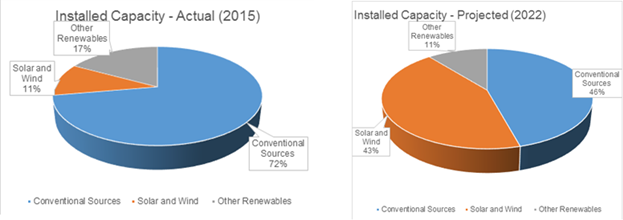
\includegraphics[scale=1]{Intro1}
\caption{Actual and Projected Installed Electricity Generation Capacity Distribution}
\label{figc1h1} %% to refer use, \ref{}
\end{figure}

The Indian electricity grid is working in an archaic mode, where it’s operational practices and control mechanisms are tuned to serve a grid dominated by Thermal Power Stations (Fossil Fueled and Nuclear) which provide for base load and Hydro Power Stations providing for peak load. The energy output of these two kinds of power plants is deterministic and hence are easier to schedule.\\

But, the energy output of Solar and Wind Power Plants depends on the weather conditions and is stochastic and not deterministic and on most occasions delivers power lower than its installed capacity, which is a real problem for grid operators. Only an accurate forecast of power can solve the problem of efficient renewable energy scheduling (Electricity sector in India, n.d.).\\

At the moment there have only been two pilot projects for wind energy forecasting; one in Gujarat that completed in February 2015 with 30\% inaccuracy of forecasts; not due to the inefficiency of the participating companies (all were foreign private companies) but due to the lack of data; the other one has started in Tamil Nadu by a company called Vortex in cooperation with NIWE (National Institute of Wind Energy). There is no forecasting pilot project for solar yet ( Richts, Strauß, & Heinemann, 2015).\\

Hence development of an indigenous renewable energy/power forecasting application for solar photovoltaic and wind power plants is of paramount importance. So that, by 2022 when almost 43\% of the installed generation capacity will consist of SPV and Wind power plants, we will have a robust renewable generation forecasting application to take care of the intermittent nature of energy generation.




\section{Literature Review}
\
\
\
\
Owing to the stochastic nature of the weather variables (Irradiance, Temperature and Wind Speed), the energy/power generation output from Solar Photovoltaic (SPVPP) and Wind Turbine Power Plants (WTPP) is also stochastic i.e. undeterministic. The control and operation of conventional electricity grids depend on the assumption that generation is deterministic and the load is undeterministic. Hence, it becomes a great challenge to perform optimal scheduling, unit commitment and load-balancing in grids where there is a large penetration of SPVPs and WTPPs without accurate generation forecasts.
It is self-evident that that undeterministic generation from SPVPs and WTPPs is the direct result of the stochastic nature of the weather variables which drive these systems. Therefore, for accurate generation forecasting of these systems, we need to forecast the driving weather variables accurately. These forecasted weather variables can then be fed as inputs to the deterministic energy/power estimation models for SPVP and WTPP as described in (Masters, 2004) and (Patel, 2006) respectively. Hence, the forecasting should done for driving weather variables, and the energy/power forecasts for SPVPs and WTPPs should be done indirectly by using the energy/power estimation models. 
A holistic study of the current techniques used for weather variable forecasting shows us that Autoregressive Integrated Moving Average models (ARIMA), Artificial Neural Networks (ANN) and Numerical Weather Prediction systems (NWP) are at the forefront of the forecasting technology horizon. ARIMA and ANN are accurate for intra-hour and intra-day irradiance forecasting; whereas NWPs like ECMWF (European Centre for Mesoscale Weather Forecasting) and WRF (Weather Research and Forecasting) are accurate for day-ahead irradiance forecasting ( Diagna, David, Lauret, Boland, & Schmutz, 2013). ANN with back propagation can be used successfully for wind speed forecasts, and similar ANN models can be used for forecasting other weather variables like Dew-Point Temperature, Relative Humidity, Wind Direction and Pressure (Upadhyay, Choudhary, & Tripathi, 2011). ANN and ARIMA are good for short-term wind speed forecasting, whereas NWP models predict wind speed better than statistical models; moreover, hybrid models employing combination of the before mentioned techniques are the most accurate for wind speed prediction ARIMA (Saroha & Aggarwal, 2015).  ANN and NWP are the best model choices for wind speed prediction ( Zhu & Genton, 2012). Hence, we can conclude that ARIMA, ANN and NWP methods are a good choice for short-term (intra-hour and intra-day; ANN and ARIMA) and long-term (day-ahead; NWP) weather variable forecasting; in addition, hybrid forecasting models based on these techniques can improve the accuracy of the forecast (Chang, 2014).\\

The classical method of time series modelling propagated by the statisticians Box and Jenkins in the 70’s, and still used today. Their models of ARMA (Autoregressive Moving Averages, for stationary time series) and ARIMA (Autoregressive Integrated Moving Averages, for non-stationary time series) provide building blocks for creating the most basic statistical forecasts based on the time series’ mean and variance values. ARIMA models for weather forecasting are developed by examining Auto-Correlation Function (ACF) and Partial Auto-Correlation Function (PACF), the best models are selected based on the lowest values of Akalike Information Criterion (AIC) and Bayesian Information Criterion (BIC) ( Shamsnia, Shahidi, Liaghat, Sarraf, & Vahdat, 2011). Hybrid models consisting of Multi-Linear Regression (MLR) and ARIMA outperform usual ARIMA and ANN models for weather prediction (Sharma, 2012). ARIMA and Artificial Neuro Fuzzy Inference System (ANFIS) are compared for weather forecasting, it is observed that AFIS performs better than ARIMA, as it is a hybrid system (Tektas, 2010). ARIMA and ANN both are good for time series weather forecasting, however hybrid ARIMA-ANN outperforms both techniques by reducing model uncertainty (Zhang, 2003). For short-term irradiance forecasting ARIMA models outperform NWP, and predict accurately in the time frame of 5 minutes to 4 hours, but NWP perform superiorly better for day-ahead irradiance forecasting ( Prajapati & Sahay, 2016) and ( Kaushik & Singh, 2008).ARIMA models have been developed using Box-Jenkins methodology for predicting accurately monthly values for temperature, rainfall and relative humidity in Ahvaz, Iran and districts of Sri Lanka (Sarraf, Vahdat, & Behbahaninia, 2011), (Partheepan & Jeyakumar, 2005) and (Nurry, Koch, & Alam). Non-Linear Autoregressive Exogenous Artificial Neural Network (NARX) performs better than ARIMA being a non-linear model for wind speed time series one-step ahead prediction (Cadenas, Rivera, Campos-Amezcua, & Heard, 2016). Hence, ARIMA models have been applied successfully for short-term forecasting of irradiance, temperature and wind speed, using the ACF and PACF examination approach in combination with AIC and BIC for selecting the best model; moreover, hybrid models of ARIMA with other techniques are superior but complex as compared to usual ARIMA models for weather variable prediction.\\

The modern technique of Artificial Neural Networks, which are inspired from biological neural networks. They work on the principle of interconnected neurons forming a network between inputs and outputs; the neurons consists of a mathematical function, biases and weights. This network of neurons is made to learn the data during training phase using appropriate learning methods. ANN’s can be trained to do a variety of jobs; namely Clustering, Classification and Regression. For weather variable forecasting we need to develop a neural network for solving a regression problem. ANN trained with back propagation (BP) algorithm can approximate large class of non-linear functions; hence, it can be used in weather prediction, the only requirement for good predictions being good quality historical data (Reddy, Devi, Kumar, Reddy, & Nayak, 2012).  Multi-Layer Perceptron model (MLP) has the potential to be successfully applied to weather forecasting (Kumar & Jha, 2013). MLP with BP is an ideal solution for predicting dynamic and non-linear weather processes, it is better than traditional numerical methods (Malik, Singh, & Arora, 2014). Various weather variables like rainfall, wind speed, irradiance and temperature can be forecasted accurately using MLP and Radial Basis Function Network (RBFN) (Shrivastava, Karmakar, Korwar, & Guhathakurta, 2012). . When MLP RBFN, Elman Recurrent Neural Network (ERNN) and Hopfield Model (HFM) are compared, MLP and RBFN perform weather accurate weather forecasts comparatively (Maqsood, Khan, & Abraham, 2004). A hybrid model using ARIMA which is a linear model and ANN which is a non-linear model, irradiance can be predicted accurately for both clear and cloudy days ( Voyant, Muselli, Paoli, & Nivet). To improve irradiance forecasts further additional inputs of irradiance derivatives can be used, which improves irradiance forecast under changeable weather conditions (Wang, et al., 2016). For a shot-term irradiance forecast ANN outperforms NWP (Cornaro, et al.). Also, temperature prediction with greater accuracy can be done by training one ANN model for each season (Hayati & Mohebi, Temperayure Forecasting Based on Neural Network Approach, 2007). Ensemble ANN model for temperature forecasting improves accuracy to a great extent (Kadu, Wagh, & Chatur). ANN outperforms ARIMA model for short-term wind speed forecasting (Catalao, Pousinho, & Mendes, 2009). Hence, incorporating ensemble and hybrid modeling strategy with ANN can help predict irradiance, temperature and wind speed to a high accuracy for a short-term forecast.\\

The Numerical Weather Prediction Models (NWP’s) like ECMWF and WRF they produce good weather forecasts up to 1km spatial and about 3min temporal resolution. NWP’s are quite different from the first two forecasting techniques as they depend on accurate physical descriptions of the atmospheric processes and tend to give highly accurate forecasts. But, the problem here is these softwares require supercomputers to run them as they require a lot of computing power and memory. The WRF is a next generation NWP with efficiency, portability, maintainability and extensibility at its core architecture; being open source and community driven, it has fostered communication, cooperation, collaboration within WRF working groups specializing in regional climate, air quality simulation, and NWP research (MICHALAKES,, et al., 2005). WRF model was used for forecasting energy production of a SPVP, WRF weather variables and the historical plant power production data was used to train a Quantile Regression Forest forecast model; it is observed that accuracy of daily energy forecasts is greater than hourly predictions (Almeidaa, Lamigueirob, & Narvarte). Improved power forecast for SPVP and WTPP is carried out using a hybrid model of linear regression of forecasted outputs of the WRF model, this model outperforms the usual WRF model ( Avolio, et al., 2016).  The GHI prediction from WRF are not accurate, but are usually over-estimated due to WRF’s inability to model clouds, aerosols, ozone properly also the radiation models used in WRF are good drivers for atmospheric processes but not so much for precise surface solar irradiances; hence post processing of GHI is required for accurate prediction, some methods are: Spatial Averaging, Incorporating Ozone and Aerosols using satellite retrievals, Kalman Filters, and Recursive method and Assimilating cloud cover data into the WRF initialization using GOES satellite imagery; as mentioned in (Larson, Nonnenmacher, & Coimbra, 2016), ( Lara-Fanego, Ruiz-Arias, Pozo-Va´zquez, Santos-Alamillos, & Tovar-Pescador, 2011), (Rincón, Jorba, Baldasano, & Monache, 2011), (Mathiesen, et al., 2014) and (Heinemann, Lorenz, & Girodo) respectively. Another method to improve the GHI forecasts from the WRF, an ensemble WRF model is suggested where linear combination of one or more WRF runs for the same location with different initial and boundary conditions is done, this improves the GHI forecast by reducing the uncertainty associated to the initial and boundary meteorological conditions (Díaz, Souto, Rodríguez, Saavedra, & Casares, 2012). The land surface schemes responsible for computing heat and moisture fluxes over the land surface overestimate, for improving the temperature and wind speed forecast from WRF model a good post-processing system has to be used ( Khvorostyanov, Menut, Dupont, Morille,, & Haeffelin). The YSU scheme in WRF with an ensemble mean with a GFS (Global Forecast System) initialized WRF model is the best for wind speed prediction ( Rabideau). The ARW user manual provides excellent documentation of the installation and running of the WRF software (Wang, et al., 2016). The comparison of the two dynamic solvers within WRF which are the Advanced Research WRF (ARW) and the Non-hydrostatic Mesoscale Model (NMM), shows that there is no difference in the WRF output with the change in the dynamic solvers ( Bernardet, et al.). Hence, WRF is proved to be a great tool for mesoscale weather prediction and it has been used successfully for day-ahead weather forecasting in relation to SPVP and WTPP generation forecasting; moreover, with good parameterization of the WRF model options, appropriate post-processing systems and ensemble models the WRF system can be used for very accurate day-ahead forecast of the SPVP and WTPP generation.\\

To summarize, the problem of solar and wind energy/power forecasting can be broken down into two parts: the energy estimation part and the weather variable forecasting part. The weather variable forecasting can be done using ANN and ARIMA for short-term i.e. intra-hour and intra-day periods; whereas NWP like WRF can be used for day-ahead forecasting of weather variables. These forecasted weather variables can then be used as input to the energy estimation models which will compute the forecasted energy/power for the SPVP and WTPP. A HADOOP based ARIMA weather forecasting has been developed using HBASE and SQOOP for database management, this shows that for forecasting systems to be scalable and usable they have to be developed as an application so that routines are automised (Li, Ma, Liu, & Fan, 2013). Figure 3 shows the schematic of the forecasting procedure, but in order to achieve this an indigenous application has to be designed and developed; which will make it easy to train and develop ANN and ARIMA models as well as automate the process of running a WRF, and energy estimation of SPVP and WTPP. This thesis intends to develop a complete application which can function as a platform for solar and wind energy estimation and forecasting.


\section{Contribution to Scientific Community}
\
\
\
\
The process of generation forecasting of SPVP and WTPP includes: Data acquisition, Data pre-processing, Selection of appropriate mathematical forecasting model (i.e. ARIMA, ANN or WRF), Forecast model development, Forecast model testing and finally the Forecast model implementation. All these steps require different softwares and/or Application Programming Interfaces (API's) to work as a cohesive unit to get forecasting done. The work done in this thesis tries to bring together all the aforementioned steps under one umbrella, to make the forecaster's job a little lucid. The Fig (\ref{figc1h2}) shows the block diagram of forecasting model developed, here the stochastic weather variables are forecasted using the different mathematical models, and these forecasted weather variables are fed as inputs to the deterministic energy estimation models for SVPP and/or WTPP to get the energy/power forecasts as desired.
`	`																		`  

\begin{figure}[H]
\centering
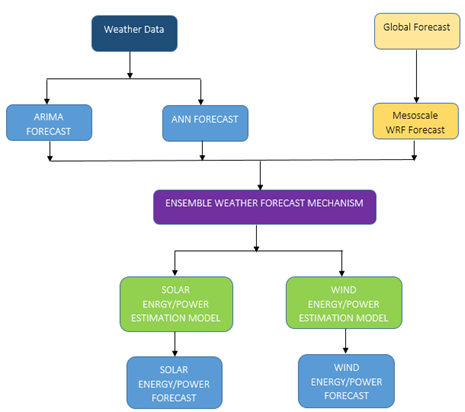
\includegraphics[scale=1]{Intro2}
\caption{Block Diagram – Ensemble Solar/Wind Power Forecasting}
\label{figc1h2} %% to refer use, \ref{}
\end{figure}

The Fig (\ref{figc1h3}) illustrates the application structure developed in MATLAB using its GUI feature. The application performs all the steps mentioned earlier to get the generation forecast through an easy to use GUI interface. Moreover, the application has been coded with modularity at the heart of its design; which makes it easy to upgrade, change and debug as desired by the forecaster. 

\begin{figure}[H]
\centering
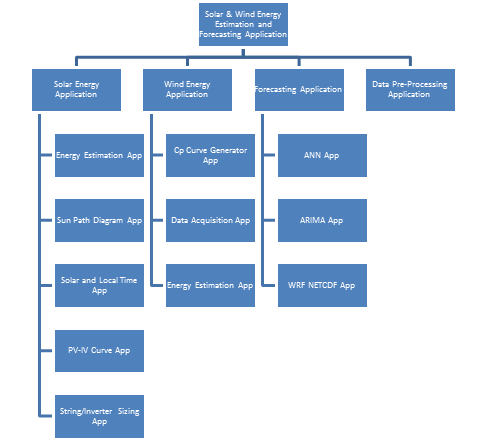
\includegraphics[scale=1]{Intro3}
\caption{Organization Structure of Application}
\label{figc1h3} %% to refer use, \ref{}
\end{figure}

The application can act as a complete software package for energy estimation and generation forecasting for SVPP and WTPP, and be a solid foundation for developing a real-time generation forecasting system.\\

\chapter{Data of Gujarat Solar PV Plants}
%% Chapter 2 : Data of Gujarat Solar PV Plants

\section{Intro}
\
\
\
\
Historical solar generation data is the most important resource along with historical weather data to model highly accurate prediction systems for Solar PV generation. The data used in this thesis is obtained from the Gujarat State Load Dispatch Centre (SLDC). Some analysis has been done on the raw data from SLDC to convert it into valuable information which can be used to great effect in the thesis.

\section{Solar Generation in Gujarat}
\
\
\
\
The following table lists the Solar PV plants operational in Gujarat as of August, 2015. The Table \ref{tabc2h1} gives information about the name of the plant,  the latitudes and longitudes and commissioned capacity. The generation data from 2012 to August of 2015 has been procured from the SLDC
\\

\begin{table}[H]
  \centering
%%From Excet to LATEX Add-In  
   \caption{List of Solar PV Plants in Gujarat}

    \begin{tabular}{|l|c|c|c|}
    \hline
    \textbf{Company Name} & \textbf{Lat } & \textbf{Long } & \textbf{Commissioned, MW} \bigstrut\\
    \hline
    Sunkon Energy Pvt. Ltd. & \textbf{20.9} & \textbf{71.3} & \textbf{10} \bigstrut\\
    \hline
    ACME Solar Technologies (Gujarat) Pvt. Ltd. & \textbf{22.3} & \textbf{72.4} & 15 \bigstrut\\
    \hline
    Precious Energy Services Pvt. Ltd. & \textbf{23.9} & \textbf{71.9} & \textbf{15.2} \bigstrut\\
    \hline
    Sandland Real Estate Pvt. Ltd. & \textbf{24.5} & \textbf{72.2} & \textbf{25} \bigstrut\\
    \hline
    Solitaire Energies Pvt. Ltd. & \textbf{23.9} & \textbf{71.9} & \textbf{15.01} \bigstrut\\
    \hline
    TATA Power Renewable Energy Ltd. & \textbf{22.4} & \textbf{69.0} & \textbf{25} \bigstrut\\
    \hline
    Mono Steel (India) Ltd. & \textbf{22.8} & \textbf{71.0} & \textbf{10} \bigstrut\\
    \hline
    Adani Enterprises Ltd. & \textbf{23.3} & \textbf{69.0} & 40.11 \bigstrut\\
    \hline
    Backbone Enterprises Ltd. & \textbf{23.4} & \textbf{70.6} & 5 \bigstrut\\
    \hline
    Euro Solar Power Pvt Ltd & \textbf{23.4} & \textbf{70.6} & \textbf{5.12} \bigstrut\\
    \hline
    Gujarat Mineral Development Company Ltd. & \textbf{23.8} & \textbf{68.8} & \textbf{5} \bigstrut\\
    \hline
    Integrated Coal Mining Ltd. & \textbf{23.4} & \textbf{70.7} & \textbf{9} \bigstrut\\
    \hline
    Konark Gujarat PV Pvt. Ltd. & \textbf{23.4} & \textbf{70.6} & \textbf{5} \bigstrut\\
    \hline
    Solar Semiconductor Power Company ( India) Pvt Ltd & \textbf{23.4} & \textbf{70.6} & \textbf{20} \bigstrut\\
    \hline
    Sunborne Energy Gujarat One Pvt.Ltd. & \textbf{23.4} & \textbf{70.4} & \textbf{15} \bigstrut\\
    \hline
    Unity Power Private Ltd.  & \textbf{23.4} & \textbf{70.1} & \textbf{5} \bigstrut\\
    \hline
    Welspun Urja Gujarat Pvt. Ltd. & \textbf{23.4} & \textbf{70.1} & \textbf{15.01} \bigstrut\\
    \hline
    AES Solar Energy Gujarat Pvt. Ltd. & \textbf{23.9} & \textbf{71.2} & 14.92 \bigstrut\\
    \hline
    Alex Astral Power Pvt. ltd. & \textbf{23.9} & \textbf{71.2} & 25.07 \bigstrut\\
    \hline
    Astonfield Solar (Gujarat) Private Limited  & \textbf{23.7} & \textbf{71.7} & 11.51 \bigstrut\\
    \hline
    Avtar Solar Power Pvt Ltd & \textbf{23.9} & \textbf{71.2} & 4.98 \bigstrut\\
    \hline
    Emami Cement Ltd. & \textbf{23.9} & \textbf{71.2} & \textbf{10.06} \bigstrut\\
    \hline
    GMR Gujarat Solar Power Pvt. Ltd. & \textbf{23.9} & \textbf{71.2} & \textbf{25} \bigstrut\\
    \hline
    GSPC Pipavav Power Company Limited & \textbf{23.9} & \textbf{71.2} & \textbf{5} \bigstrut\\
    \hline
    Jaihind Projects Ltd. & \textbf{23.9} & \textbf{71.2} & \textbf{5} \bigstrut\\
    \hline
    Kindle Engg \& Const Pvt Ltd & \textbf{23.9} & \textbf{71.2} & \textbf{50} \bigstrut\\
    \hline
    Lanco Infratech Ltd & \textbf{23.9} & \textbf{71.2} & \textbf{15.01} \bigstrut\\
    \hline
    Lanco Infratech Ltd (BHRD) & \textbf{23.7} & \textbf{71.6} & \textbf{5} \bigstrut\\
    \hline
    Lanco Infratech Ltd (Chandiyana) & \textbf{23.7} & \textbf{71.6} & \textbf{15.01} \bigstrut\\
    \hline
    NKG Infrastructure Ltd. & \textbf{23.9} & \textbf{71.2} & \textbf{10} \bigstrut\\
    \hline
    \end{tabular}%

%% All above Code is copied from Excel to LATEX Add-In 
    %\caption{Add caption}
    \label{tabc2h1}%

\end{table}

\begin{table}[H]
  \centering
%%From Excet to LATEX Add-In  
    \begin{tabular}{|l|c|c|c|}
    \hline
    \textbf{Company Name} & \textbf{Lat (N)} & \textbf{Long (E)} & \textbf{Commissioned, MW} \bigstrut\\
    \hline
    Palace Solar Energy Pvt. Ltd. & \textbf{23.9} & \textbf{71.2} & \textbf{15} \bigstrut\\
    \hline
    PLG Photovoltaics Ltd & \textbf{23.9} & \textbf{71.5} & \textbf{20} \bigstrut\\
    \hline
    Roha Dyechem Pvt. Ltd. & \textbf{23.9} & \textbf{71.2} & \textbf{25.04} \bigstrut\\
    \hline
    Solarfield Energy Private Limited & \textbf{23.8} & \textbf{71.2} & \textbf{20.06} \bigstrut\\
    \hline
    Sun Clean Renewable Power Pvt. Ltd. & \textbf{23.9} & \textbf{71.2} & \textbf{6} \bigstrut\\
    \hline
    Surana Telecom \& Power Ltd. & \textbf{23.9} & \textbf{71.2} & \textbf{5} \bigstrut\\
    \hline
    Torrent Solargen Limited & \textbf{23.9} & \textbf{71.2} & \textbf{51} \bigstrut\\
    \hline
    Yantra eSolar India Pvt. Ltd. & \textbf{23.9} & \textbf{71.2} & \textbf{4.95} \bigstrut\\
    \hline
    Gujarat Power Corporation Ltd. & \textbf{23.9} & \textbf{71.2} & \textbf{5} \bigstrut\\
    \hline
    SEI Solar Power Gujarat Pvt. Ltd. & \textbf{23.9} & \textbf{71.2} & \textbf{25.01} \bigstrut\\
    \hline
    ZF Steering Gear(India) Pvt. Ltd. & \textbf{23.9} & \textbf{71.2} & \textbf{5} \bigstrut\\
    \hline
    GHI Energy Pvt. Ltd. (SPV of Refex) & \textbf{21.6} & \textbf{69.9} & \textbf{10} \bigstrut\\
    \hline
    Hiraco Renewable Energy Pvt. Ltd. & \textbf{21.6} & \textbf{69.9} & \textbf{20.11} \bigstrut\\
    \hline
    Moserbaer Energy \& Development Ltd. & \textbf{21.6} & \textbf{69.9} & \textbf{15.02} \bigstrut\\
    \hline
    APCA Power Pvt. Ltd. & \textbf{21.8} & \textbf{70.1} & 5 \bigstrut\\
    \hline
    Aravali Infrapower Ltd. & \textbf{21.8} & \textbf{70.1} & 5 \bigstrut\\
    \hline
    CBC Solar Technologies Pvt. Ltd.  & \textbf{21.7} & \textbf{70.1} & 10 \bigstrut\\
    \hline
    Ganeshvani Merchandise Pvt Ltd & \textbf{21.7} & \textbf{70.1} & \textbf{5.04} \bigstrut\\
    \hline
    Ganges Green Energy Pvt Ltd. & \textbf{21.7} & \textbf{70.1} & \textbf{25.08} \bigstrut\\
    \hline
    Green Infra Solar Energy Ltd. & \textbf{21.7} & \textbf{70.1} & \textbf{10} \bigstrut\\
    \hline
    Taxus Infrastructure \& Power Project Pvt.Ltd & \textbf{23.3} & \textbf{70.0} & \textbf{5} \bigstrut\\
    \hline
    Aatash Power Pvt. Ltd. & \textbf{23.6} & \textbf{73.3} & 4.99 \bigstrut\\
    \hline
    Azure Power (Haryana) Pvt. Ltd. & \textbf{23.4} & \textbf{73.2} & 10.21 \bigstrut\\
    \hline
    Gujarat Industries Power Company Ltd. & \textbf{21.4} & \textbf{73.1} & \textbf{5.01} \bigstrut\\
    \hline
    Azure Power (Gujarat) Pvt. Ltd. & \textbf{23.2} & \textbf{71.4} & 5 \bigstrut\\
    \hline
    Chattel Constructions Private Ltd. & \textbf{23.3} & \textbf{71.8} & 25.04 \bigstrut\\
    \hline
    Dreisatz MySolar24 (P) Ltd. & \textbf{23.4} & \textbf{71.6} & 14.99 \bigstrut\\
    \hline
    EMCO Ltd. & \textbf{23.4} & \textbf{71.6} & \textbf{5} \bigstrut\\
    \hline
    ESP Urja Pvt. Ltd. & \textbf{23.5} & \textbf{71.7} & \textbf{5} \bigstrut\\
    \hline
    Louroux Bio Energies Ltd.  & \textbf{22.7} & \textbf{71.4} & \textbf{25} \bigstrut\\
    \hline
    \end{tabular}%

%% All above Code is copied from Excel to LATEX Add-In 
    %\caption{Add caption}
    %\label{}%

\end{table}

\begin{table}[H]
  \centering
%%From Excet to LATEX Add-In  
    \begin{tabular}{|l|c|c|c|}
    \hline
    \textbf{Company Name} & \textbf{Lat (N)} & \textbf{Long (E)} & \textbf{Commissioned, MW} \bigstrut\\
    \hline
    MI MySolar24 (P) Ltd,  & \textbf{23.4} & \textbf{71.6} & \textbf{14.99} \bigstrut\\
    \hline
    Millennium Synergy (Gujarat) Pvt. Ltd. & \textbf{23.4} & \textbf{71.7} & \textbf{9.27} \bigstrut\\
    \hline
    Responsive sutip ltd. & \textbf{23.1} & \textbf{71.9} & \textbf{25.06} \bigstrut\\
    \hline
    S J Green Park Energy Pvt. Ltd & \textbf{22.7} & \textbf{71.4} & \textbf{5.12} \bigstrut\\
    \hline
    Ujjawala Power Pvt Ltd & \textbf{23.1} & \textbf{71.9} & \textbf{23.06} \bigstrut\\
    \hline
    Visual Percept Solar Projects Pvt. Ltd. & \textbf{23.5} & \textbf{71.6} & \textbf{25} \bigstrut\\
    \hline
    Waa Solar Pvt. Ltd. & \textbf{22.7} & \textbf{71.4} & \textbf{10.25} \bigstrut\\
    \hline
    SSNL, SAMA & \textbf{22.3} & \textbf{73.2} & \textbf{10} \bigstrut\\
    \hline
       & \textbf{} & \textbf{Total} & \textbf{852.31} \bigstrut\\
    \hline
    \end{tabular}%


%% All above Code is copied from Excel to LATEX Add-In 
    %\caption{Add caption}
    %\label{}%

\end{table}
\\
All the above mentioned Solar Plants were located and tagged on a Google Earth File for ease of access to their geometric design for creating accurate shading analysis in PVsyst Software. The Fig \ref{figc2h1} shows a snapshot of the Google Earth File.
\\
\begin{figure}[H]
\centering
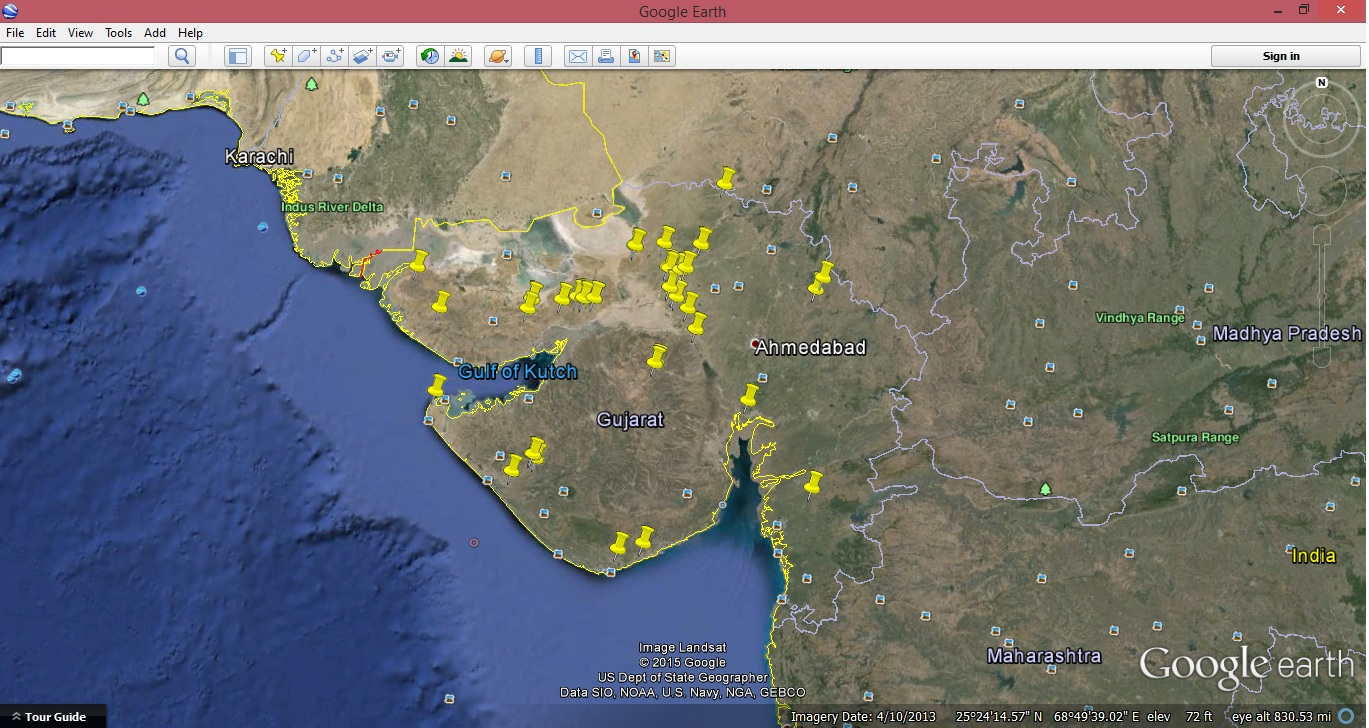
\includegraphics[scale=0.5]{GoogleEarthGuj}
\caption{Google Earth View of Solar PV Plants \geq 5MW in Gujarat}
\label{figc2h1} %% to refer use, \ref{}
\end{figure}
\\
The Fig \ref{figc2h2} gives the monthly solar energy generated by the PV plants given in Table \ref{tabc2h1} for four years from 2012 till August, 2015.
\\
\begin{figure}[H]
\centering
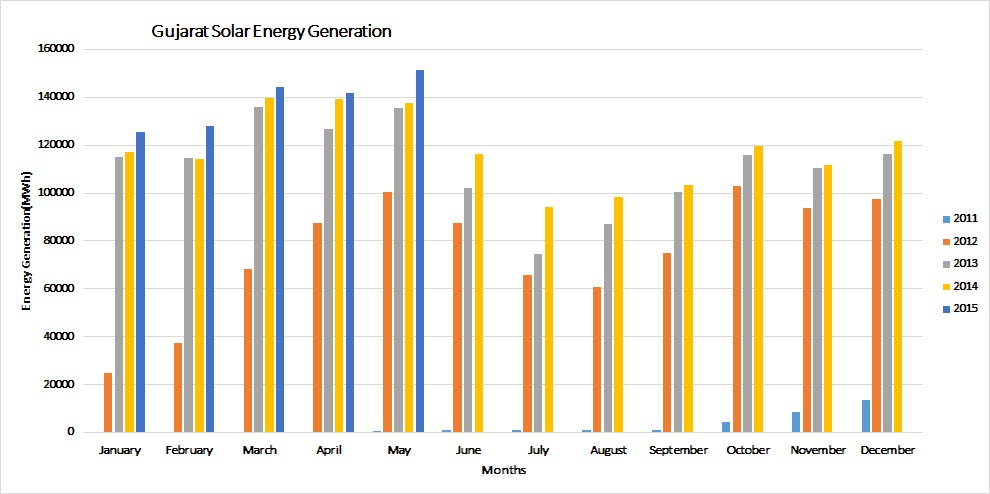
\includegraphics[scale=0.65]{Guj1}
\caption{Monthly Solar Power Generation in Gujarat as of Aug 2015}
\label{figc2h2} %% to refer use, \ref{}
\end{figure}
\\
The Capacity Utilization Factor (CUF)is very good measure of the efficiency of any power plant. The CUF of the entire generating capacity of PV plants in Table  \ref{tabc2h1} is calculated and presented in Fig.\ref{figc2h3}, which shows a rising efficiency of PV Power Plants in Gujarat over the course of 4 years.
\\

\begin{figure}[H]
\centering
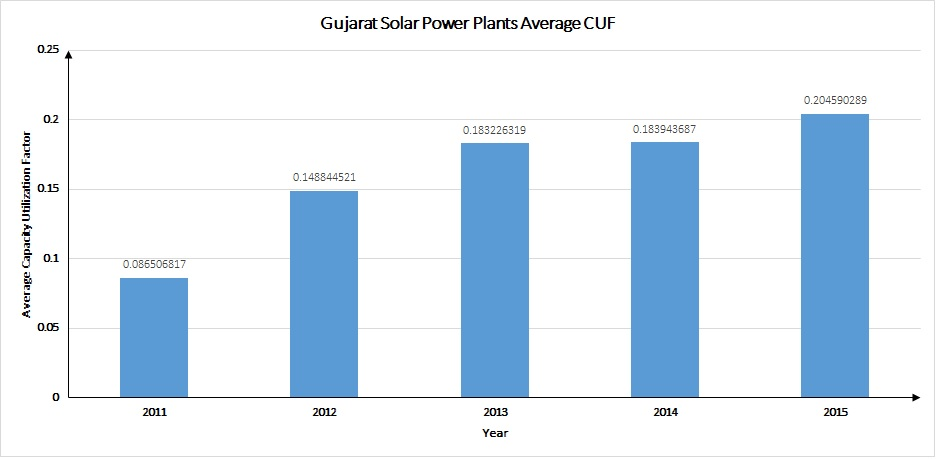
\includegraphics[scale=0.65]{Guj2}
\caption{Capacity Utilization Factor (CUF) for entire Gujarat}
\label{figc2h3} %% to refer use, \ref{}
\end{figure}

\newpage

\section{District-Wise Solar Energy Generation in Gujarat}
\
\
\
\
The data belonging to the Solar Plants in Fig \ref{tabc2h1} is segregated district-wise, it gives some really good insights. The Table \ref{tabc2h2} contains the capacity, average yearly energy generation, average yearly CUF and average yearly MWh/MW data.
\\ 
\begin{table}[H]
  \centering
%%From Excet to LATEX Add-In  
\caption{Gujarat District-Wise Solar Energy Data}
    \begin{tabular}{|r|c|c|r|r|}
    \hline
       & \textbf{Allotted,MW} & \textbf{CUF} & \multicolumn{1}{c|}{\textbf{Energy/Year}} & \multicolumn{1}{c|}{\textbf{MWh/MW}} \bigstrut\\
    \hline
    \textbf{Amreli} & 10 & 0.174114 & 9360.5402 & 936.054 \bigstrut\\
    \hline
    \textbf{Anand} & 15 & 0.147882 & 15591.016 & 1039.401 \bigstrut\\
    \hline
    \textbf{Banaskantha} & 55 & 0.18076 & 61724.444 & 1122.263 \bigstrut\\
    \hline
    \textbf{Jamnagar} & 25 & 0.162181 & 29841.603 & 1193.664 \bigstrut\\
    \hline
    \textbf{Junagadh} & 10 & 0.173891 & 11885.173 & 1188.517 \bigstrut\\
    \hline
    \textbf{Kutch} & 129 & 0.160941 & 132019.11 & 1023.404 \bigstrut\\
    \hline
    \textbf{Patan} & 397.5 & 0.166076 & 308645.3 & 776.4662 \bigstrut\\
    \hline
    \textbf{Porbandar} & 45 & 0.150004 & 49970.088 & 1110.446 \bigstrut\\
    \hline
    \textbf{Rajkot} & 60 & 0.165073 & 57596.477 & 959.9413 \bigstrut\\
    \hline
    \textbf{Sabarkantha} & 15 & 0.162073 & 17215.268 & 1147.685 \bigstrut\\
    \hline
    \textbf{Surat} & 5  & 0.14309 & 5229.0196 & 1045.804 \bigstrut\\
    \hline
    \textbf{Surendranagar} & 195 & 0.14968 & 177200.73 & 908.7217 \bigstrut\\
    \hline
    \textbf{Vadodara} & 10 & 0.064522 & 1009.5442 & 100.9544 \bigstrut\\
    \hline
    \end{tabular}%

%% All above Code is copied from Excel to LATEX Add-In 
    %\caption{Add caption}
    \label{tabc2h2}%

\end{table}
\\
The Fig \ref{figc2h4} shows the district-wise solar energy generation in gujarat. We can see that Patan leads all the districts in energy production (due to largest number of solar plants ) whereas Vadodara has the lowest energy production.
\\

\begin{figure}[H]
\centering
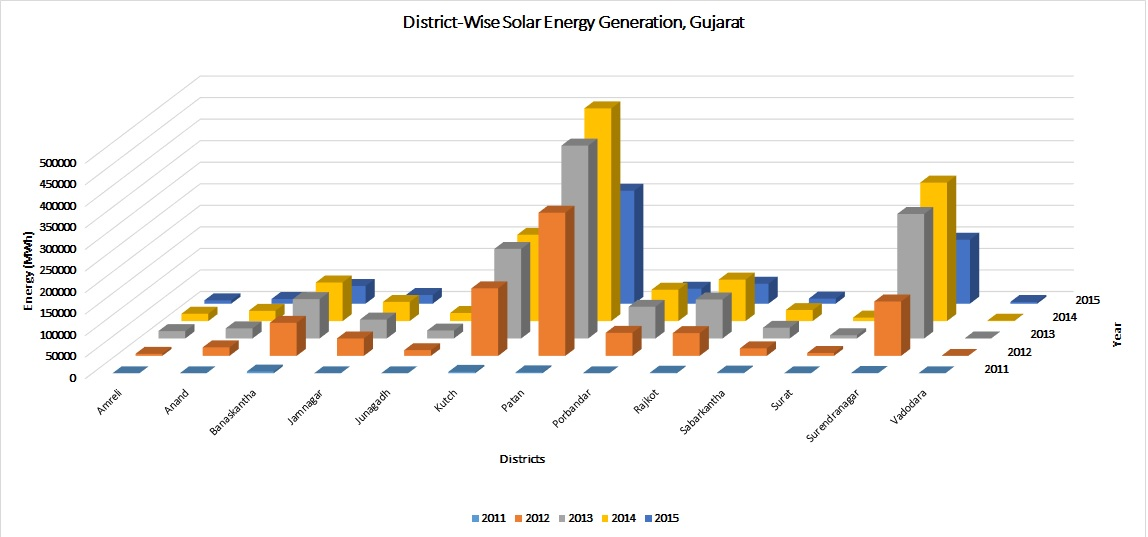
\includegraphics[scale=0.65]{Dist2}
\caption{District-Wise Solar Energy Generation in Gujarat}
\label{figc2h4} %% to refer use, \ref{}
\end{figure}
\\
The Fig \ref{figc2h5} shows the district-wise MWh/MW, it is also a good indicator of the efficiency of the solar power produced. We can see that over the years these values for each state have increased and Junagadh shows the highest MWh/MW value, while Patan shows the lowest MWh/MW value.
\\

\begin{figure}[H]
\centering
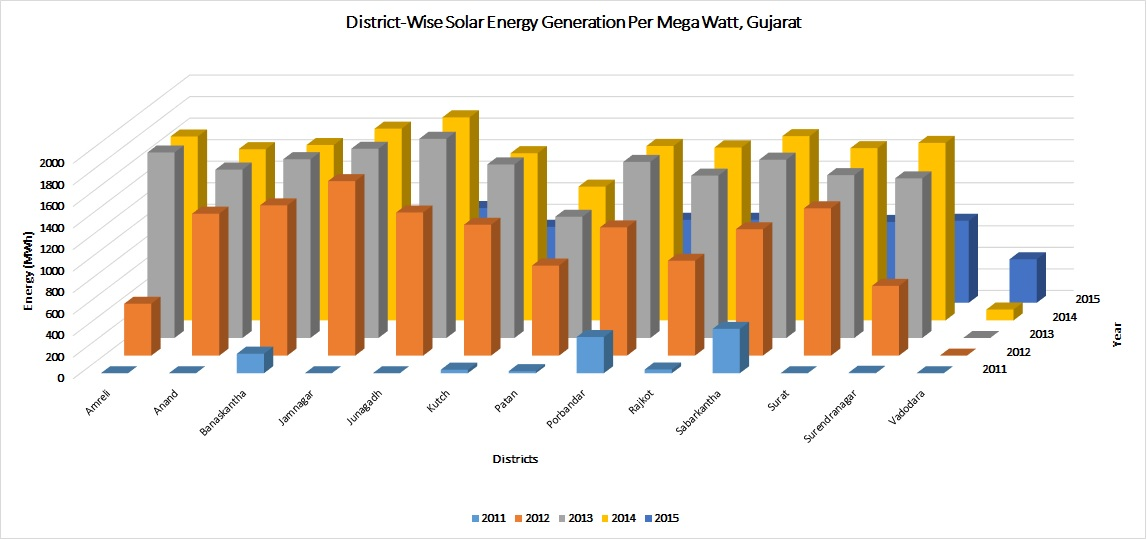
\includegraphics[scale=0.65]{Dist3}
\caption{District-Wise MWh/MW in Gujarat}
\label{figc2h5} %% to refer use, \ref{}
\end{figure}
\\
The Fig \ref{figc2h6} shows the district-wise CUF in Gujarat. We can see that similar to the last graph here to Junagadh has the highest value and Patan has the lowest value. We can say that CUF and MWh/MW have a good correlation, and they show efficiency of energy generation in different ways but of similar forms.
\\

\begin{figure}[H]
\centering
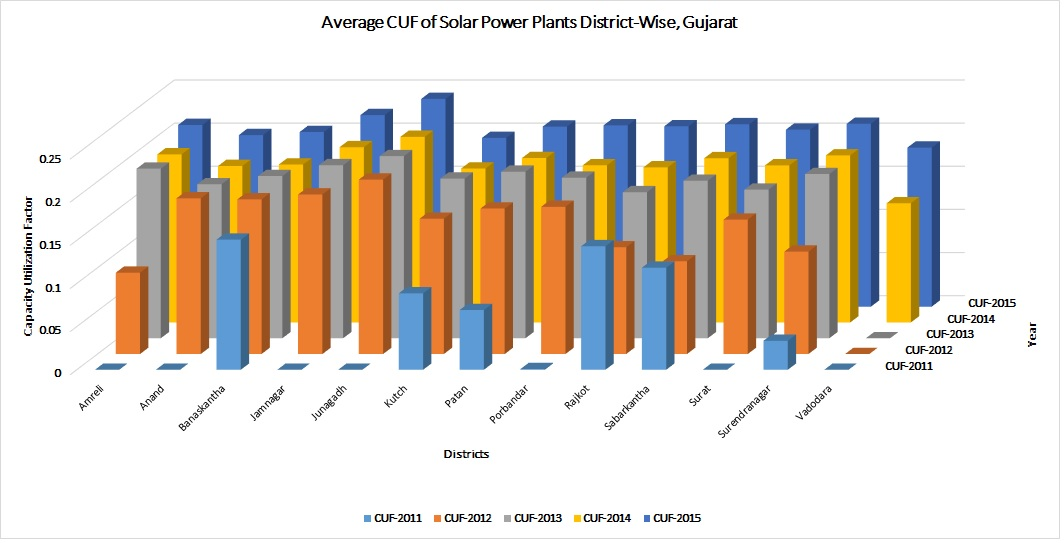
\includegraphics[scale=0.65]{Dist1}
\caption{District-Wise Capacity Utilization Factor (CUF) in Gujarat}
\label{figc2h6} %% to refer use, \ref{}
\end{figure}

\section{Charanka Solar Park Analysis on the basis of PV Technology}
\
\
\
\
Charanka Solar Park in Patan district is Gujarat's largest Solar park as of August, 2015 with eighteen solar power plants and a total capacity of 272MW. Models of all the eighteen solar plants were simulated in PVsyst software and an analysis of performance of Mono-Crystalline (Mono), Poly-Crystalline (Poly) and Thin Film (Thin) PV technologies has been carried out. The Table \ref{tabc2h3} gives the results of that analysis values which have a letter P after them are simulated quantities and others are real quantities.
\\
\begin{table}[H]
  \centering
  \caption{Charaka Solar Park Analysis}
%%From Excet to LATEX Add-In  
    \begin{tabular}{|c|l|l|l|l|l|l|}
    \hline
    \textbf{} & \textbf{Name} & \textbf{MW} & \textbf{MWh} & {\textbf{MWh P}} & \textbf{MWh/MW} & \textbf{MWh/MW P} \bigstrut\\
    \hline
    \textbf{Mono} & LANCO  & 15.0 & 20506.3 & 27379.0 & 1367.1 & 1825.3 \bigstrut\\
\cline{2-7}       & \textbf{Tot Energy} & \textbf{15.0} & \textbf{20506.3} & \textbf{27379.0} &    &  \bigstrut\\
\cline{2-7}       & \textbf{MWh/MW} &    & \textbf{1367.1} & \textbf{1825.3} &    &  \bigstrut\\
\cline{2-7}       & \textbf{Average} &    &    &    & \textbf{1367.1} & \textbf{1825.3} \bigstrut\\
    \hline
    \textbf{Poly } & GSPC  & 5.0 & 8906.5 & 8358.0 & 1781.3 & 1671.6 \bigstrut\\
\cline{2-7}       & Surana  & 5.0 & 7899.3 & 9053.0 & 1579.9 & 1810.6 \bigstrut\\
\cline{2-7}       & NKG  & 10.0 & 17729.4 & 17168.0 & 1772.9 & 1716.8 \bigstrut\\
\cline{2-7}       & GMR  & 25.0 & 42603.7 & 44041.0 & 1704.1 & 1761.6 \bigstrut\\
\cline{2-7}       & Sun Edison & 25.0 & 42255.0 & 43728.0 & 1690.2 & 1749.1 \bigstrut\\
\cline{2-7}       & Emami  & 10.0 & 16958.8 & 17954.0 & 1695.9 & 1795.4 \bigstrut\\
\cline{2-7}       & GPCL & 5.0 & 7952.3 & 8863.0 & 1590.5 & 1772.6 \bigstrut\\
\cline{2-7}       & Palace & 15.0 & 26336.3 & 26946.0 & 1755.8 & 1796.4 \bigstrut\\
\cline{2-7}       & Avtar  & 5.0 & 8117.1 & 8611.0 & 1623.4 & 1722.2 \bigstrut\\
\cline{2-7}       & Torrent  & 51.0 & 77483.7 & 89184.0 & 1519.3 & 1748.7 \bigstrut\\
\cline{2-7}       & \textbf{Tot Energy} & \textbf{156.0} & \textbf{256241.9} & \textbf{273906.0} &    &  \bigstrut\\
\cline{2-7}       & \textbf{MWh/MW} &    & \textbf{1642.6} & \textbf{1755.8} &    &  \bigstrut\\
\cline{2-7}       & \textbf{Average} &    &    &    & \textbf{1671.3} & \textbf{1754.5} \bigstrut\\
    \hline
    \textbf{Thin} & Alex  & 25.0 & 41968.2 & 47372.0 & 1678.7 & 1894.9 \bigstrut\\
\cline{2-7}       & ZF  & 5.0 & 8734.6 & 8722.0 & 1746.9 & 1744.4 \bigstrut\\
\cline{2-7}       & Sun Clean & 6.0 & 10265.9 & 10408.0 & 1711.0 & 1734.7 \bigstrut\\
\cline{2-7}       & Solarified & 20.0 & 34091.4 & 36212.0 & 1704.6 & 1810.6 \bigstrut\\
\cline{2-7}       & AES  & 15.0 & 23241.9 & 26368.0 & 1549.5 & 1757.9 \bigstrut\\
\cline{2-7}       & Roha  & 25.0 & 43540.3 & 47860.0 & 1741.6 & 1914.4 \bigstrut\\
\cline{2-7}       & Yantra & 5.0 & 6981.4 & 8858.0 & 1396.3 & 1771.6 \bigstrut\\
\cline{2-7}       & \textbf{Tot Energy} & \textbf{101.0} & \textbf{168823.7} & \textbf{185800.0} &    &  \bigstrut\\
\cline{2-7}       & \textbf{MWh/MW} &    & \textbf{1671.5} & \textbf{1839.6} &    &  \bigstrut\\
\cline{2-7}       & \textbf{Average} &    &    &    & \textbf{1650.0} & \textbf{1804.1} \bigstrut\\
    \hline
    \end{tabular}%

%% All above Code is copied from Excel to LATEX Add-In 
    %\caption{Add caption}
    \label{tabc2h3}%

\end{table}
\\
The Fig \ref{figc2h7} represents the PV Technology wise solar energy generation. We can see that Poly is highest generation as most of the plants employ Poly and as only one plant uses Mono it gives the lowest generation. But, this is not an actual measurement of performance of the PV Technologies.
\\

\begin{figure}[H]
\centering
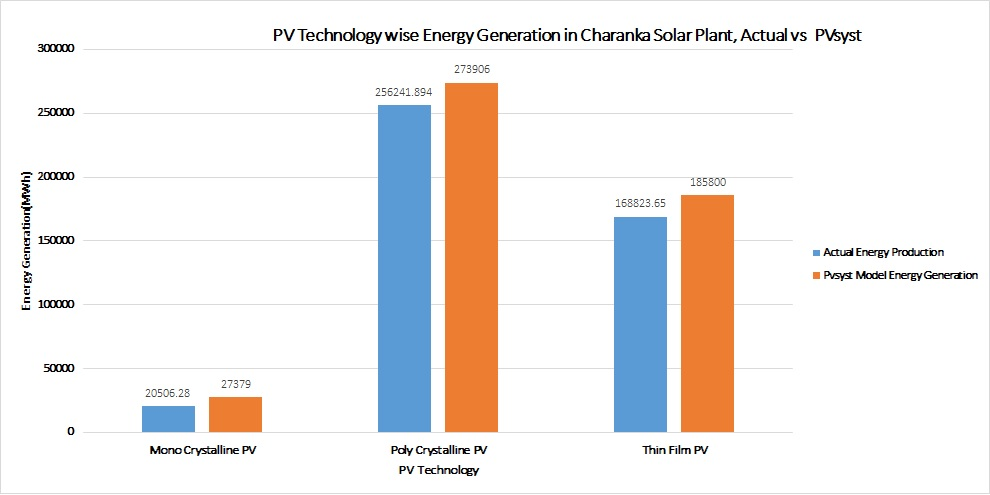
\includegraphics[scale=0.5]{Charanka2}
\caption{Charanka Solar Park PV Technology-Wise Energy Generation}
\label{figc2h7} %% to refer use, \ref{}
\end{figure}
\\
The Fig \ref{figc2h8} gives a good measure of performance of the different PV Technologies used in Charanka Solar Park, by measuring MWh/MW for all the plants using the same PV technology as a whole. We can see that with actual data Poly performs best and Mono performs the worst, however when we consider simulated values Mono performs best and Poly performs worst. 
\\

\begin{figure}[H]
\centering
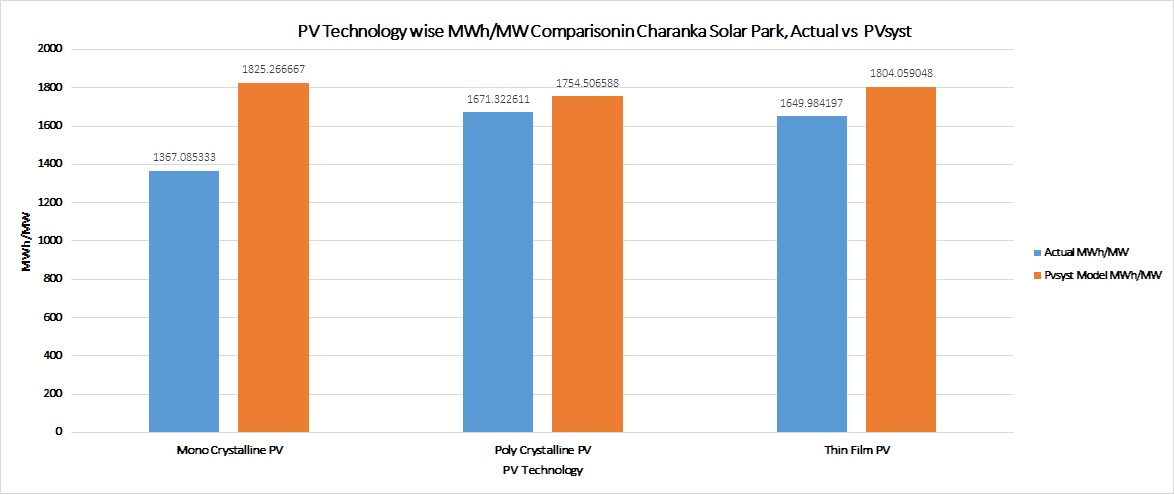
\includegraphics[scale=0.5]{Charanka1}
\caption{Charanka Solar Park PV Technology-Wise MWh/MW Comparison}
\label{figc2h8} %% to refer use, \ref{}
\end{figure}
\\
The Fig \ref{figc2h9} shows the PV Technology wise CUF comparison of Charanka Solar Park. We can observe that the the real and simulated values of CUF for Poly and Thin are approximately equal validating the PVsyst models, however even in this graph the simulated values for Mono are fairly larger than the real values; which indicates some modeling error.(most probably error could be the generalised weather data which PVsyst produces) 
\\
\begin{figure}[H]
\centering
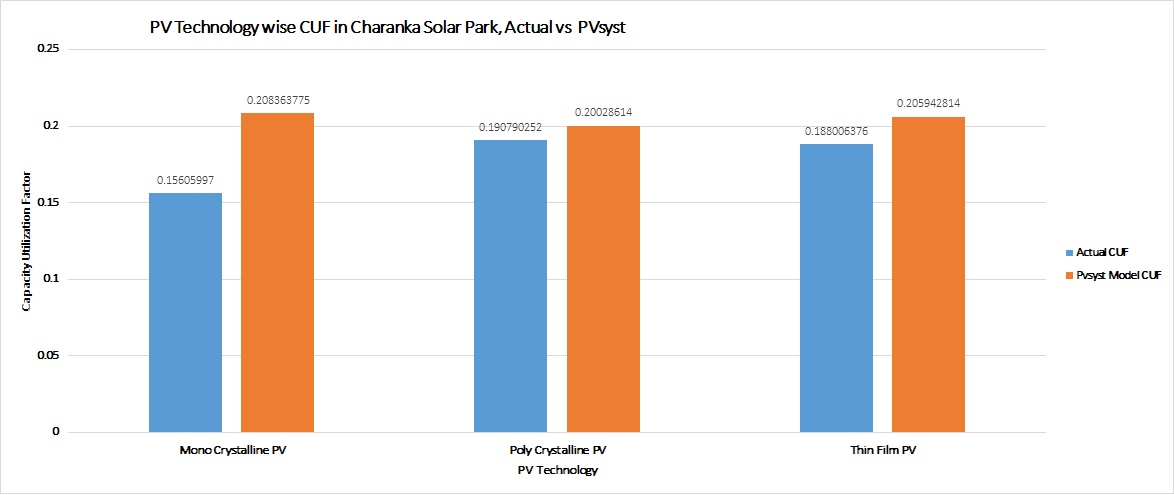
\includegraphics[scale=0.5]{Charanka3}
\caption{Charanka Solar Park PV Technology-Wise CUF Comparison}
\label{figc2h9} %% to refer use, \ref{}
\end{figure}

\section{Tracking Mechanism Performance Assessment using BACKBONE Plant Data}
\
\
\
\
The BACKBONE Enterprise LTD, 5MW Solar PV plant, in Kutch district is the only plant in whole of Gujarat to have a tracking mechanism. It uses a Single Axis (N-S axis)tracker system, details of which are given in Table \ref{tabc2h4}.
\\
\begin{table}[H]
  \centering
%%From Excet to LATEX Add-In  
    \begin{tabular}{|l|l|}
    \hline
    \textbf{Make} & SUNLINK  ViaSol Tracker \\
    \hline
    \textbf{Tracking Type (East/West)} & One-Axis Horizontal \\
    \hline
    \textbf{Tilt-Range} & +/- 45º (maximum) \\
    \hline
    \textbf{Backtracking} & Yes, Standard \\
    \hline
    \textbf{Sub-Array Rated Power} & Up to 1 MW dc \\
    \hline
    \textbf{Wind Load Capacity} & Up to 150 mph (35 mph stow) \\
    \hline
    \textbf{Time to Stow or Recover} & Less than 2 minutes \\
    \hline
    \textbf{Tracking Method} & Based on NASA time-and-location algorithm \\
    \hline
    \textbf{Drive Type} & Fluid Power \\
    \hline
    \textbf{Controller} & PLC controller utilizing industrial automation components \\
    \hline
    \textbf{Power Supply} & AC Supply from Auxiliary \\
    \hline
    \end{tabular}
%% All above Code is copied from Excel to LATEX Add-In 
    \caption{Tracker System Specifications}
    \label{tabc2h4}
\end{table}
\\
A model of the plant was created in PVsyst and simulated for Fixed Tilt (FT), Seasonal Tilt (ST), and Dual Axis Tracker (DA). We had the real values for the Single Axis Tracker (SA) and then compared them for analysis. The Table \ref{tabc2h5} shows the result of the PVsyst software simulation. 
\\

\begin{table}[H]
  \centering
     \caption{Tracker System Performance Comparison in PVsyst}
%%From Excet to LATEX Add-In  
    \begin{tabular}{|r|r|r|r|r|r|}
    \hline
    \textbf{} & \textbf{Actual} & \textbf{Fixed Tilt} & \textbf{Seasonal Tilt} & \textbf{N-S Axis} & \textbf{Dual-Axes} \\
    \hline
    \textbf{January} & 552.129 & 881.9 & 979.6 & 905   & 1174 \\
    \hline
    \textbf{February} & 642.4595 & 764.6 & 788.2 & 826   & 967 \\
    \hline
    \textbf{March} & 865.858 & 962.3 & 907.9 & 1144  & 1240 t\\
    \hline
    \textbf{April} & 916.5298 & 876   & 884   & 1143  & 1186 \\
    \hline
    \textbf{May} & 1044.885 & 863.4 & 883.2 & 1182  & 1209 \\
    \hline
    \textbf{June} & 599.0633 & 754.6 & 775.4 & 1020  & 1041 \\
    \hline
    \textbf{July} & 435.0063 & 581.8 & 595   & 730   & 740 \\
    \hline
    \textbf{August} & 425.8848 & 567.2 & 575.6 & 676   & 685 \\
    \hline
    \textbf{September} & 486.5465 & 741   & 741   & 874   & 920 \\
    \hline
    \textbf{October} & 550.0673 & 870.3 & 875.3 & 995   & 1136 \\
    \hline
    \textbf{November} & 452.825 & 797.9 & 864   & 825   & 1032 \\
    \hline
    \textbf{December} & 459.0528 & 825.4 & 932.2 & 812   & 1090 \\
    \hline
          &       &       &       &       &  \\
    \hline
    \textbf{Total Energy} & 7430.307 & 9486.4 & 9801.4 & 11132 & 12420 \\
    \hline
    \textbf{} &       &       &       &       &  \\
    \hline
    \textbf{MWh/MW} & 1486.061 & 1897.28 & 1960.28 & 2226.4 & 2484 \\
    \hline
          &       &       &       &       &  \\
    \hline
    \textbf{CUF} & 0.169642 & 0.216584 & 0.223776 & 0.254155 & 0.283562 \\
    \hline
    \end{tabular}%
    %% All above Code is copied from Excel to LATEX Add-In 
 
    \label{tabc2h5}%
\end{table}
\\
The Fig \ref{figc2h10} shows the monthly solar generations for different types of tracking mechanisms, and we see that the Dual Axis Tracker gives the best performance while Fixed Tilt gives the worst.
\\
\begin{figure}[H]
\centering
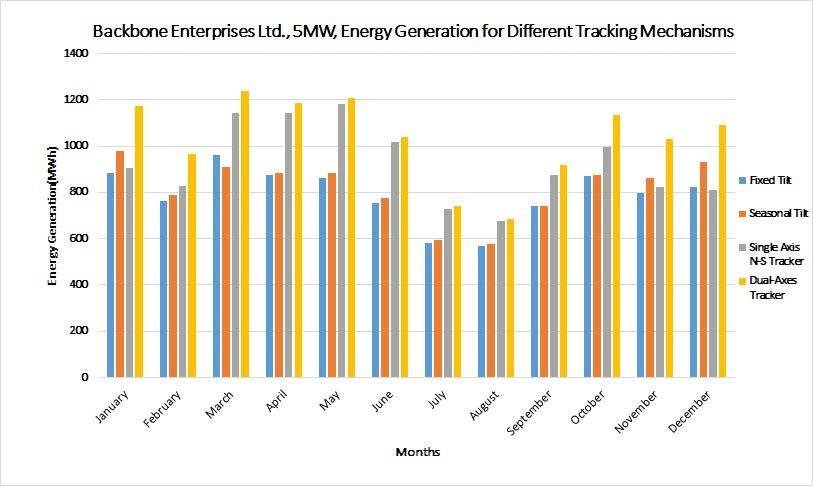
\includegraphics[scale=0.75]{Backbone1}
\caption{Monthly Solar Generation Comparison of different Tracking Mechanisms}
\label{figc2h10} %% to refer use, \ref{}
\end{figure}
\\
The Fig \ref{figc2h11} represents the CUF comparison of different tracking mechanisms. We observe that the performance of FT, ST, SA and DA improves in this same order.

\\

\begin{figure}[H]
\centering
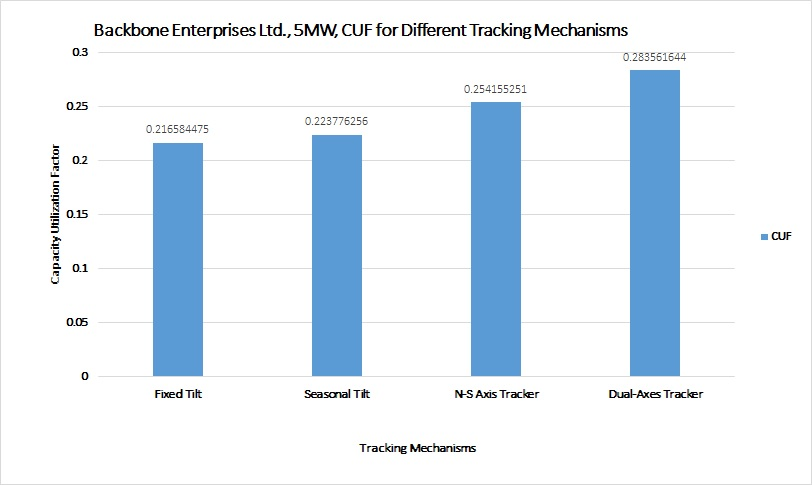
\includegraphics[scale=0.65]{Backbone3}
\caption{CUF Comparison of different Tracking Mechanisms}
\label{figc2h11} %% to refer use, \ref{}
\end{figure}

\newpage

\section{Generation and Weather Data Resources}
\
\
\
\
The historical generation data can be sort from SLDC, but it has a resolution of one day. To get higher resolution generation data of the order of days or hours, we have to take it directly from the Solar PV Plant SCADA system. But in most of the cases the plant logs only daily data for saving memory of the SCADA systems. I have collected generation data from the BACKBONE plant at a daily resolution.\\

Similarly historical weather data is available at Meteorological Institutes Website, they will usually have data at almost all resolutions, but you will have to pay for the data. Also, some web linked softwares like Meteonorm alsso provide quality weather data at almost all resolutions at a fee. However, the data obtained from these sources would not be cent percent accurate for the exact plant location. Hence, weather data logged into the plant SCADA system is the most reliable weather data we can ever get. I have received only Global Horizoltal Radiation (GHI) from Backbone as there is no provision for temperature and wind speed logging.





\chapter{Basics of Solar Energy}
%% Chapter 3 : Basics of Solar Energy

\section{Solar Radiation and Solar Spectrum}
\
\
\
\
Sun is the source of radiation. It is a thermonuclear furnace, where hydrogen atoms undergo fusion to become helium atoms. The mass lost in the process is converted into electromagnetic energy of the order of $3.8\times10^{20}$ MW. This energy is radiated outwards from the surface of he sun into space.\\

For the purpose of understanding the nature of absorption and emission of electromagnetic radiation by an object, we use a mathematical abstraction called a \textit{Blackbody}. It is the perfect emitter and absorber of radiation; which means that for a given area and temperature the blackbody will absorb  all radiation impinging on it, and emit more radiation per square unit area as compared to any other object. Moreover, no radiation is reflected or transmitted through a blackbody. The idea of the blackbody is credited to the German physicist Max Planck.\\

The wavelengths emitted by a blackbody are dependent on its temperature. This is described by the \textit{Planck's Law} given in eq (\ref{planck})

\begin{equation}
\label{planck}
E_{\lambda}=\frac{3.74\times10^{8}}{\lambda^{5} \left[\text{exp}\left( \frac{14,400}{\lambda T}\right)-1 \right]}
\end{equation}\\
where,\\
$ E_{\lambda} $ = Emissive power per unit area of a blackbody $ (W/m^{2}) $ \\
$ T $ = Absolute temperature of the body $ (K) $ \\
$ \lambda $ = Wavelength $ (\mu m) $ \\

The \textit{Stefan-Boltzman Law of Radiation} given in eq (\ref{stefbolt}) expresses the area under the Planck's curve between any two points, which represents the power emitted between those two wavelengths. This is called as the total emitted radiant power.

\begin{equation}
\label{stefbolt}
E = A \sigma T^{4}
\end{equation}\\
where,\\
$ E $ = Total blackbody emission rate $ (W) $ \\
$ A $ = Area of the body $ (m^{2}) $ \\
$ \sigma $ = Stefan-Boltzman constant $ (5.67\times10^{-8} W/m^{2}K^{4}) $ \\

One characteristic feature of the blackbody radiation curve is given by \textit{Wien's Displacement Rule} given in eq (\ref{wien}), which identifies the wavelength where the blackbody will emit maximum radiation.

\begin{equation}
\label{wien}
\lambda_{{max}}(\mu m)=\frac{2898}{T(K)}
\end{equation}\\
where,\\
$ \lambda_{max} $ = Wavelength at which blackbody emits maximum radiation $ (\mum) $ \\

The Fig \ref{figc3h1} shows the ideal blackbody Planck's curve at 5800 K, which is the surface temperature of the sun. The total area under this blackbody curve gives the solar insolation just outside the earth's atmosphere, which is approximately $1.37 \ \text{kW/m}^{2}$. The yellow part of the Fig \ref{figc3h1} shows the actual Solar Spectrum prior to entering earth's atmosphere, it approximately depicts the blackbody curve. The actual solar spectrum consists of:

\begin{enumerate}
\item Ultraviolet (UV) is 7\%
\item Visible is 47\%
\item Infrared (IR) is 46\%
\end{enumerate}

\begin{figure}[H]
\centering
\includegraphics[scale=1]{SolarSpec}
\caption{Solar Spectrum [5]}
\label{figc3h1} %% to refer use, \ref{}
\end{figure}

Also, the red part of Fig \ref{figc3h1} shows the Solar Spectrum (terrestrial spectrum) after passing through the earth's atmosphere, where it undergoes various stages of absorption. Hence, the available solar energy on the surface of the earth is lesser than that available outside the atmosphere. 

\section{Photovoltaic Cell}
\
\
\
\
The photovoltaic cell is physically equivalent to a p-n junction diode shown in Fig (\ref{figc3h2}). A p-n junction diode consists of two types of semiconducting materials, which are n-type and p-type materials. The n-type material has been doped with a valency +5 element atoms, which donates the extra electron to the lattice which is free to move within the crystal lattice formed by the valency 4 Silicon atoms and the donor atoms; hence, the n-type materials have free electrons. Whereas, for creating a p-type material valency +3 element atoms, which creates a hole in the crystal lattice which can readily accept a free moving electron; hence, the p-type materials have positively charged holes (lack of an electron can be mathematically termed as a positive charge). However, the net charge of both the n and p type materials is neutral.

\begin{figure}[H]
\centering
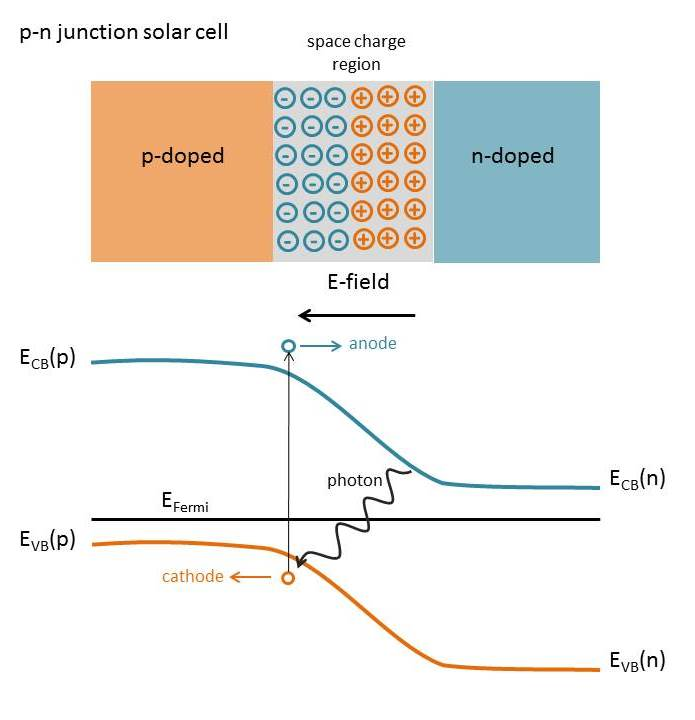
\includegraphics[scale=0.5]{pn-junction}
\caption{PN- Junction Diode}
\label{figc3h2} %% to refer use, \ref{}
\end{figure}

A pn-junction diode is formed by joining a p-type material with an n-type material. Now, at the junction of the diode the mobile electrons from the n region and the mobile holes from the p region of the diode drift by diffusion across the junction, leaving behind static positive charges and negative charges in the n region and p region of the diode respectively. These immobile charges create  a static electric field which opposes the diffusion of mobile electron and holes (also called charged carriers). The diffusion process continues till the electric field increases so much so that it restricts all further  diffusion of the charged carriers across the junction. This region of immobile charges at the junction is called the depletion region (depleted of mobile charged carriers). The width of the depletion region is about 1 $\mu \text{m} $ and the voltage across it is about 1 V; hence, electric field strength is about 10,000 V/cm. The Fig (\ref{diode12}) shows the symbol characteristics of a pn-junction diode.

\begin{figure}[H]
\centering
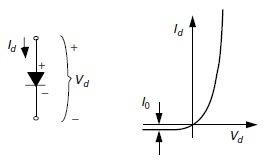
\includegraphics[scale=1]{diode1}
\caption{PN Juction Diode Symbol and Characteristics [5]}
\label{diode12} %% to refer use, \ref{}
\end{figure}

There are two modes of operation of a p-n junction diode. Firstly, the forward conduction mode, where an external positive voltage is applied across p-side and n-side (the external voltage cancels the effect of electric feild developed by the depletion region and allows for further diffusion reducing the width of the depletion region), in this mode the diode conducts very well offering least resistance. But, when a the voltage polarity across the pn-junction diode is reversed it blocks the flow of current offering maximum resistance, this mode of operation is called the reverse bias. Still a small amount of current flows due to thermally generated carriers, this current is called the reverse saturation current. The voltage-current characteristics for the pn-junction diode is described by the Shockley diode equation given by eq (\ref{diode}) 

\begin{equation}
\label{diode}
I_{d} = I_{0}( e^{qV_{d}/kT}-1)
\end{equation}\\
where,\\
$ I_{d} $ = Diode Current $ (A) $ \\
$ I_{0} $ = Reverse saturation current $ (A) $ \\
$ q $ = Electron charge $ (1.602\times10^{-19} C) $ \\
$ V_{d} $ = Voltage across diose terminals frm p-side to n-side $ (V) $ \\
$ k $ = Boltzman's constant $ (1.381\times10^{-23} J/K) $ \\

The Fig (\ref{d2}) shows the operation principle of a photovoltaic cell. When a pn-junction diode is exposed to sunlight, owing to the photo-electric effect photons of sunlight will be absorbed and electron-hole pairs will be formed.

\begin{figure}[H]
\centering
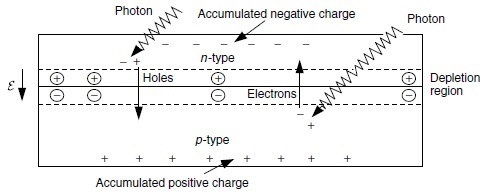
\includegraphics[scale=1]{pv8}
\caption{PN-Junction Diode as a Photovoltaic Cell [5]}
\label{d2} %% to refer use, \ref{}
\end{figure}

If these mobile charge carriers reach near the depletion layer, the electric field in the depletion layer will push the holes to the p-side and electrons to the n-side. Hence, holes will accumulate in the p-side and electrons in the n-side of the pn-junction diode. Now, if electrical contacts are attached to the pn-junction diode ends, conventional current will from p-side (electrons flow from the n-side) into the wire, through the load and back to the n-side, thus completing a circuit.\\

A simple model of a photovoltaic cell consists of a pn-junction diode in parallel with an ideal current source shown in Fig (\ref{p1}), where the ideal current source produces current in direct proportion to the amount of solar flux incident on it.

\begin{figure}[H]
\centering
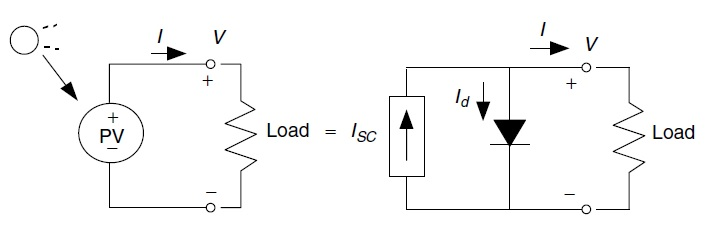
\includegraphics[scale=1]{pv9}
\caption{Simple Equivalent circuit of a Photovoltaic Cell [5]}
\label{p1} %% to refer use, \ref{}
\end{figure}

From Fig (\ref{pv9}) we can write the voltage and current equations for the PV cell as,

\begin{equation}
\label{pv1}
I = I_{SC}-I_{d}
\end{equation}\\
where,\\
$ I $ = Current output from PV Cell $ (A) $ \\
$ I_{SC} $ = Short circuit current of PV Cell $ (A) $ \\

Substituting the value of $I_{d}$ in above equation we get,

\begin{equation}
\label{pv2}
I = I_{SC}-I_{0} \left(e^{qV/kT}-1 \right )
\end{equation}

Where, $I_{SC}$ is the short circuit current, i.e. the current measured when the p-side and n-side are shorted, which means $V=0$, and $I$ is the load current.\\

Conversely, when the leads from the PV cell are kept open, no current flows i.e. $I=0$, the voltage measured is called as open-circuit voltage $(V_{OC})$, which is given by the following equation,

\begin{equation}
\label{pv3}
V_{OC} = \frac{kT}{q}\ln \left (\frac{I_{SC}}{I_{0}}+1\right )
\end{equation}\\
where,\\
$ V_{OC} $ = Open circuit voltage of PV Cell $ (V) $\\

The eq (\ref{pv2},\ref{pv3}) at $25^{\circ} \text{C}$ are given by the following equations,

\begin{equation}
\label{pv4}
I = I_{SC}-I_{0} \left(e^{38.9V}-1 \right )
\end{equation}

\begin{equation}
\label{pv5}
V_{OC} = 0.0257\ln \left (\frac{I_{SC}}{I_{0}}+1\right )
\end{equation} 



\subsection{PV Cell Model with Shunt Resistance}
\
\
\
\
A more accurate model of PV cell is developed when a resistance is added in parralel to the pn-junction diode as shown in Fig (\ref{fig3h4})

\begin{figure}[H]
\centering
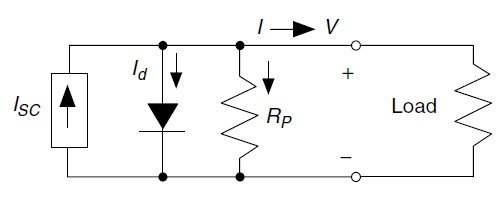
\includegraphics[scale=1]{PVmo}
\caption{PV Cell Model With Shunt Resistance [5]}
\label{figc3h4} %% to refer use, \ref{}
\end{figure}

This model describes the behaviour of a PV cell in a string of PV cell. If we consider that one of the PV cells in the string is shaded, then it will not produce current, moreover the pn-junction diode pertaining to that cell will be reverse biased and no current will not allow any flow of current. This will cause the entire current output from the string of PV cells to be reduced to zero, and no power is delivered to the load according to the simple equivalent model. But, in reality this is not the case and power though reduced in amount is delivered to the load even during shading. Hence, the voltage and current characteristics of a PV cell model with parallel resistance $R_{P}$ is given as follows,

\begin{equation}
\label{pv6}
I = (I_{SC}-I_{d})-\frac{V}{R_{P}}
\end{equation}\\
where,\\
$ V $ = Voltage at output of PV Cell $ (V) $ \\
$ R_{P} $ = Parallel resistance of the PV Cell $ (\Omega) $ 

\begin{figure}[H]
\centering
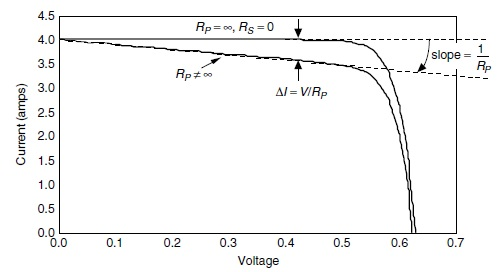
\includegraphics[scale=1]{pv1}
\caption{Effect of Parallel Resistance on I-V Curve [5]}
\label{figc3h111} %% to refer use, \ref{}
\end{figure}

The Fig (\ref{figc3h111]) shows the effect of parallel resistance on the I-V characteristics of the PV cell. It can be observed that the parallel resistance causes the load current for the simple model to be decreased by $V/R^{P}$.

\subsection{PV Cell Model with Series Resistance}
\
\
\
\
There is some intrinsic resistance of the semiconductor and also the contact resistance of the bond between the the wires and the cell leads. This resistance is called the series resistance ($R_{S}$), as it reduces the voltage availabe at the load terminals.
Hence, an accurate model of a PV cell should consinder $R_{S}$ as shown in Fig (\re{figc3h3})

\begin{figure}[H]
\centering
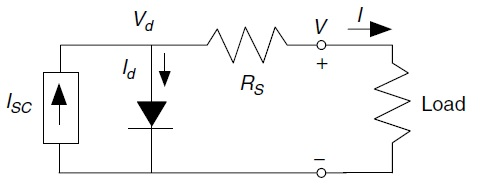
\includegraphics[scale=1]{PVmm}
\caption{PV Cell Model with Series Resistance [5]}
\label{figc3h3} %% to refer use, \ref{}
\end{figure}

The voltage and current characteristics of the PV cell with a series resistance are given by the following equations,

\begin{equation}
\label{pv7}
V_{d}=V+I.R_{S}
\end{equation}\\
where,\\
$ R_{S} $ = Series resistance of the PV Cell $ (\Omega) $ 

\begin{equation}
\label{pv8}
I = I_{SC}-I_{0} \left\{\text{exp}\left[\frac{q(V+I.R_{S})}{kT} \right]-1 \right\}
\end{equation}

\begin{figure}[H]
\centering
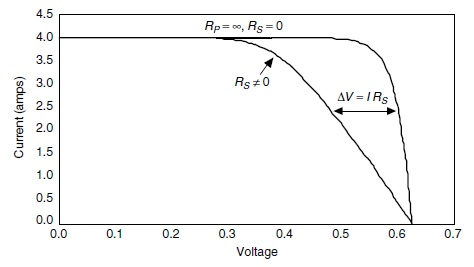
\includegraphics[scale=1]{pv2}
\caption{Effect of Series Resistance on I-V Curve [5]}
\label{figc3h222} %% to refer use, \ref{}
\end{figure}

The Fig (\ref{figc3h222}) shows the effect of series resistance on the I-V curve of the PV cell. It can be observed that the series resistance reduces the voltage available at the load by the factor of $IR_{S}$.

\subsection{Complete PV Cell Model}
\
\
\
\
The complete PV cell model as shown in Fig (\ref{figc3h333}) includes the both the parallel as well as the series resistance. This model of the PV cell is highly accurate.

\begin{figure}[H]
\centering
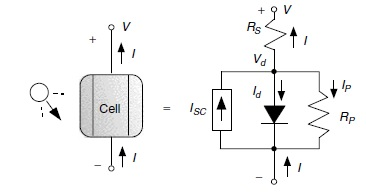
\includegraphics[scale=1]{pv3}
\caption{Complete Model of PV Cell [5]}
\label{figc3h333} %% to refer use, \ref{}
\end{figure}

The load current equation for this model is given by the following equation,

\begin{equation}
\label{pv10}
I_{SC}=I+I_{d}+I_{P}
\end{equation}\\
where,\\
$ I_{P} $ = Current in the parallel branch of the PV Cell $ (A) $\\ 

The effect of series resistance is given by the following equation,

\begin{equation}
\label{pv11}
V=V_{d}-IR_{S}
\end{equation}

The combined effect of the series and parallel resistances is given in the following equation, 

\begin{equation}
\label{pv9}
I = I_{SC}-I_{0} \left\{\text{exp}\left[\frac{q(V+I.R_{S})}{kT} \right]-1 \right\}-\left(\frac{V+I.R_{S}}{R_{P}}\right)
\end{equation}

\subsection{I-V Curve}
\
\
\
\
Fig (\ref{figc3h5}) shows the I-V curve of the PV cell. The I-V curve helps us identify the key parameters of the PV cell. On the horizontal axis we find open-circuit voltage $(V_{OC})$ when current is zero, and on the vertical axis we find the short-circuit current $(I_{SC})$ when the voltage is zero; at both these points the power delivered by the PV cell is zero as either voltage or current are zero $(P=VI)$.

\begin{figure}[H]
\centering
\includegraphics[scale=0.5]{PVivp [5]}
\caption{PV Cell I-V Curve}
\label{figc3h5} %% to refer use, \ref{}
\end{figure}

The maximum power delivered is obtained at the knee of the I-V curve, the point is called as the maximum power point (MPP). The voltage and current at the MPP are represented as $V_{m}$ and $I_{m}$. The I-V curve summarizes the entire performance characteristic of the PV cell. Any other point on the I-V curve is represented as $V_{R}$ and $I_{R}$.

\subsection{Effect of Insolation and Temperature on I-V Curve}
\
\
\
\
\
The Fig (\ref{figc3h6}) shows the PV cell curves for two different values of insolation. We observe that the short-circuit current is directly proportional to insolation, and it changes linearly with insolation. But, the open-circuit voltage is inversely proportional to the insolation, and it changes modestly with insolation as it follows a logarithmic relationship. Hence, as insolation increases the power output from the PV cell increases.

\begin{figure}[H]
\centering
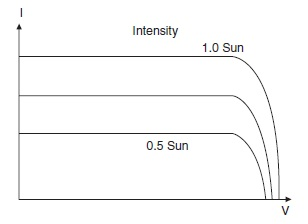
\includegraphics[scale=1]{PVinso}
\caption{Effect of Insolation on I-V Curve [5]}
\label{figc3h6} %% to refer use, \ref{}
\end{figure}

The Fig (\ref{figc3h7}) shows the PV cell curves for two different values of temperature. We observe that as temperature increases the open-circuit voltage decreases considerably, while the short-circuit current increases very slightly. Hence, the power output of PV cell increases on a clear and cold day. 

\begin{figure}[H]
\centering
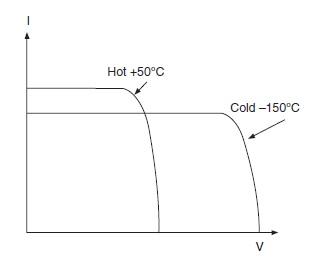
\includegraphics[scale=1]{PVtemp}
\caption{Effect of Temperature on I-V Curve [5]}
\label{figc3h7} %% to refer use, \ref{}
\end{figure}

The cell temperature depends not only on ambient temperature; but also on insolation as small fraction of insolation hitting the cell is converted to electricity, and the rest is converted to heat. Hence, manufacturers of the PV cells provide clients with a normal operating cell temperature (NOCT); it is the temperature in the cell when the ambient temperature is $20^{\circ} \text{C}}$, solar irradiance is $0.8 \  \text{kW/m}^{2}$, and windspeed is 1 m/s. This value helps in accounting the changes in the PV cell performance with temperature. The cell temperature can be calculated using the following equation, 

\begin{equation}
\label{tefpv}
T_{{cell}}=T_{{amb}}+\left(\frac{NOCT-20^{\circ}}{0.8}\right)
.\ S
\end{equation}

\newpage

\section{Cells, Modules and Arrays}
\
\
\
\
The individual cell with its small voltage of 0.5 V cannot be used alone for producing power for everyday applications. Hence, to increase the power output, a number of cells are connected together in series and parallel to form a module, which is encased in tough weather-resistant packages. Usually 36 cells are connected in series to give a module with voltage of 12 V and the number of parallel strings can be adjusted according to the amount of power to be generated from a module. Also, there are large modules with 72 cell connected in series giving a voltage of 72 V.

\begin{figure}[H]
\centering
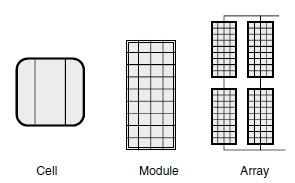
\includegraphics[scale=1]{pv4}
\caption{PV - Cell, Module and Array [5]}
\label{figc3h444} %% to refer use, \ref{}
\end{figure}

To increase the power generation capacity further, modules can be connected in series to increase voltage and a number of similar parallel strings can be connected to increase the current. Such a combination of modules is called as an array.

The eq (\ref{mod1}) gives the voltage equation for a module, where $n$ is the number of cells connected in series.

\begin{equation}
\label{mod1}
V_{{module}}=n(V_{d}-IR_{S})
\end{equation}\\
where,\\
$ V_{{module} $ = Total voltage of a PV Module $ (V) $ \\
$ n $ = Total number of PV Cells in one string in the PV Module  \\

From Fig (\ref{figc3h555}) we observe that as the number of cells in series in a module increase, the open-circuit voltage increases. But, the short-circuit current remains the same, hence the MPP has horizontal movement; and power output of the module increases

\begin{figure}[H]
\centering
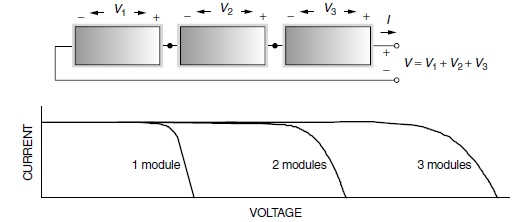
\includegraphics[scale=1]{pv5}
\caption{Effect of Series connected modules on I-V Curve [5]}
\label{figc3h555} %% to refer use, \ref{}
\end{figure}

The eq (\ref{mod2}) gives the current equation for a module, where $p$ is the number of strings in the module.

\begin{equation}
\label{mod2}
I_{{module}}=p(I_{SC}-I_{d}-I_{P})
\end{equation}\\
where,\\
$ I_{{module}} $ = Total current of the PV Module $ (A) $ \\
$ p $ = Total number of parallel strings of PV Cells in the PV Module\\

From Fig (\ref{figc3h666}) we observe that as the number of strings in a module increase, the short-circuit current increases. But, the open-circuit voltage remains the same, hence the MPP has a vertical movement; and power output of the module increases.

\begin{figure}[H]
\centering
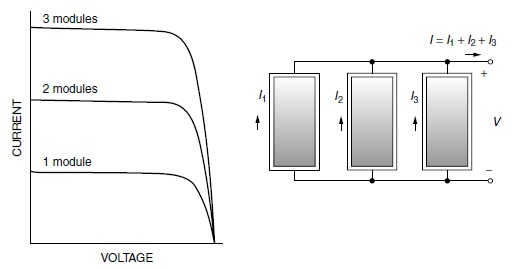
\includegraphics[scale=1]{pv6}
\caption{Effect of Parallel connected modules on I-V Curve [5]}
\label{figc3h666} %% to refer use, \ref{}
\end{figure}

\newpage

\section{Effect of Shading on PV Modules}
\
\
\
\
To understand the concept of shading in the PV cells let us consider the Fig (\ref{figc3h888}). It shows a string of $n$ cells, figure on the left shows condition when all the cells are in the sun. This will give us the usual behaviour of the PV module, where the major component of the current from the preceding cells will pass through the $I_{SC}$ current source branch.

\begin{figure}[H]
\centering
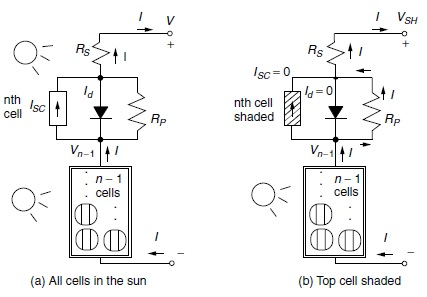
\includegraphics[scale=1]{shading1}
\caption{PV module with \textit{n} Cells - top cell in sun, or in shade [5]}
\label{figc3h888} %% to refer use, \ref{}
\end{figure}

But, the figure on the right shows the condition when one cell from the string is shaded (it does not produce current). Here we can see that the path taken by the current from the preceding cells in the string will have to pass through the branch of parallel resistance, which causes a large voltage drop as the value of parallel resistance is high. This drop in voltage reduces the power output of the module severely.\\

The output voltage $(V_SH)$ of the $n$ celled shaded module is given in the following equation,

\begin{equation}
\label{shade1}
V_{SH}=V_{n-1}-I(R_{P}+R_{S})
\end{equation}

Output voltage across $n-1$ cells $(V_{n-1})$ if $V$ is the output voltage of $n$ cells is given by, 

\begin{equation}
\label{shade2}
V_{n-1}=\left(\frac{n-1}{n}\right)V
\end{equation}\\
where,\\
$ n $ = Total number of cells ahaded $  $ \\
$ V_{n-1} $ = Output voltage across $ n-1 $ cells $ (V) $ \\
$ \triangledown V $ = Voltage drop caused by shaded cell $ (V}) $ 

Putting eq (\ref{shade2}) in eq (\ref{shade1}), we get;

\begin{equation}
\label{shade3}
V_{SH}=\left(\frac{n-1}{n}\right)V-I(R_{P}+R_{S})
\end{equation}\\
where,\\
$ V_{SH} $ = Output voltage of a $\text{n celled}$ shaded module $ (V) $ \\

Hence, the drop in voltage $(\triangledown)V$ at any given current $I$, caused by shaded cell is given by the following equation,

\begin{equation}
\label{shade4}
\triangledown V=\frac{V}{n}-I(R_{P}+R_{S})
\end{equation}\\
where,\\
$ \triangledown V $ = Voltage drop caused by shaded cell $ (V}) $ \\

The above equation can be modified as follows, as parallel resistance is very large as compared to the series resistance. Hence, neglecting the effect of series resistance, we get the following equation, 

\begin{equation}
\label{shade4}
\triangledown V=\frac{V}{n}-IR_{P}
\end{equation}

The Fig (\ref{figc3h999}) shows the comparison of I-V curves for an un-shaded and a shaded module. We can observe that in the module with shading both the short-circuit current and open-circuit voltage are reduced and the curve assumes a linear shape, which drastically reduces the power output from the module.

\begin{figure}[H]
\centering
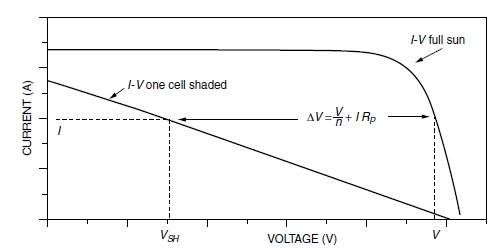
\includegraphics[scale=1]{shading2}
\caption{Effect of shading one cell in \textit{n} cell module [5]}
\label{figc3h999} %% to refer use, \ref{}
\end{figure}

\newpage

\subsection{Bypass Diode}
\
\
\
\
In order to overcome the problem of shading, bypass diodes are used as shown in Fig (\ref{figc3h100}). The figure on the left in Fig (\ref{figc3h100}) shows a PV cell which is un-shaded, here the bypass diode will be reverse biased as the PV ell produces reverse voltage across the bypass diode; hence, no current follow through the bypass diode when the cell is un-shaded.

\begin{figure}[H]
\centering
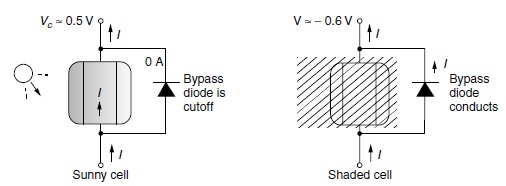
\includegraphics[scale=1]{bydiode1}
\caption{Mitigation of shading problem with Bypass Diode - In sunny cell bypass diode is cut-off, in shaded cell it conducts [5]}
\label{figc3h100} %% to refer use, \ref{}
\end{figure}

The figure in right in Fig (\ref{figc3h100}) shows a shaded PV cell with a bypass diode. As the cell is shaded the output voltage of the cell is reduced drastically, moreover the current from the preceding cells rather than passing through the parallel resistance of the shaded cell causing large voltage drop flows through the bypass diode as it gets forward biased. Hence, the bypass diode reduces the amount of voltage reduced due to shading(voltage drop in the bypass diode is about 0.5 V).

\begin{figure}[H]
\centering
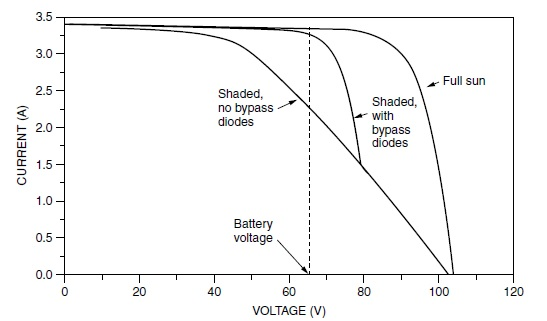
\includegraphics[scale=1]{bydiode2}
\caption{Effect of Bypass Diode on I-V Curve [5]}
\label{figc3h190} %% to refer use, \ref{}
\end{figure}

The Fig (\ref{figc3h190}) shows the comparison of I-V curves for shaded cell, un-shaded cell and shaded cell with bypass diode. We observe that the bypass diode improves the performance of the shaded cell by increasing the MPP point; however, it does not completely eliminate the effect of shading.

\subsection{Blocking Diode}
\
\
\
\
Blocking diodes as shown in Fig (\ref{figc3h200}) are connected at the top of each string of an array. The blocking diode will conduct only when the source of current is the string as it is in forward biased mode. But, when the string malfunctions or is shaded it acts as a load and draws current, the blocking diode becomes reverse biased and prevents any flow of current to the string. Hence a blocking diode helps improve the performance of a PV array.

\begin{figure}[H]
\centering
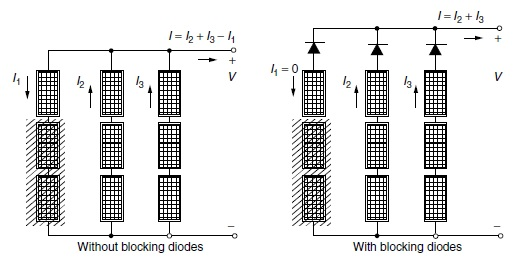
\includegraphics[scale=0.75]{bldiode1}
\caption{Blocking Diode prevents reverse flow of current through PV modules [5]}
\label{figc3h200} %% to refer use, \ref{}
\end{figure}

\newpage

\section{Results of PV-IV Curve App}
\
\
\
\
The Table (\ref{tabc3h1})gives the information of the different PV modules, which are used to simulate P-V and I-V curves from the PV-IV Curve App.

\begin{table}[htbp]
  \centering
  \caption{PV Module Information}
    \begin{tabular}{|l|c|c|c|c|}
    \hline
    \textbf{TYPE} & \textbf{Poly} & \textbf{Mono} & \textbf{Cdte} & \textbf{A-si} \bigstrut\\
    \hline
    \textbf{MAKE} & Lanco & Lanco & First Solar & Du-Pont \bigstrut\\
    \hline
    \textbf{Crys/TF} & Crys & Crys & TF & TF \bigstrut\\
    \hline
    \textbf{Pmpp (W)} & 235 & 250 & 85 & 107 \bigstrut\\
    \hline
    \textbf{Vmpp (V)} & 29.56 & 31.15 & 46.4 & 74 \bigstrut\\
    \hline
    \textbf{Impp (A)} & 7.95 & 8.034 & 1.83 & 1.44 \bigstrut\\
    \hline
    \textbf{Voc (V)} & 37.17 & 38.04 & 60.5 & 99 \bigstrut\\
    \hline
    \textbf{Isc (A)} & 8.4 & 8.712 & 1.94 & 1.81 \bigstrut\\
    \hline
    \textbf{Kv} & -0.31 & -0.33 & -0.27 & -0.3 \bigstrut\\
    \hline
    \textbf{Ki} & 0.06 & 0.036 & 0.04 & 0.09 \bigstrut\\
    \hline
    \textbf{Kp} & -0.43 & -0.47 & -0.25 & -0.25 \bigstrut\\
    \hline
    \end{tabular}%
  \label{tabc3h1}%
\end{table}%
\\
Where Crys-Crystalline, TF-Thin Film, mmp-Maximum Power Point, oc-Open Circuit, sc-Short Circuit, P-Power, V-Voltage, I-Current and Kv, Ki, Kp are the temperature co-efficients of voltage, current and power respectively.\\

The PV and IV curves are plotted at different temperatures (-25, 0, 25, 50 and 75 ºC) and different irradiances ( 200, 400, 600, 800 and 1000 W/m^{2}) are as follows,

\begin{figure}[H]
\centering
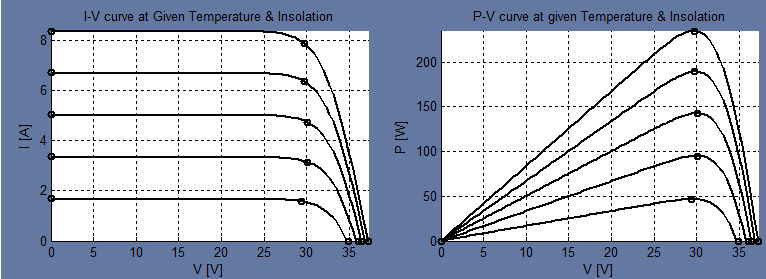
\includegraphics[scale=0.5]{Poly_Irradiance}
\caption{Polycrystalline Solar PV module I-V and P-V Curves at different Irradiances}
\label{figc3h15} %% to refer use, \ref{}
\end{figure}

\begin{figure}[H]
\centering
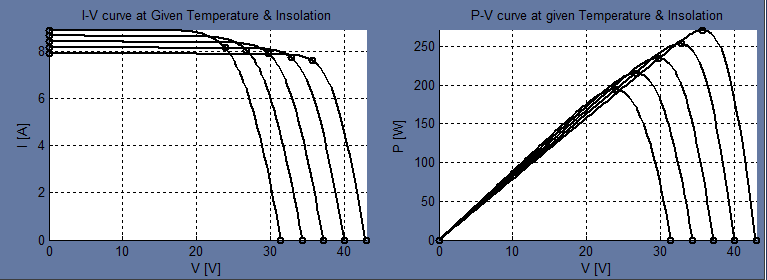
\includegraphics[scale=0.5]{Poly_Temperature}
\caption{Polycrystalline Solar PV module I-V and P-V Curves at different Temperatures}
\label{figc3h16} %% to refer use, \ref{}
\end{figure}

\begin{figure}[H]
\centering
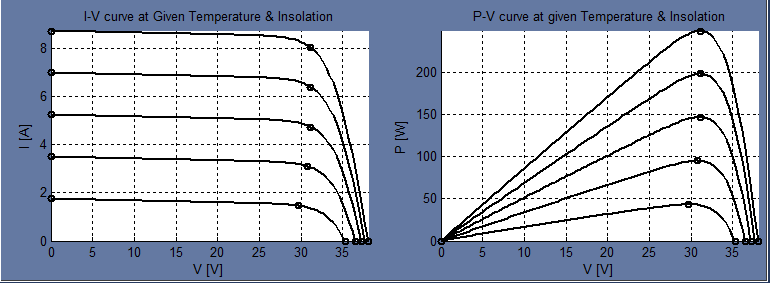
\includegraphics[scale=0.5]{Mono_Irradiance}
\caption{Monocrystalline Solar PV module I-V and P-V Curves at different Irradiances}
\label{figc3h17} %% to refer use, \ref{}
\end{figure}

\begin{figure}[H]
\centering
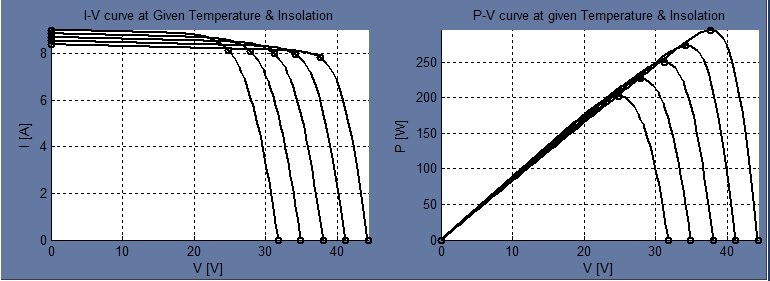
\includegraphics[scale=0.5]{Mono_Temperature}
\caption{Monocrystalline Solar PV module I-V and P-V Curves at different Temperatures}
\label{figc3h18} %% to refer use, \ref{}
\end{figure}

\begin{figure}[H]
\centering
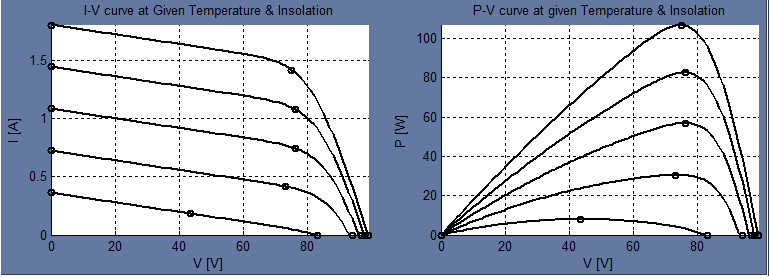
\includegraphics[scale=0.5]{A-si_Irradiance}
\caption{A-Si Thin Film Solar PV module I-V and P-V Curves at different Irradiances}
\label{figc3h19} %% to refer use, \ref{}
\end{figure}

\begin{figure}[H]
\centering
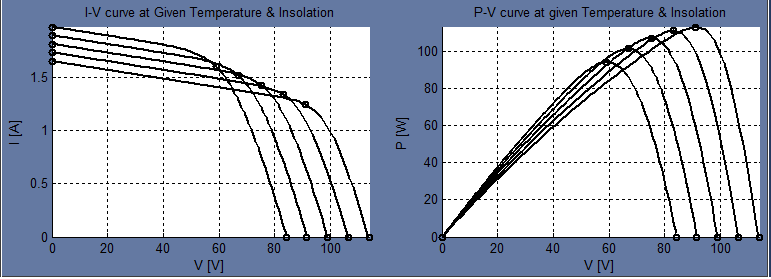
\includegraphics[scale=0.5]{A-si_Temperature}
\caption{A-Si Thin Film Solar PV module I-V and P-V Curves at different Temperatures}
\label{figc3h20} %% to refer use, \ref{}
\end{figure}

\begin{figure}[H]
\centering
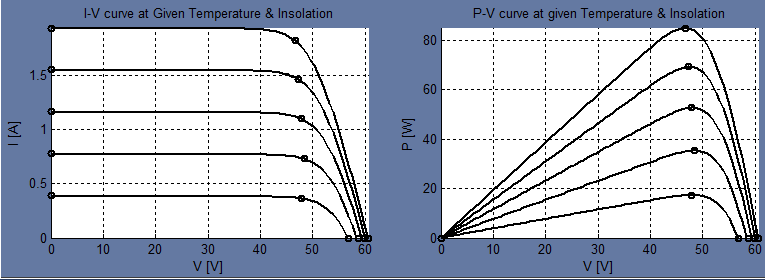
\includegraphics[scale=0.5]{CDTE_Irradiance}
\caption{CDTE Thin Film Solar PV module I-V and P-V Curves at different Irradiances}
\label{figc3h21} %% to refer use, \ref{}
\end{figure}

\begin{figure}[H]
\centering
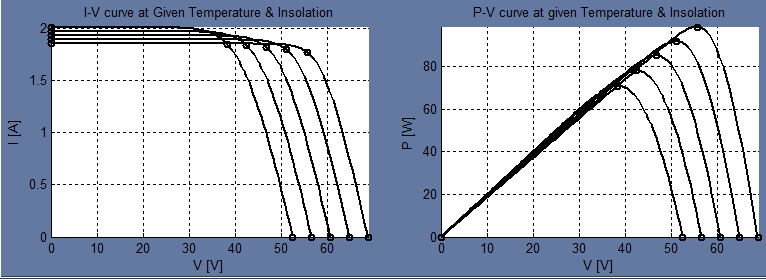
\includegraphics[scale=0.5]{CDTE_Temperature}
\caption{CDTE Thin Film Solar PV module I-V and P-V Curves at different Temperatures}
\label{figc3h22} %% to refer use, \ref{}
\end{figure}
The effect of decreasing irradiance with temperature at kept constant at 25ºC can be observed in Fig (\ref{figc3h15}, \ref{figc3h17}, \ref{figc3h19}, \ref{figc3h21}). It is clearly seen that the photovoltaic module current output and power are directly proportional to the irradiance level, however the module voltage increases by very small values with decreasing irradiance levels. This concurs with the theory that module current is a direct function of the solar irradiance.\\

The effect of increasing temperature with irradiance level kept constant at 1000 W/m2 can be observed in Fig (\ref{figc3h16}, \ref{figc3h18}, \ref{figc3h20}, \ref{figc3h22}). It is clearly seen that the module voltage and power output are inversely proportional to the temperature, however the module current increases very slightly with increase in temperature. This concurs with theory that diode voltage is inversely proportional to temperature.

\begin{figure}[H]
\centering
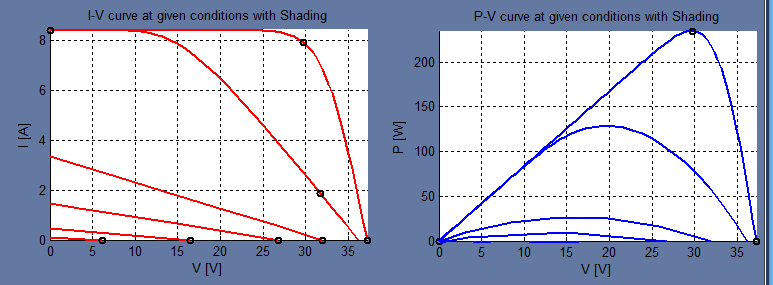
\includegraphics[scale=0.5]{Poly_Shading_WithoutByPassDiode}
\caption{Polycrystalline Solar PV moduleP-V and I-V curves for Shading without Bypass Diode and at different number of shaded cells}
\label{figc3h23} %% to refer use, \ref{}
\end{figure}

\begin{figure}[H]
\centering
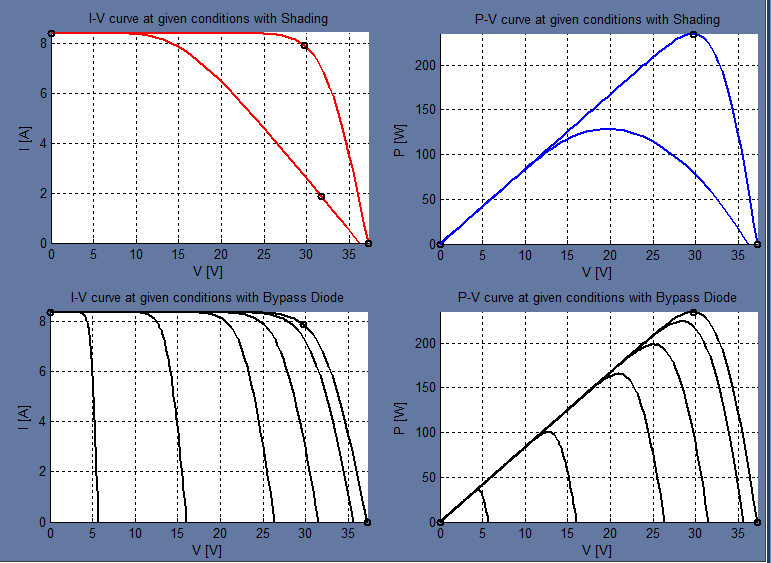
\includegraphics[scale=0.5]{Poly_Shading_With_ByPassDiode}
\caption{Polycrystalline Solar PV moduleP-V and I-V curves for Shading with Bypass Diode and at different number of shaded cells}
\label{figc3h24} %% to refer use, \ref{}
\end{figure}

In Fig (\ref{figc3h23}) we can observe that as the number of single cells within a module being shaded increase, both the PV and IV curves start becoming flat. Hence, shading of even a single cell almost reduces the module power by half and this can be attributed to the voltage loss in the series and parallel equivalent resistances due to the flow of the module output current.\\

To mitigate the shading effect, bypass diodes are used, which allow for alternative path to the current to flow which would have otherwise flowed through Rp and Rs causing large voltage drops, which consequently causes large reductions in output power. Ideally for the best shading effect mitigation, each cell within a module should be supplied with its own bypass diode, but as this would be escalate the cost and manufacturing complexity; hence optimal number of cell per bypass diodes have to selected. In Fig (\ref{figc3h24}) it can be observed that as the number of cell per bypass diode increase the performance of the module deteriorates.\\

\newpage

\section{Variables Affecting Solar PV Cell Output}
\
\
\
\
From the discussions in the previous sections, it is clear that the performance of a PV Cell depends on the following four variable;

\begin{enumerate}
\item Insolation
\item Temperature
\item Wind Speed
\item Cloud Cover
\end{enumerate}

The Fig (\ref{mfigc3h1}) shows pictures of some instruments which help in measuring the above mentioned variables.

\begin{figure}[H]
    \centering
    \begin{subfigure}[b]{0.45\textwidth}
       \centering
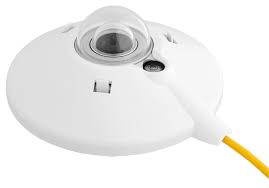
\includegraphics[scale=0.5]{Pyranometer}
\caption{Pyranometer}
\label{figc3h8}
    \end{subfigure}
    \hfill%% Fill Horizontal Space between two Figures
        \begin{subfigure}[b]{0.45\textwidth}
       \centering
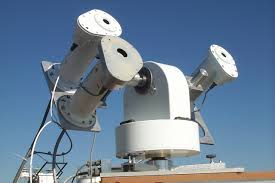
\includegraphics[scale=0.5]{Pyrheliometer}
\caption{Pyrheliometer}
\label{figc3h9} %% to refer use, \ref{}
    \end{subfigure}
    \caption{}
    \label{}
\end{figure} 
   

\begin{figure}[H]
    \centering
    \begin{subfigure}[b]{0.45\textwidth}
\centering
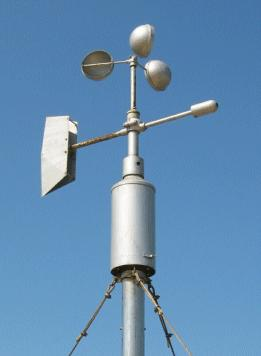
\includegraphics[scale=0.5]{Anemometer}
\caption{Anemometer}
\label{figc3h10} %% to refer use, \ref{}
    \end{subfigure}
    \hfill%% Fill Horizontal Space between two Figures
        \begin{subfigure}[b]{0.45\textwidth}
\centering
\includegraphics[scale=0.5]{Temperature}
\caption{TEmperature Sensor}
\label{figc3h11} %% to refer use, \ref{}
    \end{subfigure}
    \caption{Weather Variables Measurement Instruments}
    \label{mfigc3h1}
\end{figure}  

The Fig (\ref{figc3h8}) shows a Pyranometer, it mmeasures the Global Horizontal Irradiance. The Fig (\ref{figc3h9}) shows a Pyrheliometer, it measures the Direct Beam Irradiance of the sun. The Fig (\ref{figc3h10}) shows an Anemometer, which measures the wind speed. The Fig (\ref{figc3h11}) shows a temperature sensor. Also, there is a sky imager which can measure the cloud cover.

\section{PV Cell Technologies}
\
\
\
\
There are majorly three PV technologies, Mono-Crysalline, Poly-Crystalline and Thin Film which are commercially widely used in Solar PV Plants.

\subsection{Mono-Crystalline PV}

\begin{figure}[H]
\centering
\includegraphics[scale=2]{PVmono}
\caption{Mono-Crystalline Cell and its Crystal}
\label{figc3h12} %% to refer use, \ref{}
\end{figure}

It is manufactured by slicing thin wafers from a single long Silicon crystal rod (shown in the figure at the right of Fig (\ref{figc3h12} ) using Czochralski process. It is the most expensive of the three technologies. It has an efficiency of 15-20\%, and has the highest density of power production (area/power is lowest). It has a market share of 36%.

\subsection{Poly-Crystalline PV}

\begin{figure}[H]
\centering
\includegraphics[scale=0.5]{PVPoly}
\caption{Poly-Crystalline Cell and its Crystal}
\label{figc3h13} %% to refer use, \ref{}
\end{figure}

It is manufactured from the metallurgical grade silicon (shown in the figure at the right of Fig \ref{figc3h13} ) by a chemical process, called as Siemens process. It is the moderately priced. It has an efficiency of 13-16\%, and has the moderate density of power production (area/power is lower than Mono-Crystalline). 

\subsection{Thin Film PV}

\begin{figure}[H]
\centering
\includegraphics[scale=2.5]{PVthin}
\caption{Thin Film Sheet}
\label{figc3h14} %% to refer use, \ref{}
\end{figure}

It is manufactured by depositing one or more thin layes of PV material on a substrate such as glass, plastic or metals. The  Fig (\ref{figc3h13}) shows the Thin Film PV sheet. It is the least expensive of the three technologies. But, has has an efficiency of 7-13\%, and has the lowest density of power production (area/power is lowest). 

\chapter{Solar Photovoltaic Energy Estimation}
%% Chapter 4 : Model for PV Energy Evaluation

\section{Air Mass Ratio}
\
\
\
\
Solar radiation has to pass through the earth's atmosphere to reach the surface. The atmosphere consists of various components which absorb a part of the solar radiation, hence reducing the solar radiation reaching the earth's surface. Moreover, longer the path the solar radiation takes through the atmosphere, more is the absorption and eventually more is the reduction in the amount of radiation reaching the surface.

\begin{figure}[H]
\centering
\includegraphics[scale=0.5]{m1}
\caption{The Air Mass Ratio is a measure of the amount of atmosphere the Sun's rays must pass through to reach Earth's surface [5]}
\label{figc3h1} %% to refer use, \ref{}
\end{figure}

From the Fig (\ref{figc3h1}) we say that the air mass ratio is the ratio of the actual distance h_{2} taken by the radiation through the atmosphere to reach the surface and the shortest distance h_{1} when the sun is directly overhead, with an additional assumption that the earth's surface is flat. The eq (\ref{amr}) give the air mass ratio formula.

\begin{equation}
\label{amr}
\text{Air Mass Ratio}\quad m=\frac{h_{2}}{h_{1}}=\frac{1}{•\sin{\beta}}
\end{equation}\\
where,\\
$ m $ = Air Mass Ratio \\
$ \beta $ = Altitude angle of the Sun $ (Degrees) $ \\

\section{Earth's Orbit}
\
\
\
\
Earth revolves around the sun in an elliptical orbit, as the eccentricity of this orbit is small the orbit is fairly circular. However, the distance of the earth from the sun varies everyday, with the furthest distance being when earth is at the aphelion and the shortest distance being when earth is at the perihelion. The Fig (\ref{figc4h2}) illusrates this variation in the distance of earth from the sun. We see that the summer solstice and the winter solstice happen at the aphelion and perihelion respectively; whereas the equinoxes happen visually in the midway between aphelion and perihelion.

\begin{figure}[H]
\centering
\includegraphics[scale=0.5]{m2}
\caption{Tilt of the Earth's Axis with respect to the Ecliptic Plane [5]}
\label{figc4h2} %% to refer use, \ref{}
\end{figure}

The eq (\ref{eo}) gives the variation of earth's distance from the sun.

\begin{equation}
\label{eo}
d=1.5\times10^{8}\left \{\ 1+0.017 \sin \left[ \frac{360(n-93)}{365} \right] \right\} \ \text{km}
\end{equation}\\
where,\\
$ d $ = Distance of Earth from Sun $ (km) $\\ 
$ n $ = Julian day number\\


\section{Solar Declination}
\
\
\
\
Earth revolves around the sun in an elliptical orbit with its north-south axis tilted at an angle of 23.45^{\circ}; this causes the apparent movement of the sun in the day sky to be the highest during the summers in the northern-hemisphere and lowest during the winters. Hence, the sun reaches the highest point in the sky on summer solstice (21^{st} June) when it is directly overhead the Tropic of cancer at latitude 23.45^{\circ}, and it is at the lowest point on the winter solstice (21^{st} December) when it is directly overhead the Tropic of Capricorn at the latitude 23.45^{\circ} below the equator. Moreover on both the vernal (21^{st} March) and autumnal (21^{st} September) equinox the sun is directly overhead the equator at latitude 0^{\circ}. The Fig (\ref{figc4h3}) illustrates this apparent movement of the sun in the day sky. 

\begin{figure}[H]
\centering
\includegraphics[scale=0.5]{m3}
\caption{The angle between Sun and Equator is called Solar Declination [5]}
\label{figc4h3} %% to refer use, \ref{}
\end{figure}

Hence, the angle formed between the plane of the equator and the line drawn from the center of the sun to the earth's center is called the solar declination angle, which is given by eq (\ref{sdec}).

\begin{equation}
\label{sdec}
\delta =23.45 \sin \left[ \frac{360}{365} (n-81)\right]  
\end{equation}\\
where,\\
$ \delta $ = Declination angle $ (Degrees) $\\

\begin{figure}[H]
\centering
\includegraphics[scale=0.5]{m4}
\caption{A south-facing collector tipped up to an angle equal to its latitude is perpendicular to the Sun's rays at noon during Equinoxes [5]}
\label{figc4h4} %% to refer use, \ref{}
\end{figure}

The Fig (\ref{sdec}) shows the utilization of the solar declination angle in setting up the tilt of a solar panel for maximum energy output. It can be seen that, if the PV module located at a particular latitude is given a tilt equal to the tilt of the latitude the sun would be directly overhead the PV module on the equinoxes giving the best annual energy output performance for a fixed tilt PV module system.

\newpage

\section{Sun's Position}
\
\
\
\
The position of the sun in the sky is described using two angles: the azimuth and the altitude angle. The azimuth angle by convention is the angle made by the with respect to the south, being positive in the eastern direction and negative in the western direction. The altitude angle is angle made by the sun as measured positively from the earth's surface to its vertical position in the sky. The Fig (\ref{figc4h7}) illustrates the azimuth and altitude angles clearly.

\begin{figure}[H]
\centering
\includegraphics[scale=0.5]{m7}
\caption{Sun's Position described by its Altitude angle and Azimuth angle [5]}
\label{figc4h7} %% to refer use, \ref{}
\end{figure}

The eq (\ref{alt},\ref{azm}) give the formulas for the altitude and azimuth angles, it can be seen that they are functions of the latitude, the hour angle and the solar declination.

\begin{equation}
\label{alt}
\sin{(\beta)}=\cos{(L)}\cos{(\delta)}cos{(H)}+\sin{(L)}\sin{(\delta)}
\end{equation}\\
where,\\
$ \beta  $ = Altitude Angle $ (Degrees) $\\
$ H $ = Hour Angle $ (Degrees) $\\

\begin{equation}
\label{azm}
\sin{(\phi_{S})}=\frac{\cos{(\delta)}\sin{(H)}}{\cos{(\beta)}}
\end{equation}\\
where,\\
$ \phi_{S}  $ = Azimuth Angle of Sun $ (Degrees) $\\

The Fig (\ref{figc4h9}) illustrates the concept of the hour angle. It is the number of degrees that the earth rotates before the sun is directly overhead the local meridian (line of longitude passing through the location). So, the hour angle can also be defined as the difference between the local and the sun's meridian; it is positive till the point the sun crosses the local meridian ,and then on negative.

\begin{figure}[H]
\centering
\includegraphics[scale=0.5]{m8}
\caption{The Hour angle is he number of degrees the Earth must turn before the sun is directly over the local meridian [5]}
\label{figc4h9} %% to refer use, \ref{}
\end{figure}

The eq (\ref{ha}) gives the formula for the hour angle. The factor $ \frac{15^{\circ}}{\text{hour}} $ appears as the earth takes one hour to rotate through 15^{\circ}. 

\begin{equation}
\label{ha}
\text{Hour Angle}\ H=\left(\frac{15^{\circ}}{\text{hour}}\right).(\text{hours before solar noon})
\end{equation}

The eq (\ref{hac}) provides the necessary condition for determining if th azimuth is greater or lesser than 90^{\circ} away from the south. This condition has to be applied because during spring and summer in the early morning and late afternoon the magnitude of sun's azimuth is liable to be more than 90^{\circ}; which would eventually cause the ambiguous nature of the inverse sine in eq (\ref{azm})to manifest itself.

\begin{equation}
\label{hac}
\text{if,} \quad \cos{(H)}\geq\frac{\tan{(\delta)}}{\tan{(L)}}; \hspace{1cm} \text{then,} \ |\phi_{S}|\leq90^{\circ}; \hspace{1cm} \text{otherwise,} \ |\phi_{S}|>90^{\circ}
\end{equation}

\begin{figure}[H]
\centering
\includegraphics[scale=0.5]{SunPath1}
\caption{Sun Path Diagram generated by the Sun Path Diagram App}
\label{figc4h8} %% to refer use, \ref{}
\end{figure}

The Fig (\ref{figc4h8}) shows the output of the Sun Path Diagram App developed, for the Julian Day of 100 at 30^{\circ} latitude at a resolution of 5 minutes. The red and blue curves show the summer and winter soltice sun paths, whereas the green curve shows the sun path during the two equinoxes, and the black curve shows the sun path for the 100^{th} Julian Day.

\newpage

\section{Relationship Between Solar Time and Civil Time}

The Solar Time (ST) is the time, where everything is measured relative to the solar noon at the longitude of the location, whereas the  Civil Time (CT) is the time, where everything is measured relative to the solar noon at the longitude of the regional time zone. In order to have a connection between the ST and CT two adjustments : Longitude adjustment and Equation of time adjustment, have to be done.\\

The Longitude correction involves the time taken by the sun to travel between the regional time meridian and the location time meridian. It takes 4 minutes for the sun to pass through 1^{\circ} of longitude due to the earth's rotation. Hence the factor of $ \frac{4 \ \text{min}}{\text{degree}} $ is seen in the eq (\ref{solartime}).\\

The Equation of time adjustment is required due to the earth's ellipticl orbit around the sun, which causes the length of the solar day (Solar noon to solar noon) to vary throughout the year. The Fig (\ref{figc4h10}) shows the variation in the length of the solar day throughout the year.

\begin{figure}[H]
\centering
\includegraphics[scale=0.5]{m10}
\caption{The Equation of Time plotted for all year days [5]}
\label{figc4h10} %% to refer use, \ref{}
\end{figure}

The eq (\ref{eot}) give the expression for calculating equation of time.

\begin{equation}
\label{eot}
E= 9.87\sin{(2B)} -7.53\cos{(B)} -1.5\sin{(B)} \quad \text{minutes}
\end{equation}

\begin{equation}
\label{eotb}
B=\frac{360}{364}(n-81)
\end{equation}\\
where,\\
$ E $ = Equation of Time $ (mins) $ \\
$ B $ = Equation of Time angle $ (Degrees) $ 

Finally, combining everything together we get the connection between the ST and CT whic is given by the eq (\ref{solartime}).

\begin{equation}
\label{solartime}
\text{Solar Time (ST)}= \text{Clock Time (CT)}+ \frac{4 \ \text{min}}{\text{degree}}(\text{Local Time Meridian}- \text{Local Logitude})^{\circ} + E(\text{min})
\end{equation}

\subsection{Sunrise and Sunset Times}
\
\
\
\
The eq (\ref{alt},\ref{azm}) can be used to calculate the sun rise and sun set times approximately. These equations are solve for the hour angle  by putting \beta = 0 (since altitude angle of the sun during sun rise and set is zero) as seen in eq (\ref{sunrise1},\ref{sunrise2}),    
    
\begin{equation}
\label{sunrise1}
\sin{(\beta)}=\cos{(L)}\cos{(\delta)}cos{(H)}+\sin{(L)}\sin{(\delta)}=0
\end{equation}

\begin{equation}
\label{sunrise2}
\cos{(H)}=-\frac{\sin{(L)}\sin{(\delta)}}{\cos{(L)}\cos{(\delta)}}=-\tan{(L)}\tan{(\delta)}
\end{equation}

Hence, solving for the hour angle we get eq (\ref{sunrise3}).

\begin{equation}
\label{sunrise3}
H_{SR}=\cos^{-1}{(-\tan{(L)}\tan{(\delta)})} \quad \text{(+ for sunrise)}
\end{equation}

As we have see that the earth rotates $ 15^{\circ}/h $, we get the geometric sunrise time from the eq (\ref{sunrise4}). 

\begin{equation}
\label{sunrise4}
\text{Sunrise(geometric)}= 12:00-\frac{H_{SR}}{15^{\circ}/h}
\end{equation}

The geometric sun rise time refers to the point in time when the sun's center has crossed the horizon, which makes it inaccurate. Moreover, the the refraction caused by the atmosphere causes the sun to appear to rise about 2.4 minutes earlier than the geometric sun rise time and set 2.4 minutes later. Also, the definition of sun rise and sun set according to the weather services is the time when the upper limb of the sun crosses the horizon, but for us it is the crossing of the sun's center across the horizon. Futhermore, this is complicated even more by the fact that the sun rises and sets quicker around equinoxes than around the solstices due to the additional sideward movement the the later periods. Hence, in order to adjust to all these factors an adjustment factor called Q is given by the U.S. Department of Energy in 1978, its expression is given in eq (\ref{sunrise5}).

\begin{equation}
\label{sunrise5}
Q=\frac{3.467}{\cos{(L)}\cos{(\delta)}\sin{(H_{SR})}} \quad (\text{min})
\end{equation}\\
where,\\
$ Q $ = Adjustment factor $ (mins) $ \\
    
\newpage
    
\section{Types of Radiation}
\
\
\
\
The solar radiation striking the solar collector (PV modules) consists of three components. The first one is the direct-beam radiation, it is the part of solar radiation which passes in a straight line through the atmosphere to the solar collector. The second is the diffuse radiation, it the part of solar radiation which is scattered by the molecules and aerosols. Finally the last one is the reflected radiation, it is the part of solar radiation which gets reflected from the ground surface onto the solar collectors surface. The Fig (\ref{figc4h11}) illustrates the three components of solar radiation which are impressed on the solar collectors surface.\\

Note: All the equations henceforth for solar radiation were developed by Threkeld and Jordan (1958), these equations are used in the AHRAE Clear-Day Solar Flux Model.

\begin{figure}[H]
\centering
\includegraphics[scale=0.5]{m11}
\caption{Solar radiation striking a collector is a combination of Direct Beam, Diffuse and Reflected radiations [5]}
\label{figc4h11} %% to refer use, \ref{}
\end{figure}

The Fig (\ref{figc4h12}) shows the extra-terrestrial solar insolation, which is the the solar radiation passing perpendicularly through an imaginary surface just outside earth's surface.

\begin{figure}[H]
\centering
\includegraphics[scale=1]{m12}
\caption{Extraterrestrial Solar Flux [5]}
\label{figc4h12} %% to refer use, \ref{}
\end{figure}

The eq (\ref{etr1}) gives the expression for the extra-terrestrial solar insolation.

\begin{equation}
\label{etr1}
I_{0}=\text{SC}. \left[1+0.0334\cos\left(\frac{360n}{365}\right)\right] \quad (\text{W/m}^{2})
\end{equation}\\
where,\\
$ I_{0} $ = Extra Terrestrial Solar Insolation $ (W/m^{2}) $ \\
$ SC $ = Solar constant $ (1.353 kW/m^{2}) $ \\

\subsection{Beam Radiation}
\
\
\
\
The earth's atmosphere with its mixture of gases and man made aerosols causes the attenuation of the beam radiation passing through it due to absorption. The attenuation can be quantified approximately using the exponential decal function as given in the eq (\ref{beam1}).
    
\begin{equation}
\label{beam1}
I_{B}=Ae^{-km}
\end{equation}\\
where,\\
$ I_{B} $ = Beam portion of the radiation $ (W/m^{2})$\\
$ A $ = Apparent Extra-Terrestrial Flux $ (kW/m^{2})$\\
$ k $ = Optical depth \\

A given in eq (\ref{beam2}) is the apparent extra-terrestrial insolation, k given in eq (\ref{beam3}) is a dimenionless quantity called the optical depth and m is the air mass ratio as computed in eq (\ref{amr}).

\begin{equation}
\label{beam2}
A=1160+75\sin\left[\frac{360}{365}(n-275)\right] \quad (\text{W/m}^{2})
\end{equation}

\begin{equation}
\label{beam3}
k=0.174+0.035\sin\left[\frac{360}{365}(n-100)\right]
\end{equation}

The Fig (\ref{figc4h13}) illustrayes the direct beam radiation incident on a solar collector.
    
\begin{figure}[H]
\centering
\includegraphics[scale=1]{m14}
\caption{Incidence angle between Sun and normal to the collector surface [5]}
\label{figc4h13} %% to refer use, \ref{}
\end{figure}

The component of direct beam radiation striking the surface of the solar collector is given by the eq (\ref{beamc1}).

\begin{equation}
\label{beamc1}
I_{BC}=I_{B}\cos{(\theta)}
\end{equation}\\
where,\\
$ I_{BC} $ = Beam radiation normal to the surface of the collector $ (W/m^{2})$\\
$ \theta $ = Angle between a line drawn normal to the solar collector face and the incoming beam
radiation $ (Degrees)$\\

The Fig (\ref{figc4h14) shows a complicated geometry of a solar collector, which has a tilt angle and an azimuth angle. The computation of the incidence angle of this solar collector is done with the eq (\ref{beamc3).

\begin{figure}[H]
\centering
\includegraphics[scale=1]{m13}
\caption{Solar and Collector Azimuth and Altitude angles along with Collector Tilt angle [5]}
\label{figc4h14} %% to refer use, \ref{}
\end{figure}

\begin{equation}
\label{beamc3}
\cos{(\theta)}=\cos{(\beta)}\cos{(\phi_{S}-\phi_{C})}\sin{(\Sigma)}+\sin{(\beta)}\cos{(\Sigma)}
\end{equation}\\
where,\\
$ \phi_{S} $ = Azimuth angle of Sun $ (Degrees)$\\
$ \phi_{C} $ = Azimuth angle of the solar collector $ (Degrees)$\\
$ \sigma $ = Tilt angle of the solar collector $ (Degrees)$\\ 
    
\subsection{Diffuse Radiation}
\
\
\
\
The computation of diffuse radiation is complicated, as it includes the radiation scattered by the atmospheric gases, moisture etc., and also the radiation reflected from the surface which is scattered again by the atmosphere back to ground. It is fair to assume diffuse radiation to be coming with equal intensity from all directions (sky is assumed to be isotropic).
    
\begin{figure}[H]
\centering
\includegraphics[scale=1]{m16}
\caption{Diffuse radiation on a collector is assumed to be proportional to the fraction of the sky that the collector "sees"  [5]}
\label{figc4h15} %% to refer use, \ref{}
\end{figure}

The eq (\ref{diff1})shows that the diffuse radiation is always dirrectly proportional to the beam radiation, where C given by the eq (\ref{diff2}) is the sky diffuse factor.

\begin{equation}
\label{diff1}
I_{DH}=CI_{B}
\end{equation}\\
where,\\
$ I_{DH} $ = Diffused portion of the radiation striking the solar collector $ (W/m^{2})$\\
$ C $ = Sky-Diffuse factor\\ 

\begin{equation}
\label{diff2}
C=0.095+0.04\sin\left[\frac{360}{365}(n-100)\right]
\end{equation}

The diffuse radiation striking the solar collector depend on the amount of sky seen by the collector. Moreover, the amount of sky seen by a solar collector is inversely proportional to its tilt angle in a sinusoidal way as given in the eq (\ref{diffc1}).

\begin{equation}
\label{diffc1}
I_{DC}=I_{DH}\left(\frac{1+\cos{(\Sigma)}}{2}\right)=CI_{B}\left(\frac{1+\cos{(\Sigma)}}{2}\right)
\end{equation}
    
    
\subsection{Reflected Radiation}
\
\
\
\
The beam and diffuse radiation incident on the ground surface, results in the their reflection off the ground surface. In the simplest model it is fair to assume that the reflected radiation from the ground surface is in equal intensity in all directions as illustrated in the Fig (\ref{figc4h16}). 
    
\begin{figure}[H]
\centering
\includegraphics[scale=1]{m15}
\caption{The ground is assumed to reflect radiation with equal intensities in all directions [5]}
\label{figc4h16} %% to refer use, \ref{}
\end{figure} 

The Component reflected radiation striking the solar collector depend on the amount of ground seen by the collector. Moreover, the amount of ground seen by a solar collector is directly proportional to its tilt angle in a sinusoidal way as given in the eq (\ref{ref1}).

\begin{equation}
\label{ref1}
I_{RC}=\rho(I_{BH}+I_{DH})\left(\frac{1-\cos{(\Sigma)}}{2}\right)
\end{equation}\\
where,\\
$ I_{RC} $ = Reflected portion of the radiation striking the solar collector $ (W/m^{2})$\\
$ \rho $ = Ground Reflectance $ (Range 0.1-0.8) $\\

\subsection{Total Solar Radiation}    
\
\
\
\
The total radiation striking the solar collector is the sum of the beam, diffuse and reflected  as computed in the previous sections, it is given in the eq (\ref{totc1}).
     
\begin{equation}
\label{totc1}
I_{C}=I_{BC}+I_{DC}+I_{RC}
\end{equation}\\
where,\\
$ I_{C} $ = Total radiation incident on the solar collector $ (W/m^{2})$

A more detailed equation for the total solar radiation striking the solar collector is given by eq (\ref{totc2}), by substituting eq (\ref{beamc1},\ref{diffc1},\ref{ref1}) in eq (\ref{totc1}).

\begin{equation}
\label{totc2}
    \begin{aligned}
        I_{C}
        =Ae^{-km} \left[ \cos{(\beta)}\cos{(\phi_{S}-\phi_{C})}\sin{(\Sigma)} \\
       & + \sin{(\beta)}\cos{(\Sigma)} + C\left(\frac{1+\cos{(\Sigma)}}{2}\right) \\ \\
      & +\rho(\sin{(\beta)}+C)\left.\left(\frac{1-\cos{(\Sigma)}}{2}\right)\right]
   \end{aligned}
\end{equation}
    
   
    
\section{Radiation Equations}
\
\
\
\
The equation developed in the previous sections for the beam, diffuse and reflected radiation striking the solar collector are modified for different orientations of the Solar PV modules: Fixed Tilt, Seasonal Tilt, Single Axis Tracker and Double Axis Tracker, and presented in the following sub-sections\\
   
\subsection{Fixed Tilt Equations}
\
\
\
\ 
The equations for the beam, diffuse and reflected radiations striking the solar PV module in a fixed tilt orientation are given by eq (\ref{ft1},\ref{ft2},\ref{ft3}).

\begin{equation}
\label{ft1}
I_{BC}=I_{B}\cos{(\theta)}
\end{equation}

\begin{equation}
\label{ft2}
I_{DC}=CI_{B}\left(\frac{1+\cos{(\Sigma)}}{2}\right)
\end{equation}

\begin{equation}
\label{ft3}
I_{RC}=\rho I_{B}(\sin{(\beta)}+C)\left(\frac{1-\cos{(\Sigma)}}{2}\right)
\end{equation}


\subsection{Seasonal Tilt Equations}
\
\
\
\
The equations for the beam, diffuse and reflected radiations striking the solar PV module in a fixed tilt orientation are given by eq (\ref{st1},\ref{st2},\ref{st3}).

\begin{equation}
\label{st1}
I_{BC}=I_{B}\cos{(\theta_{\text{Tilt Type}})}
\end{equation}

\begin{equation}
\label{st2}
I_{DC}=CI_{B}\left(\frac{1+\cos{(\Sigma_{\text{Tilt Type}})}}{2}\right)
\end{equation}

\begin{equation}
\label{st3}
I_{RC}=\rho I_{B}(\sin{(\beta)}+C)\left(\frac{1-\cos{(\Sigma_{\text{Tilt Type}})}}{2}\right)
\end{equation}\\
where,\\
\textit{Tilt Type} = It can be normal, summer and winter season tilt\\


\subsection{Single-Axis Tracker Equations}
\
\
\
\
The equations for the beam, diffuse and reflected radiations striking the solar PV module in a fixed tilt orientation are given by eq (\ref{sat1},\ref{sat2},\ref{sat3}).

\begin{equation}
\label{sat1}
\Sigma_{effective}=90^{\circ}-\beta +\delta
\end{equation}

\begin{equation}
\label{sat2}
I_{BC}=I_{B}\cos{(\delta)}
\end{equation}

\begin{equation}
\label{sat3}
I_{DC}=CI_{B} \left[ \frac{1+\cos{(90^{\circ}-\beta+\delta)}}{2} \right]
\end{equation}


\begin{equation}
\label{sat4}
I_{RC}=\rho(I_{BH}+I_{DH})\left[\frac{1-\cos{(90^{\circ}-\beta+\delta)}}{2}\right]
\end{equation}


\subsection{Dual Axis Tracker Equations}
\
\
\
\
The equations for the beam, diffuse and reflected radiations striking the solar PV module in a fixed tilt orientation are given by eq (\ref{tda1},\ref{tda2},\ref{tda3}).

\begin{equation}
\label{tda1}
I_{BC}=I_{B}
\end{equation}

\begin{equation}
\label{tda2}
I_{DC}=CI_{B} \left[ \frac{1+\cos{(90^{\circ}-\beta)}}{2} \right]
\end{equation}

\begin{equation}
\label{tda3}
I_{RC}=\rho(I_{BH}+I_{DH})\left[\frac{1-\cos{(90^{\circ}-\beta)}}{2}\right]
\end{equation}

\newpage
 
\section{Power Flow through Solar PV Grid Connected System}
\
\
\
\
The Fig (\ref{PVloss}) illustrates the power flow through a solar PV system and the various losses incurred in the this system.

\begin{figure}[H]
\centering
\includegraphics[scale=0.80]{SolarPVLosses}
\caption{Flow Diagram - Power Flow and Power Losses in a Solar PV System}
\label{PVloss} %% to refer use, \ref{}
\end{figure} 

\subsection{Shading, Soiling and Incidence Angle Loss}
\
\
\
\
As seen in chapter 2, shading of PV modules leads to a reduction in power output. Shading is caused by shadows cast by near (near shading) as well as far (far shading) objects. These shadows inhibit the solar radiation from striking the PV modules causing shading and the subsequent loss in power output. To avoid shading losses the design of the PV arrays should be such that they do not cast shadow on each other, any near by objects casting shadow on the PV modules should be removed and the location of the PV system should be such that no far away objects cast shadow on the modules.\\

Soil and dust accumulated on the PV module surface reduces the amount of radiation striking the module surface causing reduction in power output. To avoid power loss due to soiling regular cleaning of PV modules has to be performed.\\

As the surface of the PV module is made out of glass there is some radiation which is reflected from the PV module surface. This results in module power loss due to the incidence angle of the beam radiation. The ASHRAE (American Society of Heating, Refrigeration, and Air Conditioning ) model for IAM is given in eq (\ref{iam}). It is a simple model as it requires only one parameter $ b_{0} $, however its accuracy reduces at higher incidence angles (Abella et al., 2003).

\begin{equation}
\label{iam}
IAM=1-b_{0} \left[ \frac{1}{ \cos {(\theta)}}-1 \right]  
\end{equation}\\
where,\\
$ IAM $ = Incidence Angle Modifier\\
$ b_{0} $ = Constant\\
$ \theta $ = Incidence Angle  $ ^{\circ}C $\\ 


From the Fig (\ref{IAM1}) it can be observed that the IAM factor reduces from 1 at 0^{\circ} to 0 at 90^{\circ}. Hence, more the incident angle more is the reflection of the radiation from the PV module surface  . To avoid IAM losses significantly single axis or double axis tracker systems are used as they always try to maintain the incidence angle to the minimum (especially the double axis tracking system). 

\begin{figure}[H]
\centering
\includegraphics[scale=0.75]{IAM}
\caption{ASHRAE IAM Model}
\label{IAM1} %% to refer use, \ref{}
\end{figure} 
    
\subsection{Effect of Temperature and Irradiance on PV Module Output}
\
\
\
\
The PV module rated power given in the datasheet by the manufacturer is experimentally measured under the STC conditions of 25^{\circ}C temperature and 1000 W/m^{2} of irradiance. However, in the field the temperature and irradiance levels change continuously throughout the day and the year depending on the location of the PV system.\\

As we have seen in chapter 2, PV module power is directly proportional to solar irradiance and inversely proportional to temperature, there will be conditions when the module will generate lower than rated power (due to either high temperature or low irradiance or both), similarly thre can be conditions when the module generates more than the rated power (due to either low temperature or high irradiance or both). The eq (\ref{PVTemIrr}) gives the relationship between the actual power generated by the module.

\begin{equation}
\label{PVTemIrr}
P_{Actual}=P_{Rated}\left[1-\bigtriangledown T]\right \frac{G_{Actual}}{G_{STC}} 
\end{equation}\\
where,\\
$ P_{Actual} $ = Actual Power generated by the PV mdule $ (W) $\\
$ P_{Rated} $ = PV module rated power $ (W) $\\
$ \bigtriangledownT $ = Difference between Ambient and STC temperatures $ (^{\circ}C)$\\
$ G_{Actual} $ = Actual Solar Irradiance $ (W/m^{2}) $\\
$ G_{STC} $ = STC Solar Irradiance $ (W/m^{2}) $\\
    
\subsection{Array Mismatch and Ohmic Loss}
\
\
\
\
Mismatch losses are caused due to the differences in the outputs of individual modules in an array. The major differences between modules are of two kinds: difference in open-circuit voltage and/or difference in short-circuit current. These difference eventually cause lowering of the power output of the entire array.\\

The Fig (\ref{MisMat1}) shows two modules connected in series. In a series connection voltages of individual modules get added to give the total voltage of the string and the current flowing through all modules is the same. Hence, in this case the difference in open-circuit voltage is benign, but difference in short-circuit current is severe as the current output of the entire string is determined by the lowest current producing module, this severely reduces the the power output of the entire string. 

\begin{figure}[H]
\centering
\includegraphics[scale=0.75]{Mismatch1}
\caption{Mismach in Series Connnected Modules [PV Education]}
\label{MisMat1} %% to refer use, \ref{}
\end{figure} 

Similarly in Fig (\ref{MisMat2}) shows two modules connected in parallel. In a parallel connection currents of individual modules get added to give the total current of the array and the voltage across all modules is the same. Hence, in this case the difference in  short-circuit curren is benign, but difference in open-circuit voltage is severe as the voltage output of the entire array is determined by the lowest voltage producing string, this severely reduces the the power output of the entire array. Hence, in order to reduce these array mismatch losses the manufacturing process of the modules have to be standardized so that every module is exactly similar to the other.

DC cabling is done to interconnect modules within a string, strings within an array and then to connect the PV system to the inverters. Also, AC cabling is done to connect the inverters to the transformer, and the transformer to the grid. All these cables add to the resistance of the PV system causing huge ohmic losses. Hence, in order to reduce these ohmic losses, the length of the cabling should be minimum and the cable material should be of low resistivity.

\begin{figure}[H]
\centering
\includegraphics[scale=1]{Mismatch2}
\caption{Mismach in Parallely Connnected Modules [PV Education]}
\label{MisMat2} %% to refer use, \ref{}
\end{figure}  


    
\subsection{Inverter and Transformer Loss}   
\
\
\
\
Inverters are at the heart of the Solar PV system, the convert the DC power generated in modules to AC power which can be fed to the grid. Additionally they perform the task of maximum power point tracking, which helps in extracting maximum power from the PV modules at every temperature and irradiance condition. However, inverters are power electronic devices which are made up of high frequency switching devices; the switching devices cause loss in power due to the swtiching losses. To avoid inverter losses, a good quality inverter should be used.\\

Transformers are another indispensible part of the grid connected Solar PV systems. They step-up the voltage of the PV system output, so that the power can be transferred to the transmission lines operating at higher voltages. But, transformers consist of copper coils which result in resistive losses, and iron cores which cause iron losses. Hence, the power output to the grid from the the PV system is reduced.
   
\newpage    
   
\section{MATLAB Model Algorithm}   

The Fig (\ref{figc4halgo1} ) depicts an simplified flowchart of the algorithm which is developed for the creation of the Solar Energy Estimation Application. 
    
    
\begin{figure}[H]
\centering
\includegraphics[scale=0.5]{SolarAppAlgorithm}
\caption{Solar Photovoltaic Energy Estimation Schematic}
\label{figc4halgo1} %% to refer use, \ref{}
\end{figure}

\newpage

Based on the theory discussed in previous sections of this chapter and the algorithm developed as illustrated in Fig (\ref{PVloss},\ref{figc4halgo1}); a GUI based application for energy estimation solar photovoltaic grid connected power plants is developed in MATLAB, the results of which are presented in the next section and the application GUIs can be found in the Appendix.
    
\section{Results of Solar Energy Estimation App}
\
\
\
\    
This section illustrates the results of energy simulation of Backbone 5MW Solar Power Plant. It is situated in Samakhiyali, Kutch, Gujarat. It has 145W Thin Film modules which are supported by a single axis east-west tracker system. Monthly enrgy output of the plant have been simulated in both the developed MATLAB application and then a comparison is done with the PVsyst simulation of the same plant.\\

The Table (\ref{SolarAppTab1}) gives the site and PV module information of the Backbone 5MW SPVP.

\begin{table}[H]
  \centering
  \caption{BackBone 5MW SPVP Information Table}
    \begin{tabular}{|l|c|}
    \hline
    \multicolumn{2}{|c|}{\textbf{BackBone 5MW SPVP}} \bigstrut\\
    \hline
    \multicolumn{2}{|c|}{\textbf{SITE INFORMATION}} \bigstrut\\
    \hline
    \textbf{LATITUDE} & 23.357 \bigstrut\\
    \hline
    \textbf{LONGITUDE} & 70.358 \bigstrut\\
    \hline
    \textbf{PLANT CAPACITY (MW)} & 5 \bigstrut\\
    \hline
    \multicolumn{2}{|c|}{\textbf{PV MODULE INFORMATION}} \bigstrut\\
    \hline
    \textbf{DESCRIPTION} & Micro-Amorphous \bigstrut\\
    \hline
    \textbf{MAKE} & NT-145AX \bigstrut\\
    \hline
    \textbf{CRYSTALLINE/THIN-FILM} & Thin-Film \bigstrut\\
    \hline
    \textbf{RATING (W)} & 145 \bigstrut\\
    \hline
    \textbf{Vmpp (V)} & 64.2 \bigstrut\\
    \hline
    \textbf{Impp (A)} & 2.26 \bigstrut\\
    \hline
    \textbf{Voc (V)} & 85.5 \bigstrut\\
    \hline
    \textbf{Isc (A)} & 2.54 \bigstrut\\
    \hline
    \textbf{TEMP COEFF OF Voc} & -0.32 \bigstrut\\
    \hline
    \textbf{TEMP COEFF OF Isc} & 0.07 \bigstrut\\
    \hline
    \textbf{TEMP COEFF OF Pmp} & -0.28 \bigstrut\\
    \hline
    \textbf{TOTAL MODULES} & 34485 \bigstrut\\
    \hline
    \textbf{LENGTH (mm)} & 1412 \bigstrut\\
    \hline
    \textbf{BREADTH (mm)} & 1112 \bigstrut\\
    \hline
    \textbf{AREA (m2)} & 1.570144 \bigstrut\\
    \hline
    \end{tabular}%
  \label{SolarAppTab1}%
\end{table}%



Figure (\ref{PVG1}) hows the graph of energy output of Backbone 5MW SPV for the year 2014 for different orientations computed using developed MATLAB application.
       
\begin{figure}[H]
\centering
\includegraphics[scale=1]{PVresultG1}
\caption{MATLAB Application Backbone Plant month-wise energy estimation for different orientations}
\label{PVG1} %% to refer use, \ref{}
\end{figure}

In the tables FT-Fixed Tilt, ST-Seasonal Tilt, E-W-Single Axis East-West Tracker, N-S-Single Axis North-South Tracker and D-A- Double Axis Tracker\\

\begin{table}[H]
  \centering
  \caption{MATLAB BackBone Application Simulation}
    \begin{tabular}{|l|r|r|r|r|r|r|}
    \hline
    \multicolumn{7}{|c|}{\textbf{MATLAB BackBone Application Simulation}} \bigstrut\\
    \hline
       & \multicolumn{1}{l|}{\textbf{Actual }} & \multicolumn{1}{l|}{\textbf{FT}} & \multicolumn{1}{l|}{\textbf{ST}} & \multicolumn{1}{l|}{\textbf{E-W}} & \multicolumn{1}{l|}{\textbf{N-S }} & \multicolumn{1}{l|}{\textbf{D-A}} \bigstrut\\
    \hline
    \textbf{Jan} & 624 & 908 & 968 & 674 & 1095 & 1134 \bigstrut\\
    \hline
    \textbf{Feb} & 678.7 & 876 & 909 & 712 & 1014 & 1064 \bigstrut\\
    \hline
    \textbf{Mar} & 917.5 & 1087 & 1066 & 992 & 1215 & 1317 \bigstrut\\
    \hline
    \textbf{Apr} & 997.4 & 817 & 832 & 800 & 859 & 1029 \bigstrut\\
    \hline
    \textbf{May} & 1030 & 787 & 832 & 858 & 845 & 1045 \bigstrut\\
    \hline
    \textbf{Jun} & 921 & 708 & 741 & 822 & 744 & 944 \bigstrut\\
    \hline
    \textbf{Jul} & 693 & 575 & 575 & 640 & 617 & 764 \bigstrut\\
    \hline
    \textbf{Aug} & 646.9 & 613 & 613 & 633 & 670 & 782 \bigstrut\\
    \hline
    \textbf{Sep} & 682.8 & 640 & 640 & 602 & 714 & 769 \bigstrut\\
    \hline
    \textbf{Oct} & 697.7 & 763 & 763 & 641 & 871 & 902 \bigstrut\\
    \hline
    \textbf{Nov} & 562.7 & 829 & 878 & 628 & 987 & 1011 \bigstrut\\
    \hline
    \textbf{Dec} & 619.9 & 949 & 1020 & 685 & 1160 & 1191 \bigstrut\\
    \hline
    \end{tabular}%
  \label{PVresultTab1}%
\end{table}%

From Figure (\ref{PVG1}) and Table (\ref{PVresultTab1}) we see that the MATLAB application estimates the month-wise energy estimation of Backbone 5MW SPV for different orientation types. It can be seen that that there is a consistent increase in estimated energy from FT to D-A; the only outlier being the E-W estimation, this is because the tracking system has maximum and minimum azimuths of 45 and -45 respectively, and it would have been beneficial to have larger azimuths for tracking.\\

Figure (\ref{PVG2}) shows the graph of energy output of Backbone 5MW SPV for different orientations computed using PVsyst.

\begin{figure}[H]
\centering
\includegraphics[scale=1]{PVresultG2}
\caption{PVsyst Backbone Plant month-wise energy estimation for different orientations}
\label{PVG2} %% to refer use, \ref{}
\end{figure}

\begin{table}[H]
  \centering
  \caption{Pvsyst BackBone Simulation Results}
    \begin{tabular}{|l|r|r|r|r|r|r|}
    \hline
    \multicolumn{7}{|c|}{\textbf{Pvsyst BackBone Simulation Results}} \bigstrut\\
    \hline
       & \multicolumn{1}{l|}{\textbf{Actual }} & \multicolumn{1}{l|}{\textbf{FT}} & \multicolumn{1}{l|}{\textbf{ST}} & \multicolumn{1}{l|}{\textbf{E-W}} & \multicolumn{1}{l|}{\textbf{N-S }} & \multicolumn{1}{l|}{\textbf{D-A}} \bigstrut\\
    \hline
    \textbf{Jan} & 624 & 866 & 967 & 908 & 985 & 1176 \bigstrut\\
    \hline
    \textbf{Feb} & 678.7 & 789 & 820 & 874 & 841 & 1023 \bigstrut\\
    \hline
    \textbf{Mar} & 917.5 & 943 & 903 & 1155 & 975 & 1250 \bigstrut\\
    \hline
    \textbf{Apr} & 997.4 & 858 & 872 & 1146 & 895 & 1189 \bigstrut\\
    \hline
    \textbf{May} & 1030 & 850 & 874 & 1183 & 923 & 1210 \bigstrut\\
    \hline
    \textbf{Jun} & 921 & 746 & 771 & 1028 & 825 & 1049 \bigstrut\\
    \hline
    \textbf{Jul} & 693 & 585 & 601 & 742 & 637 & 751 \bigstrut\\
    \hline
    \textbf{Aug} & 646.9 & 574 & 586 & 710 & 610 & 721 \bigstrut\\
    \hline
    \textbf{Sep} & 682.8 & 741 & 745 & 903 & 761 & 952 \bigstrut\\
    \hline
    \textbf{Oct} & 697.7 & 859 & 870 & 1003 & 903 & 1144 \bigstrut\\
    \hline
    \textbf{Nov} & 562.7 & 799 & 872 & 845 & 887 & 1058 \bigstrut\\
    \hline
    \textbf{Dec} & 619.9 & 804 & 911 & 808 & 929 & 1081 \bigstrut\\
    \hline
    \end{tabular}%
  \label{PVresultTab2}%
\end{table}%

From Figure (\ref{PVG2}) and Table (\ref{PVresultTab2}) we see the month-wise energy estimation of Backbone 5MW SPV for different orientation types computed using PVsyst. It can be seen that that there is a consistent increase in estimated energy from FT to D-A; here too the only outlier being the E-W estimation.\\

Table (\ref{PVresultTab3}) shows the month-wise percentage errors in the energy estimation of Backbone plant for different orientations computed using the developed MATLAB application with PVsyst being the reference.

\begin{table}[H]
  \centering
  \caption{Comparison of PVsyst and MATLAB Application}
    \begin{tabular}{|l|r|r|r|r|r|}
    \hline
    \multicolumn{6}{|c|}{\textbf{Comparison of PVsyst and MATLAB Application}} \bigstrut\\
    \hline
       & \multicolumn{1}{l|}{\textbf{FT}} & \multicolumn{1}{l|}{\textbf{ST}} & \multicolumn{1}{l|}{\textbf{E-W}} & \multicolumn{1}{l|}{\textbf{N-S }} & \multicolumn{1}{l|}{\textbf{D-A}} \bigstrut\\
    \hline
    \textbf{Jan} & -4.8 & -0.1 & 25.7 & -11.1 & 3.6 \bigstrut\\
    \hline
    \textbf{Feb} & -11.1 & -10.8 & 18.6 & -20.6 & -4 \bigstrut\\
    \hline
    \textbf{Mar} & -15.3 & -18 & 14.1 & -24.6 & -5.4 \bigstrut\\
    \hline
    \textbf{Apr} & 4.8 & 4.5 & 30.2 & 4  & 13.4 \bigstrut\\
    \hline
    \textbf{May} & 7.4 & 4.8 & 27.4 & 8.5 & 13.6 \bigstrut\\
    \hline
    \textbf{Jun} & 5.2 & 3.8 & 20 & 9.8 & 10 \bigstrut\\
    \hline
    \textbf{Jul} & 1.7 & 4.4 & 13.7 & 3.1 & -1.8 \bigstrut\\
    \hline
    \textbf{Aug} & -6.7 & -4.7 & 10.8 & -9.9 & -8.5 \bigstrut\\
    \hline
    \textbf{Sep} & 13.7 & 14.2 & 33.3 & 6.1 & 19.3 \bigstrut\\
    \hline
    \textbf{Oct} & 11.2 & 12.3 & 36.1 & 3.6 & 21.1 \bigstrut\\
    \hline
    \textbf{Nov} & -3.8 & -0.7 & 25.6 & -11.3 & 4.5 \bigstrut\\
    \hline
    \textbf{Dec} & -18.1 & -11.9 & 15.3 & -24.9 & -10.2 \bigstrut\\
    \hline
    \end{tabular}%
  \label{PVresultTab3}%
\end{table}%

From (\ref{PVresultTab3}) it is observed that the MATLAB application has underestimated the energy production on majority of the times as compared to PVsyst, also it can be seen that the errors for E-W is abnormally higher than other orientation types. If we consider absolute values of the errors the average error percentage between PVsyst and MATLAB application is 12.3\%, moreover if we do not take into account E-W values the error reduces to 9.3\%. This shows that the energy estimation model developed is computing reliable estimation of energy as it is using the site data and not the generalized data used by PVsyst.\\

Figure (\ref{PVG5}) shows a comparison between the energy estimation of the Backbone 5MW SPV, with its actual orientation of single axis east-west tracker computed using PVsyst (E-W1, associate error is Error1, in Table (\ref{PVresultTab4})) and MATLAB application (E-W2, associated error is Error2, in Table (\ref{PVresultTab4})).

\begin{figure}[H]
\centering
\includegraphics[scale=1]{PVresultG5}
\caption{Comparison of PVsyst, MATLAB and Actual Energy}
\label{PVG5} %% to refer use, \ref{}
\end{figure}

\begin{table}[H]
  \centering
  \caption{Comparison of PVsyst and MATLAB Application with Actual Energy}
    \begin{tabular}{|l|r|r|r|r|r|}
    \hline
    \multicolumn{6}{|c|}{\textbf{Comparison of PVsyst and MATLAB Application with Actual Energy}} \bigstrut\\
    \hline
       & \multicolumn{1}{l|}{\textbf{Actual }} & \multicolumn{1}{l|}{\textbf{E-W1}} & \multicolumn{1}{l|}{\textbf{E-W2}} & \multicolumn{1}{l|}{\textbf{Error1 \%}} & \multicolumn{1}{l|}{\textbf{Error2 \%}} \bigstrut\\
    \hline
    \textbf{Jan} & 624 & 908 & 674.3 & -45.5 & -8.1 \bigstrut\\
    \hline
    \textbf{Feb} & 678.7 & 874 & 711.5 & -28.8 & -4.8 \bigstrut\\
    \hline
    \textbf{Mar} & 917.5 & 1155 & 992.2 & -25.9 & -8.1 \bigstrut\\
    \hline
    \textbf{Apr} & 997.4 & 1146 & 799.5 & -14.9 & 19.8 \bigstrut\\
    \hline
    \textbf{May} & 1029.6 & 1183 & 858.5 & -14.9 & 16.6 \bigstrut\\
    \hline
    \textbf{Jun} & 921 & 1028 & 822.2 & -11.6 & 10.7 \bigstrut\\
    \hline
    \textbf{Jul} & 693 & 742 & 640.2 & -7.1 & 7.6 \bigstrut\\
    \hline
    \textbf{Aug} & 646.9 & 710 & 633 & -9.8 & 2.1 \bigstrut\\
    \hline
    \textbf{Sep} & 682.8 & 903 & 602.4 & -32.2 & 11.8 \bigstrut\\
    \hline
    \textbf{Oct} & 697.7 & 1003 & 640.7 & -43.7 & 8.2 \bigstrut\\
    \hline
    \textbf{Nov} & 562.7 & 845 & 628.3 & -50.2 & -11.7 \bigstrut\\
    \hline
    \textbf{Dec} & 619.9 & 808 & 684.6 & -30.3 & -10.4 \bigstrut\\
    \hline
    \end{tabular}%
  \label{PVresultTab4}%
\end{table}%

From Figure (\ref{PVG5}) and Table (\ref{PVresultTab4}) we can compare the performance of the PVsyst and MATLAB Application with actual plant data. It is observed that PVsyst overestimates the energy production with an average error percentage of 26\% (absolute values of errors), whereas the MATLAB application estimates the energy with an average error of 10\% (absolute values of errors). Hence, the developed MATLAB application performs better than PVsyst for energy estimation of the given plant.\\

Figure (\ref{PVG3}) shows a comparison between the energy estimation of the Backbone 5MW SPV, with its actual orientation of single axis east-west tracker computed the daily insolation time series file obtained from the plant (E-W3, associate error is Error3, in Table (\ref{PVresultTab5}) and using modified clear sky model (E-W4, associated error is Error4, in Table (\ref{PVresultTab5}).

\begin{table}[H]
  \centering
  \caption{ MATLAB Application Simulation Comparison of Actual, Insolation Mode and Clear Sky Model Mode}
    \begin{tabular}{|l|r|r|r|r|c|}
    \hline
    \multicolumn{6}{|c|}{\textbf{Comparison of Actual, Insolation Mode and Clear Sky Model Mode}} \bigstrut\\
    \hline
       & \multicolumn{1}{l|}{\textbf{Actual }} & \multicolumn{1}{l|}{\textbf{E-W3}} & \multicolumn{1}{l|}{\textbf{E-W4}} & \multicolumn{1}{l|}{\textbf{Error3 \%}} & \multicolumn{1}{l|}{\textbf{Error4 \%}} \bigstrut\\
    \hline
    \textbf{Jan} & 624 & 674.3 & 676.1 & -8.1 & -8.4 \bigstrut\\
    \hline
    \textbf{Feb} & 678.7 & 711.5 & 685.1 & -4.8 & -1 \bigstrut\\
    \hline
    \textbf{Mar} & 917.5 & 992.2 & 881.6 & -8.1 & 3.9 \bigstrut\\
    \hline
    \textbf{Apr} & 997.4 & 799.5 & 947.7 & 19.8 & 5 \bigstrut\\
    \hline
    \textbf{May} & 1029.6 & 858.5 & 1026.1 & 16.6 & 0.3 \bigstrut\\
    \hline
    \textbf{Jun} & 921 & 822.2 & 826.9 & 10.7 & 10.2 \bigstrut\\
    \hline
    \textbf{Jul} & 693 & 640.2 & 783.1 & 7.6 & -13 \bigstrut\\
    \hline
    \textbf{Aug} & 646.9 & 633 & 797.4 & 2.1 & -23.3 \bigstrut\\
    \hline
    \textbf{Sep} & 682.8 & 602.4 & 650.6 & 11.8 & 4.7 \bigstrut\\
    \hline
    \textbf{Oct} & 697.7 & 640.7 & 779.2 & 8.2 & -11.7 \bigstrut\\
    \hline
    \textbf{Nov} & 562.7 & 628.3 & 643.1 & -11.7 & -14.3 \bigstrut\\
    \hline
    \textbf{Dec} & 619.9 & 684.6 & 616.8 & -10.4 & 0.5 \bigstrut\\
    \hline
    \end{tabular}%
  \label{PVresultTab5}%
\end{table}%


\begin{figure}[H]
\centering
\includegraphics[scale=1]{PVresultG3}
\caption{Comparison of Insolation mode and modified Clear Sky Model mode}
\label{PVG3} %% to refer use, \ref{}
\end{figure}

From Figure (\ref{PVG3}) and Table (\ref{PVresultTab5}) we can compare two out of the three simulation modes of the MATLAB application i.e. Insolation File mode and modified clear sky model mode (SPV generation data has been correlated to the rainfall to drive clearness index). It is clearly observed that the modified clear sky mode performs better than the insolation file mode.\\

Figure (\ref{PVG4}) shows the graph of intra-day energy generation with a resolution of 15 minutes for three distinct seasonal days.

\begin{figure}[H]
\centering
\includegraphics[scale=1]{PVresultG4}
\caption{Intra-Day Energy Estimation of Backbone Plant }
\label{PVG4} %% to refer use, \ref{}
\end{figure}

Figure (\ref{PVG4}) shows the intra-day values of energy produced by Backbone 5MW SPV at a resolution of 15 minutes. The Gaussian bell shape of the curves are due to the Gaussian disintegration of the daily insolation value received from the plant. Hence, the application has the capability to compute energy for sub-hourly resolutions.\\

\newpage

Table (\ref{PVresultTab6}) gives the plant performance of the Backbone 5MW SPV (with E-W orientation) computed by the developed MATLAB application according to the IEC Standard 61724

\begin{table}[H]
  \centering
  \caption{Plant Performance Analysis}
    \begin{tabular}{|l|r|}
    \hline
    \multicolumn{2}{|c|}{\textbf{Plant Performance Analysis}} \bigstrut\\
    \hline
    \textbf{Final Yeild (Yf)} & 1.790451 \bigstrut\\
    \hline
    \textbf{Reference Yield (Yr)} & 2.0145 \bigstrut\\
    \hline
    \textbf{Array Yeild (Ya)} & 1.902521 \bigstrut\\
    \hline
    \textbf{Temperature Corrected Reference Yeild (Yt)} & 1.990852 \bigstrut\\
    \hline
    \textbf{Thermal Capture Loss (Lct)} & 0.023647 \bigstrut\\
    \hline
    \textbf{Array Capture Loss (Lc)} & 0.111979 \bigstrut\\
    \hline
    \textbf{Miscelleneous Capture Losses (Lcm)} & 0.088332 \bigstrut\\
    \hline
    \textbf{PR} & 0.888782 \bigstrut\\
    \textbf{System Losses (Ls)} & 0.11207 \bigstrut\\
    \hline
    \hline
    \textbf{CUF} & 0.204389 \bigstrut\\
    \hline
    \textbf{Temperature Corrected PR} & 0.87847 \bigstrut\\
    \hline
    \end{tabular}%
  \label{PVresultTab6}%
\end{table}%





\chapter{Wind Turbine Energy Estimation}
%% Chapter 4 : Wind Energy Estimation

\section{Kinetic Energy of Air:}
\
\
\
\
The wind turbine converts kinetic energy of air into electrical energy. The kinetic energy possessed by the air is due to the flow of winds. The eq (\ref{W1}) gives the kinetic energy of the air

\begin{equation}
\label{W1}
\text{K.E.(Joules)}=\frac{1}{2}mV^2
\end{equation}\\
where,\\
$ m $ = Mass of Air $ (kg) $\\
$ V $ = Velocity of air $ (m/s) $\\


\section{Power in Wind:}
\
\
\
\
The flow of the mass of air passing through the cross-section of the wind turbine blades is given by the eq (\ref{W2})

\begin{equation}
\label{W2}
\text{mass flowrate} (kg/sec) = mass flow per sec = \rho\times A\times V
\end{equation}

The volumetric flow rate of air is given by the eq (\ref{W3})

\begin{equation}
\label{W3}
\text{volumetric flowrate} (m^3/sec) = A \times V
\end{equation}\\
where,\\
$ \rho $ = Air Density $ (kg/m^{3}) $\\
$ A $ = Swept Area of Rotor $ (m^{2}) $\\

The mass flow rate of air through the cross-section of the wind turbine blades provides for the energy which is converted to electricity.\\


The eq (\ref{W4}) gives us the relationship between power and energy.

\begin{equation}
\label{W4}
\text{Power} = \frac{Energy}{Time}
\end{equation}

The power contained in wind (moving air) is given by eq (\ref{W5}), which is the combination of eq (\ref{W1},\ref{W2},\ref{W3},\ref{W4}).

\begin{equation}
\label{W5}
\text{Power in moving air(Watts)} = \left(\frac{1}{2}\right)\times (mass flow per second)\times V^2 
\end{equation}

The eq (\ref{W6}) combines eq (\ref{W5},\ref{W3}) to give the mechanical power in wind in terms of air density, area and wind velocity; this is a more convenient equation for wind power computations.

\begin{equation}
\label{W6}
\text{Mechanical power in wind(Watts)} = \left(\frac{1}{2}\right) \times (\rho \times A ) \times V^3
\end{equation}

The area in eq (\ref{W6}) in context of wind turbine blades is the rotor-swept area (defined later in the text), but a more general equation of power in wind independent of the area variable is given in the eq (\ref{W7}). It gives the power in wind per meter square of area.

\begin{equation}
\label{W7}
\text{Specific wind power of a site} (W/m^2) = \left(\frac{1}{2}\right) \times \rho \times V^3 
\end{equation}\\



\section{Power Extracted from Wind:}
\
\
\
\
The Fig (\ref{figc5h1}) illustrates the different components of a typical Wind Turbine.

\begin{figure}[H]
\centering
\includegraphics[scale=0.75]{Wind11}
\caption{Wind Turbine [6]}
\label{figc5h1} %% to refer use, \ref{}
\end{figure}

As the wind passes through the cross-section of the wind turbine blades, some portion of its kinetic energy is captured by the wind turbine blades and converted to electricity. In this process the wind loses some of its velocity due to loss of kinetic energy giving us two different wind velocities of upstream (wind velocity in front of the wind turbine) and downstream (wind velocity behind the wind turbine). Hence, the power extracted by the wind turbine from the wind is given by eq (\ref{W8}).

\begin{equation}
\label{W8}
P_0 = \left(\frac{1}{2}\right) \times \text{(mass flow per sec)} \times (V^2 - {V_0}^2)
\end{equation}\\
where,\\
$P_0$ = mechanical power extracted by the rotor (Watts)\\
$ V $ = upstream wind velocity at the entrance of rotor\\
$V_0$ = downstream wind velocity at the exit of rotor \\

The mass of the air passing through the rotor blades is given by the eq (\ref{W9}).

\begin{equation}
\label{W9}
\text{Mass  of air through the rotor blades} (kg/sec) = \rho \times A \times \left(\frac{V + V_0}{2}\right)
\end{equation}

Combining the eq (\ref{W8},\ref{W9}) we get a detailed equation for the mechanical power extracted by the wind turbine rotor from the wind in terms of the eq (ref{W99}).

\begin{equation}
\label{W99}
P_{0}= \frac{1}{2}\left[\rho A \frac{\left(V+V_{0} \right)}{2} \right]\left(V^{2}-V_{0}^{2} \right)
\end{equation}

On further rearranging the eq (\ref{W99}) we get the eq (\ref{W88}).

\begin{equation}
\label{W88}
P_{0} =\frac{1}{2} \rho A V^(3) \frac{\left(1 + \frac{V_0}{V}\right)\times \left[1 - \left(\frac{V_0}{V}\right)^2\right]}{2}
\end{equation}\\

Now the power extracted by the wind turbine rotor blades is expressed as a fraction of upstream wind power in eq (\ref{W10}).

\begin{equation}
\label{W10}
P_0 = \left(\frac{1}{2}\right) \times \rho \times A \times V^3 \times C_p
\end{equation}
where,\\
$C_P$ = Wind Turbine Power Co-efficient\\

The wind Turbine Power Co-efficient is an important variable which depends on the mechanical design of the rotor blades and is given by the eq (\ref{W11}).

\begin{equation}
\label{W11}
C_p = \frac{\left(1 + \frac{V_0}{V}\right)\times \left[1 - \left(\frac{V_0}{V}\right)^2\right]}{2}
\end{equation}

Maximum power extracted from the wind:

\begin{equation}
\label{W12}
P_{max} = \left(\frac{1}{2}\right) \times \rho \times A \times V^3 \times 0.59
\end{equation}\\

Theoretical max. value of $C_p = 0.59$ is called the Betz Limit.

If $C_p = 0.5$, maximum output power of the wind turbine is given by the eq (\ref{W13}).

\begin{equation}
\label{W13}
\text{$P_{max} (Watts/m^2)$}= \left(\frac{1}{4}\right) \times \rho \times V^3 
\end{equation}\\


\section{Effect of Rotor-Swept Area on Wind Power}
\
\
\
\
The rotor-swept area is the cross-sectional area covered by the wind turbine rotor blades. For a horizontal axis wind turbine the rotor-swept area demarcates a circle, and is given by the eq (\ref{W14}).
	
\begin{equation}
\label{W14}
	\text{Rotor swept area}(m^2) = A_H = \left(\frac{\Pi}{4}\right) \times D^2
\end{equation}

From eq (\ref{W10}) we observe that the amount of power extracted by the wind turbine rotor from the wind is directly proportional to the rotor-swept area. Hence, to increase power extraction capacity of a wind turbine the lengths of its rotor blades can be increased.

\section{Effect of Air Density on Wind Power}
\
\
\
\
From eq (\ref{W10}) we can see that the power extracted by a wind turbine is directly proportional to the air density. Hence, denser the air more will be the power extracted from the wind.\\

However, the density of air depends on the on the pressure and temperature of the location as given by the ideal gas law in eq (\ref{W16}).

\begin{equation}
\label{W16}
\rho = \frac{P}{R \times T}
\end{equation}\\
where,\\
$ P $ = Air pressure $ (atm) $\\
$ T $ = Temperature $ (K) $\\
$ R $ = Gas constant $ 8.205745 \time 10^{-5} m^{3} atm K^{-1} mol^(-1) $\\

The air density at sea-level at $1$ atm  $15 \deg$Celsius is $1.2250 kg/m^3$. Using this as a reference $\rho$ is corrected, for the site specific temperature and pressure.Hence, the density of air now is directly proportional to pressure and inversely proportional to temperature of the location.\\

Temperature and pressure both vary with "altitude". Their combined effect is given by the eq (\ref{W17}), which is valid upto $6000$m or $20000$ft of site elevation above sea-level. This equation is however approximate, and the detailed effect of both temperature and pressure on the air density is given in the subsequent sections of the text.

\begin{equation}
\label{W17}
\rho = \rho_0 \times e^{-{\left(\frac{0.297\times H_m}{3048}\right)}}
\end{equation}\\
where,\\
$ \rho $ = Air Density at new height $(kg/m^3)$ \\ 
$ \rho_{o} $ = Air Density at sea level $(kg/m^3)$ \\
$ H_{m} $ = Altitude of the location $(m)$\\


\subsection{Correction for Pressure:}
\
\
\
\

To correct the air density at a given specific location, we first compute the air pressure at the location using its altitude in the eq (\ref{W19}). this gives us the pressure at the specific location.

\begin{equation}
\label{W19}
P = P_{o} \times e^{(-1.185 \times 10^{-4} \times H)}
\end{equation}\\
where,\\
$ P $ = Pressure at new height $(atm)$ \\ 
$ P_{o} $ = Pressure at sea level $(atm)$ \\
$ H_{m} $ = Altitude of the location $(m)$\\


\subsection{Correction for Temperature}
\
\
\
\
After correcting the air pressure for altitude of the location, we use this pressure in the ideal gas law equation along with the temperature of the specific location as given in eq (\ref{W20}).

\begin{equation}
\label{W20}
\rho = \frac{P \times M.W \times 10^{-3}}{R \times T}\\
\end{equation}\\
where,\\
$ M.W $ = Molecular weight of air $  $\\

The eq (\ref{W20}) computes the air density at the specific location accurately as it takes into account both the correction in pressure and temperature.


\section{Effect of Hub-Height on Wind Power:}
\
\
\
\

The wind shear at a ground level surface causes the wind speed to increase with height in accordance with eq (\ref{W36}).

\begin{equation}
\label{W36}
V_2 = V_1 \times \left(\frac{h_2}{h_1}\right)^\alpha
\end{equation}\\
where,\\
$V_1 = \text{wind speed measured at the reference height} \,h_1$\\
$V_2 = \text{wind speed estimated at height} \,h_2$\\
$\alpha = \text{ground surface friction coefficient}$\\

The Table (\ref{c5Tab1}) gives different values of $\alpha$ for different ground surface roughness class.

\begin{table}[H]
  \centering
  \caption{Ground Surface Friction Co-Efficient Claassification}
    \begin{tabular}{|l|c|}
    \hline
    \textbf{Terrain Characteristics} & \multicolumn{1}{l|}{\textbf{Friction Coefficient (α)}} \bigstrut\\
    \hline
    \textbf{Smooth hard ground, calm water } & 0.1 \bigstrut\\
    \hline
    \textbf{Tall grass on level ground } & 0.15 \bigstrut\\
    \hline
    \textbf{High crops, hedges and shrubs } & 0.2 \bigstrut\\
    \hline
    \textbf{Wooded countryside, many trees } & 0.25 \bigstrut\\
    \hline
    \textbf{Small town with trees and shrubs } & 0.3 \bigstrut\\
    \hline
    \textbf{Large city with tall buildings } & 0.4 \bigstrut\\
    \hline
    \end{tabular}%
  \label{c5Tab1}%
\end{table}%

From the eq (\ref{W36}) we can observe that the velocity of wind increases with height. Moreover, as the power extracted from the wind by the wind turbine is directly proportional to the cube of the wind velocity, increasing the hub height has a huge improvement in the power extraction capacity of a wind turbine.\\
	     
\section{Wake Effect Models:}
\
\
\
\
The wake effect is one of the biggest factors for reduction in power capture capacity of wind turbines in a wind farm. The wake effect has two main impacts on the wind farm; firstly there is reduction of wind speed as we move towards the down stream turbines, sometimes causing the downstream turbines to completely stop this causes a considerable amount of loss in power capturing capacity of the wind farm and secondly the the downstream wind is more turbulent causing structural fatigue and eventually lower lifespan of wind turbines. Modeling of Wake Effect helps in the computation of downstream wind velocity deficit (helps in calculating the reduced power capture) and the turbulence patterns so that the wind turbines in a wind farm are arranged spatially to optimize the the power capture. The Fig (\ref{figc5h10}) shows a wake effect simulation in a wind farm.

\begin{figure}[H]
\centering
\includegraphics[scale=0.5]{WakeEffect1}
\caption{Wake effect Simulation}
\label{figc5h10} %% to refer use, \ref{}
\end{figure}

\subsection{Jensen's Model:}
\
\
\
\

The analytical wake model developed by Jensen is simple and requires less inputs as compared other complex wake models. It is used in mostly is optimizing position of the wind turbines within a wind farm. It is based on the global momentum conservation and on the assumption that the wake has a linearly expanding diameter.\\

The Fig (\ref{figc5h11}) illustrates the principle of Jensen's wake model.

\begin{figure}[H]
\centering
\includegraphics[scale=0.5]{WakeEffect2}
\caption{Jensen - Wake Model Principle [56]}
\label{figc5h11} %% to refer use, \ref{}
\end{figure}

The eq (\ref(W44),\ref(W45),\ref(W47),\ref(W48)) describe the Jensen wake model.

\begin{equation}
\label{W44}
	D_{wake} = D(1 + 2ks)\\
\end{equation}\\
    
\begin{equation}
\label{W45}
    u_{def} = U_{\infty}\left[\frac{1-\sqrt{1-C_T}}{(1 + 2ks)^2}\right]\\
\end{equation}\\ 
    
\begin{equation}
\label{W46}
     u = U_{\infty}\left[1 - \frac{1-\sqrt{1-C_T}}{(1 + 2ks)^2}\right]\\
\end{equation}\\
    
\begin{equation}
\label{W47}
     s = x/D\\
\end{equation}\\
    where,\\
    $ D_{wake} $ = Wake Diameter $ (m) $ \\
    $ D $ = Rotor Diameter $ (m) $ \\
    $ k $ = Wake Decay Constant (onshore=0.075 and offshore=0.05) \\
    $ s $ = Normalized downstream distance from turbine $ (m) $ \\
    $ x $ = Axial Distance between Turbines $ (m) $ \\    
    $ u_{def} $ = Velocity deficit in fully developed Wake $ (m/s) $ \\
    $ U_{\infty} $ = Wind Speed $ (m/s) $ \\
    $ C_{T} $ = Induction Factor of Turbine \\
    $ u $ = Wind Speed after Wake effect $ (m/s) $ \\
    
       	 	     
\subsection{Frandsen's Model:}
\
\
\
\
The analytical wake model developed by Frandsen has been adopted in the Storpark Analytical Model (SAM). This model predicts the wind speed deficit in large offshore wind farms using a rectangular site area and straight rows of wind turbines with equidistant spacing between the wind turbines and rows. This model is more accurate than the Jensen model, but requires more input variables.\\

The eq (\ref(W48),\ref(W49),\ref(W50),\ref(W51)) describe the Frandsen wake model.

\begin{equation}
\label{W48}
	D_{wake} = D(\beta ^{(k/2)} + \alpha s)^{\frac{1}{k}}\\
\end{equation}\\
	
\begin{equation}
\label{W49}
	\beta = \frac{1 + \sqrt{1-C_T}}{2 \sqrt{1-C_T}}\\
\end{equation}\\
	
\begin{equation}
\label{W50}
	u_{def} = \frac{U_{\infty}}{2} \left(1 \pm \sqrt{1 - 2 \frac{A}{A_{wake}} C_T}\right)\\
\end{equation}\\	
    
\begin{equation}
\label{W51}
     s = x/D\\
\end{equation}\\
    where,\\
    $ D_{wake} $ = Wake Diameter $ (m) $ \\
    $ D $ = Rotor Diameter $ (m) $ \\
    $ k $ = Wake Decay Constant $ k=2 \text{, for Schlichting solution to the wake expansion; } k=3 \text{, for square root shape chosen } $ \\
    $ \alpha $ = Initial Wake expansion \\
    $ s $ = Normalized downstream distance from turbine $ (m) $ \\
    $ x $ = Axial Distance between Turbines $ (m) $ \\    
    $ u_{def} $ = Velocity deficit in fully developed Wake $ (m/s) $ \\
    $ U_{\infty} $ = Wind Speed $ (m/s) $ \\
    $ C_{T} $ = Induction Factor of Turbine \\
    $ A $ = Swept area of rotor $ (m^{2}) $ \\     
    $ A_{wake} $ = Swept area of Wake $ (m^{2}) $ \\
    
\newpage    
    
\section{Concept of TSR:}
\
\
\
\
Tip Speed Ratio (TSR) is defined as the ratio of the angular speed of the wind turbine rotor blade to the wind velocity, it is given by the eq (\ref{W38}).

\begin{equation}
\label{W38}
TSR = \frac{\text{Linear speed of the blade's outermost tip}}{\text{Free upstream wind velocity}}
\end{equation}\\

The TSR in terms of rotor radius and angular speed in rads/s is given by the eq (\ref{W39}).

\begin{equation}
\label{W39}
TSR = \frac{\omega \times R}{V}
\end{equation}\\
where,\\
$ R $ = rotor radius $ (m) $\\
$\omega$ = angular speed of the rotor $(rads/s)$\\

The TSR is an important quantity in determining the amount of power extracted from wind by the wind turbine, as the Wind Turbine Power Co-efficient $(C_{P})$ is a function of the TSR. The relationship between TSR and $C_{P}$ is dealt with in detail in the next section.\\  


\subsection{Power Coefficient Analysis:}
\
\
\
\
The power extracted from the wind by the wind turbine is directly proportional to the the Wind Turbine Power Co-efficient $(C_{P})$ as seen in the eq (\ref{W10}). $C_{P}$ is experimentally measured by the Wind Turbine Manufactures and its graph is provided in the data-sheet.\\
 
$C_{P}$ describes the aerodynamic behaviour of the wind turbine rotor blades. It is a highly non-linear function of TSR and the blade pitch angle $(\theta)$. For a given $\theta$ the $C_{P}$ is plotted for a range of TSR values. The relationship between $C_{P}$, TSR and $\theta$ differs from turbine to turbine; however, its knowledge helps in designing maximum power tracking controllers which try to maintain $C_{P}$ at its maximum value under the given wind speed condition by adjusting the blade pitch angle (Pitch Control) and/or the gear ratio (Speed Control).\\

The eq (\ref{W41},\ref{W42}) gives a detailed analytical model for the relationship between $C_{P}$, TSR and $\theta$, it is developed by (Anderson & Bose, 1983).

\begin{equation}
\label{W41}
C_p(\lambda , \theta) = C_1\times(C_2  \frac{1}{\beta} - C_3 \beta \theta - C_4 \theta ^x - C_5)e^{-C_6 \frac{1}{\beta}}\\
\end{equation}\\

\begin{equation}
\label{W42}
\frac{1}{\beta} = \frac{1}{\lambda + 0.08\theta} - \frac{0.035}{1 + \theta ^3}\\
\end{equation}\\
where,\\
$ C_{P} $ = Wind Turbine Power Coefficient \\
$ C_{1},C_{2},C_{3},C_{4},C_{5},C_{6} \text{ and }x_ $ = Turbine rotor design dependent constants \\
$ \lambda $ = Tip speed ratio \\

The eq (\ref{W43}) describes another simpler analytical model for C_{P}, which does not take into account physical design differences between the wind turbine rotor blades; it is also developed by (Anderson & Bose, 1983).

\begin{equation}
\label{W43}
	C_p = \frac{1}{2}(\lambda - 0.022\theta ^2 - 5.6)e^{-0.17\lambda}\\
\end{equation}\\	
where,\\ 	
$\lambda = \frac{V_w \text{ (mph) }}{\omega _{b}  (rads_-1) }$\\
where,\\
$ \lambda $ = Tip Speed Ratio \\
$ V_w $ = Wind speed $ (mph) $  \\
$ \omega_b $ = Angular speed of turbine rotor $ (rads/s) $ \\      
    
\section{Weibull Wind Speed Distribution:}
\
\
\
\
The variation in wind speed distribution is best described by the Weibull probability distribution function 'h' with two parameters:

\begin{enumerate}
\item \blindtext The shape parameter 'k'
\item \blindtext The scale parameter 'c'
\end{enumerate}


The probability of wind speed being $\upsilon$ during any time interval is given by eq (\ref{W21})

\begin{equation}
\label{W21}
h(\upsilon) = \left(\frac{k}{c}\right) \times \left(\frac{\upsilon}{c}\right)^{k-1} \times \exp{\left(\frac{\upsilon}{c}\right)}^k \text{, for $0< \upsilon < \infty$}
\end{equation}\\

The eq (\ref{W21}) tells us the probability of occurrence of a particular wind speed. As it is a probability distribution, hence its summation from infinity to infinity is 1. Therefore, we can multiply it with time parameter to get probability of wind speed in terms of hours in a year (if multiplied by 8760) or any other time parameter which fits best for the wind speed being described by the probability distribution.\\

Weibull probability distribution changes its shape according to the shape parameter $k$ as follows:

\begin{enumerate}
\item \blindtext 	$k=1$ makes it the exponential distribution, \,$h = \lambda \times e^{-(\lambda\upsilon)},\, where \, \lambda = \frac{1}			{c}$
\item \blindtext $k=2$ makes it the Rayleigh distribution, \,$h = 2 \times \lambda^2 \times \upsilon \times e^{-(\lambda\upsilon)^2}$
\item \blindtext $k>3$ makes it approach a normal bell-shaped distribution
\end{enumerate}

The eq (\ref{W25}) gives the relationship between the shape parameter (k), scale parameter (c) and the mean wind speed for a give period of time for which the wind data was gathered. Knowing $V_{mean}$ and adjusting the shape parameter (k) so as to come close to the actual wind speed distribution the scale parameter (c) can be computed.

\begin{equation}
\label{W25}
V_{mean} = c \times \sqrt{\left(1 + \frac{1}{k}\right)}
\end{equation}\\


Root mean cube wind speed is defined in similar manner as $V_(rms)$ in AC electrical circuits, it is given by eq (\ref{W28}).

\begin{equation}
\label{W28}
	V_(rmc) = 3 \times \sqrt{\frac{1}{8760}\int\limits_0^\infty h\upsilon^3 \, d\upsilon}
\end{equation}\\

Using $V_{rmc}$ the 'annual average power generation' can be computed as given in eq (\ref{W29}).

\begin{equation}
\label{W29}
	P_{rmc} = \frac{1}{4}\times \rho \times {V_{rmc}}^3
\end{equation}\\

Furthermore, using eq (\ref{W30}) we can compute the average annual energy production of the specific site.
	
\begin{equation}
\label{W30}
	\text{Average annual energy production of the site} = P_{rmc} \times \text{total number of hours per year}
\end{equation}\\

So, using the concepts of Weibull Distribution and Root Mean Cube Wind Speed, we can estimate the potential of a site for setting up a wind farm with minimum amount of data (just annual mean wind speed can suffice for performing the analysis).\\

\newpage 
		
\section{Power Flow through Wind Turbine Grid Connected System}
\
\
\
\
The Fig (\ref{Windloss}) illustrates the power flow through a Wind Turbine grid connected system and the various losses incurred in the this system.

\begin{figure}[H]
\centering
\includegraphics[scale=0.75]{WindLoss1}
\caption{Flow Diagram - Power Flow and Power Losses in a Wind Turbine Grid Connected System}
\label{WindLoss} %% to refer use, \ref{}
\end{figure}

\subsection{Wind Speed Correction}
\
\
\
\
The wind speed measured in a Wind Turbine Power Plant by a weather station at ground level. In order to know the exact wind speed at the height of the wind turbine rotors, correction has to be implemented as directed by the eq (\ref{}).

Moreover, wake effect has to be taken into account to incorporate the downstream wind velocity deficit as explained in the section (5.7), either using Jensen or Frandsen wake effect models.

\subsection{Power Curve Correction}
\
\
\
\ 
As discussed in the section (5.5), the air density has a direct proportion to the power extracted by the wind turbine from the wind. The Power vs Wind Speed curves provided by the manufacturers are experimentally measured at sea level at a controlled temperature of $15^{\circ}C$. However the the altitude and the temperature at the specific wind farm location is different, hence power curve correction based on the air density correction has to performed for more accurate power estimation from the wind turbines.

\subsection{Ohmic and Transformer Losses}
\
\
\
\	
AC cabling is done to connect wind turbines to the transformer. All these cables add to the resistance of the Wind Turbine system causing huge ohmic losses. Hence, in order to reduce these ohmic losses, the length of the cabling should be minimum and the cable material should be of low resistivity.\\

Transformers are another indispensible part of the grid connected Wind Turbine systems. They step-up the voltage of the Wind Turbine system output, so that the power can be transferred to the transmission lines operating at higher voltages. But, transformers consist of copper coils which result in resistive losses, and iron cores which cause iron losses. Hence, the power output to the grid from the the PV system is reduced.\\  

\newpage
    
\section{MATLAB Model Algorithm}   

The Fig (\ref{figc5h4} ) depicts an simplified flowchart of the algorithm which is developed for the creation of the Wind Energy Estimation Application. 	      	 	
  
\begin{figure}[H]
\centering
\includegraphics[scale=0.5]{WindScheme}
\caption{Wind Turbine Energy Estimation Schematic}
\label{figc5h4} %% to refer use, \ref{}
\end{figure}

Based on the theory discussed in previous sections of this chapter and the algorithm developed as illustrated in Fig (\ref{WindLoss1},\ref{figc5h4}); a GUI based application for energy estimation of grid connected wind turbine power plants is developed in MATLAB, the results of which are presented in the next section and the application GUIs can be found in the Appendix.

\newpage

\section{Results}
\
\
\
\
The Wind Energy Estimation App has been tested with a hypothetical wind turbine power plant, and the Weibull Distribution sub-module has been tested with random site information. The results obtained are doumented in the following sections.

\subsection{Wind Turbine Power Plant Site Potential Estimation using Weibull Distribution App}
\
\
\
\
The Fig (\ref{WinResImg1}) shows the site potential estimation performed by the Weibull Distribution sub-module for monthly data.

\begin{figure}[H]
\centering
\includegraphics[scale=0.5]{Weibull_Monthly}
\caption{Weibull Distribution-Monthly Simulation }
\label{WinResImg1} %% to refer use, \ref{}
\end{figure}

The Fig (\ref{WinResImg2}) shows the site potential estimation performed by the Weibull Distribution sub-module for yearly data.

\begin{figure}[H]
\centering
\includegraphics[scale=0.5]{Weibull_Yearly}
\caption{ Weibull Distribution-Yearly Simulation }
\label{WinResImg2} %% to refer use, \ref{}
\end{figure}

\subsection{Cp Curve Generator App}
\
\
\
\
The Table (\ref{CpCurveTab1}) gives the rotor information used to generate C_{P} curves using equation (\ref{W41}).

\begin{table}[htbp]
  \centering
  \caption{Cp Curve Generator App - Equation 1 Simulation Parameters}
    \begin{tabular}{|l|l|}
    \hline
    \multicolumn{2}{|c|}{\textbf{Cp Curve Equation 1}} \bigstrut\\
    \hline
    \multicolumn{1}{|c|}{\textbf{Parameters }} & \multicolumn{1}{c|}{\textbf{Value}} \bigstrut\\
    \hline
    \multicolumn{1}{|c|}{Number of Rotor Types} & 3 \bigstrut\\
    \hline
    c1 & 0.5,0.7,0.3 \bigstrut\\
    \hline
    c2 & 116,150,85 \bigstrut\\
    \hline
    c3 & 0.4,0.6,0.2 \bigstrut\\
    \hline
    c4 & 0,0,0 \bigstrut\\
    \hline
    c5 & 5,10,3 \bigstrut\\
    \hline
    c6 & 21,31,11 \bigstrut\\
    \hline
    x  & 0,0,0 \bigstrut\\
    \hline
    Theta & 1,2,3,4 \bigstrut\\
    \hline
    \end{tabular}%
  \label{CpCurveTab1}%
\end{table}%

The Fig (\ref{WinResImg3},\ref{WinResImg4},\ref{WinResImg5}) shows the C_{P} curve graphs obtained from the Cp Curve Generator App for different values of the blade pitch angles.

\begin{figure}[H]
\centering
\includegraphics[scale=0.5]{CpCurve_Eq1_1}
\caption{CpCurve Generator App-Equation 1 Rotor 1 Simulation}
\label{WinResImg3} %% to refer use, \ref{}
\end{figure}

\begin{figure}[H]
\centering
\includegraphics[scale=0.5]{CpCurve_Eq1_2}
\caption{CpCurve Generator App-Equation 1 Rotor 2 Simulation}
\label{WinResImg4} %% to refer use, \ref{}
\end{figure}
\begin{figure}[H]

\centering
\includegraphics[scale=0.5]{CpCurve_Eq1_3}
\caption{CpCurve Generator App-Equation 1 Rotor 3 Simulation}
\label{WinResImg5} %% to refer use, \ref{}
\end{figure}

The Table (\ref{CpCurveTab2}) gives the rotor information used to generate C_{P} curves using equation (\ref{W43}).

\begin{table}[htbp]
  \centering
  \caption{Cp Curve Generator App - Equation 2 Simulation Parameters}
    \begin{tabular}{|l|l|}
    \hline
    \multicolumn{2}{|c|}{\textbf{Cp Curve Equation 2}} \bigstrut\\
    \hline
    \multicolumn{1}{|c|}{\textbf{Parameters }} & \multicolumn{1}{c|}{\textbf{Value}} \bigstrut\\
    \hline
    Number of Rotor Types &  \bigstrut\\
    \hline
    c1 & 0.5 \bigstrut\\
    \hline
    c2 & 116 \bigstrut\\
    \hline
    c3 & 0.4 \bigstrut\\
    \hline
    c4 & 0 \bigstrut\\
    \hline
    c5 & 5 \bigstrut\\
    \hline
    c6 & 21 \bigstrut\\
    \hline
    x  & 0 \bigstrut\\
    \hline
    Theta & 0,5,10,15,20 \bigstrut\\
    \hline
    \end{tabular}%
  \label{CpCurveTab2}%
\end{table}%

The Fig (\ref{WinResImg6}) shows the C_{P} curve graphs obtained from the Cp Curve Generator App for different values of the blade pitch angles.

\begin{figure}[H]
\centering
\includegraphics[scale=0.5]{CpCurve_Eq2_1}
\caption{CpCurve Generator App-Equation 2 Simulation }
\label{WinResImg6} %% to refer use, \ref{}
\end{figure}


\subsection{Hypothetical Wind Turbine Plant Information}
\
\
\
\
The Table (\ref{DataTab1}) gives the information of the hypothetical wind power plant, which was fed into the Data Acquisition App and the Wind Energy Estimation App for testing purposes due lack of real WTPP data.

\begin{table}[H]
  \centering
  \captionHypothetical Wind Turbine Power Plant Information Table}
    \begin{tabular}{|l|l|l|l|l|}
    \hline
    \multicolumn{5}{|c|}{\textbf{HYPOTHETICAL WIND TURBINE POWER PLANT}} \bigstrut\\
    \hline
    \multicolumn{5}{|c|}{\textbf{SITE INFORMATION}} \bigstrut\\
    \hline
    \textbf{LATITUDE} & \multicolumn{4}{l|}{23.275} \bigstrut\\
    \hline
    \textbf{LONGITUDE} & \multicolumn{4}{l|}{72.682} \bigstrut\\
    \hline
    \textbf{ALTITUDE (m)} & \multicolumn{4}{l|}{100} \bigstrut\\
    \hline
    \textbf{PLANT CAPACITY (MW)} & \multicolumn{4}{l|}{138} \bigstrut\\
    \hline
    \multicolumn{5}{|c|}{\textbf{WIND TURBINE PLANT INFORMATION}} \bigstrut\\
    \hline
    \textbf{PARAMETERS} & \multicolumn{4}{c|}{\textbf{WIND GENERATOR TYPES}} \bigstrut\\
    \hline
       & \textbf{Type1} & \textbf{Type2} & \textbf{Type3} & \textbf{Type4} \bigstrut\\
    \hline
    \textbf{No. of Sub-Models} & 1  & 2  & 3  & 4 \bigstrut\\
    \hline
    \textbf{No. of Turbines} & 5  & 5,10 & 5,10,15 & 5,10,15,20 \bigstrut\\
    \hline
    \textbf{Cut-In Wind Speed} & 4  & 4,4 & 4,4,4 & 4,4,4,3.5 \bigstrut\\
    \hline
    \textbf{Cut-Out Wind Speed} & 24 & 24,19 & 24,19,25 & 24,19,25,23 \bigstrut\\
    \hline
    \textbf{Rotor Radius} & 38.5 & 38.5,19.5 & 38.5,19.5,35.5 & 38.5,19.5,35.5,38.5 \bigstrut\\
    \hline
    \textbf{Hub-Height} & 80 & 80,55 & 80,55,73 & 80,50,73,80 \bigstrut\\
    \hline
    \end{tabular}%
  \label{DataTab1}%
\end{table}%



\subsection{Wind Turbine Power Curve GUI}
\
\
\
\
The Fig (\ref{WinResImg7},\ref{WinResImg8},\ref{WinResImg9},\ref{WinResImg10}) illustrates the Power (kW) vs Wind Speed (m/s) graphs of the four different wind turbines used in the simulation as observed in the Wind Power Curves sub-module.

\begin{figure}[H]
\centering
\includegraphics[scale=0.5]{NegMicon}
\caption{Power vs Wind Speed Curve-Neg Micon 1.5MW}
\label{WinResImg7} %% to refer use, \ref{}
\end{figure}

\begin{figure}[H]
\centering
\includegraphics[scale=0.5]{Vestas}
\caption{Power vs Wind Speed Curve-Vestas 0.6MW}
\label{WinResImg8} %% to refer use, \ref{}
\end{figure}

\begin{figure}[H]
\centering
\includegraphics[scale=0.5]{Enercon}
\caption{Power vs Wind Speed Curve-Enercon 2MW }
\label{WinResImg9} %% to refer use, \ref{}
\end{figure}

\begin{figure}[H]
\centering
\includegraphics[scale=0.5]{GE}
\caption{Power vs Wind Speed Curve-GE 1.5MW}
\label{WinResImg10} %% to refer use, \ref{}
\end{figure}


\subsection{Wind Energy Estimation App Output}
\
\
\
\
The Fig (\ref{WinResImg11}) shows the monthly energy output to the grid obtained from the four different types of wind turbines present in the type four category of the hypothetical wind power plant as computed in the Wind Energy Estimation App. The wind speed data was randomly generated and the temperature data was taken from Meteonorm, both at the temporal resolution of 60 minutes.

\begin{figure}[H]
\centering
\includegraphics[scale=0.5]{WindGraph1}
\caption{Hypothetical Wind Plant Month Wise Energy Estimation For Different Wind Generator Types}
\label{WinResImg11} %% to refer use, \ref{}
\end{figure}

We can clearly see that the energy output of the Enercon and GE  compared to Neg Micon and Vestas is higher, as the number of these turbines is higher.






\chapter{Forecasting Techniques in Brief}
%% Chapter 6 : Forecasting Techniques in Brief

\section{Time Horizons for Solar Forecasting}
\
\
\
\
\textbf{Intra-Hour:} It is done for the period of 15 minutes to 2 hours. It is related to Ramping events, aand variability related to operations\\
\textbf{Intra-Day:} It is done for 1hour to 6 hours. It is related to Load following forecasting.\\
\textbf{Day-Ahead:} It is done for 1 Day to 3 days ahead. It is related to Unit commitment, transmission scheduling, and day ahead markets.\\

The Fig (\ref{figc5h1}) represents the time horizon concept with more clearity.

\begin{figure}[H]
\centering
\includegraphics[scale=0.75]{ForecastIntro1}
\caption{Time Horizons for Solar Forecasting}
\label{figc5h1} %% to refer use, \ref{}
\end{figure}

\section{Solar Forecasting Models Classification}
\
\
\
\
Numerical Weather Forecasts: They are used for long time horizon forecasts. They predict weather by using present weather conditions as inputs to mathematical models. But, this model loses accuracy on a low spatial and temporal resolutions.\\

Classical Approaches: For long time horizons Time Series approach is utilized; forecast of solar energy is based on time series weather conditions and solar energy. For short time horizon cloud information is necessary. Here, models such as AR, MA, ARMA are used (these models are linear).\\

Artificial Neural Networks: They are used for short time horizon. These are non-linear models showing more flexibility in capturing the underlying characteristics of the data. Training of the model is involved over the known inputs and outputs. These models outperform short time classical approaches.\\

The Fig (\ref{figc5h2}) shows clearly the effectiveness of different forecasting models on the basis of time horizon and spatial resolution.


\begin{figure}[H]
\centering
\includegraphics[scale=0.75]{ForecastIntro2}
\caption{Solar Forecasting Models (Spatial vs Temporal) Graph }
\label{figc5h1} %% to refer use, \ref{}
\end{figure}

\newpage

\subsubsection{Forecasting Using ARIMA Models}
\
\
\
\

\begin{figure}[H]
\centering
\includegraphics[scale=1]{Arima1}
\caption{A General ARIMA Model Forecast Graph}
\label{ari11} %% to refer use, \ref{}
\end{figure}

The first being the classical method of time series modeling propagated by the statisticians Box and Jenkins in the 70’s, and still used today. Their models of ARMA (Autoregressive Moving Averages, for stationary time series) and ARIMA (Autoregressive Integrated Moving Averages, for non-stationary time series) provide building blocks for creating the most basic statistical forecasts based on the time series’s mean and variance values.

\newpage

\subsubsection{Forecasting Using ANN }
\
\
\
\

\begin{figure}[H]
\centering
\includegraphics[scale=1]{ANN11}
\caption{Feed-Forward Neural Network Schematic}
\label{figc6h3} %% to refer use, \ref{}
\end{figure}

The second is the modern technique of Artificial Neural Networks, which are inspired from biological neural networks. They work on the principle of interconnected neurons forming a network between inputs and outputs; the neurons consists of a mathematical function, biases and weights. This network of neurons is made to learn the data during training phase using appropriate learning methods. ANN’s can be trained to do a variety of jobs; namely Clustering, Classification and Regression. For weather variable forecasting we need to develop a neural network for solving a regression problem. ANN’s are more effective than Time Series Models as they are not linear models, and are able to learn highly non-linear relationships between input and output; the only constraint being a good data set of training purposes.

\begin{figure}[H]
\centering
\includegraphics[scale=1]{ANN22}
\caption{Artificial Neuron Model}
\label{figc6h4} %% to refer use, \ref{}
\end{figure}

\newpage

\subsubsection{Forecasting Using WRF }
\
\
\
\
Finally we have the Numerical Weather Prediction Models (NWP’s) like ECMWF and WRF they produce good weather forecasts up to 1km spatial and about 3min temporal resolution. NWP’s are quite different from the first two forecasting techniques as they depend on accurate physical descriptions of the atmospheric processes and tend to give highly accurate forecasts. But, the problem here is these softwares require supercomputers to run them as they require a lot of computing power and memory.

\begin{figure}[H]
\centering
\includegraphics[scale=1]{wrf1}
\caption{WRF Software Schematic}
\label{figc6h5} %% to refer use, \ref{}
\end{figure}



\chapter{Generation Forecasting using ARIMA}
%% Chapter 7 : Generation Forecasting using ARIMA

\section{Introduction to Time Series Analysis}
\
\
\
\
Time series of data is a time ordered sequence of data-points of a particular variable. The data-points in a time series are measured/recorded/logged at successive equally spaced points in time. The time series analysis consists of methods to extract meaningful statistical and other characteristic of the data. Forecasting and Regression are two different methods employed in time series analyses;  where forecasting is concerned with developing a model which can predict future values of time series based on its previous values, and regression is concerned with developing models which give relationships between  current values of one or time series.\\

The application of time series has a large spectrum of areas, some of the are listed below:

\begin{itemize}

\item Statistics

\item Signal Processing and Communication Engineering

\item Econometrics and Mathematical Finance

\item Weather Forecasting and Earthquake Prediction

\end{itemize} 

\section{Time Series Models}
\
\
\
\
There are primarily four time series forecasting models based on the conditional mean and stationarity assumption : AR, MA, ARMA and ARIMA which are discusse in the following sections.

\subsection{AR Model}
\
\
\
\
The AR model is Auto-Regressive Model. It models a certain time-varying univariate data series such that its outputs depend linearly on its own previous values and on a stochastic term. It is a special case of the ARMA and ARIMA models. Also, it can have a unit root (that is the series becomes stationary after taking one difference) i.e. it is not always stationary. The eq (\ref{AR1},\ref{AR2},\ref{AR3},\ref{AR4}) describe the AR Model.

\begin{equation}
\label{AR1}
y_{t} = c + \Phi_{1}y_{t-1} + ... + \Phi_{p}y_{t-p} + \varepsilon_{t^{'}}
\end{equation}\\
where,\\
$ y_{t} $ = Univariate Data Series \\
$ c $ = Model Constant  \\ 
$ \varepsilon_{t^{'}} $ = Unpredictable Part of the Series  \\ 

\begin{equation}
\label{AR2}
L^{i}y_{t} = y_{t-i}
\end{equation}\\
$ L^{i} $ = Lagged Operator of Degree $ i $


\begin{equation}
\label{AR3}
\Phi(L) = ( 1 - \Phi_{1}L - ... - \Phi_{p}L^{p} )
\end{equation}\\
where,\\
$ \Phi(L) $ = Lag Operator Polynomial of the AR Process\\

\begin{equation}
\label{AR4}
\Phi(L)y_{t} = c + \varepsilon_{t^{'}}
\end{equation}

The Fig (\ref{figc7h1}) illustrates a time series of a data variable which can be modeled as an AR process.

\begin{figure}[H]
\centering
\includegraphics[scale=0.1]{ARIMAImg1}
\caption{An Data Series with AR Process}
\label{figc7h1} %% to refer use, \ref{}
\end{figure}

\subsection{MA Model}
\
\
\
\
The MA model is Moving Average Model.It models a certain time-varying univariate data series such that its outputs depend linearly on the current and previous values of the stochastic term. It is a special case of the ARMA and ARIMA models.
The eq (\ref{MA1},\ref{MA2},\ref{MA3}) describe the MA Model.

\begin{equation}
\label{MA1}
y_{t}= c + \varepsilon_{t} + \theta_{1}\varepsilon_{t-1} + ... + \theta_{q}\varepsilon_{t-q^{'}}
\end{equation}\\
where,\\
$ \varepsilon_{t}, varepsilon_{t-q} $ = Current and past errors of the series \\
 

\begin{equation}
\label{MA2}
\theta(L) = ( 1 + \theta_{1}L + ... + \theta_{p}L^{p} )
\end{equation}\\
where,\\
$ \theta(L) $ = Lag Operator Polynomial of the MA Process\\

\begin{equation}
\label{MA3}
y_{t} = \mu + \theta\varepsilon_{t^{'}}
\end{equation}\\
$ \mu $ = It is the unconditional mean of the MA process

The Fig (\ref{figc7h2}) illustrates a time series of a data variable which can be modeled as an MA process.

\begin{figure}[H]
\centering
\includegraphics[scale=1]{ARIMAImg2}
\caption{An Data Series with MA Process}
\label{figc7h2} %% to refer use, \ref{}
\end{figure}

\subsection{ARMA Model}
\
\
\
\
The ARMA model is the Auto-Regressive Moving Average Model. It consists of both the AR and the MA part. It is used to model more complex univariate data series. Hence, the output of the ARMA model depends on both the previous data values, and the current and previous stochastic term. AR and MA models are its special case.
The eq (\ref{ARMA1},\ref{ARMA2}) describe the ARMA Model.

\begin{equation}
\label{ARMA1}
y_{t}= c + \Phi_{1}y_{t-1} + ... + \Phi_{p}y_{t-p} + \varepsilon_{t} +  \theta_{1}\varepsilon_{t-1} + ... + \theta_{q}\varepsilon_{t-q^{'}}
\end{equation}\\


\begin{equation}
\label{ARMA2}
\Phi(L)y_{t} = c + \theta\varepsilon_{t^{'}}
\end{equation}\\

The Fig (\ref{figc7h3}) illustrates a time series of a data variable which can be modeled as an ARMA process.

\begin{figure}[H]
\centering
\includegraphics[scale=1]{ARIMAImg3}
\caption{An Data Series with ARMA Process}
\label{figc7h3} %% to refer use, \ref{}
\end{figure}

\subsection{ARIMA Model}
\
\
\
\
The ARIMA model is the Auto-Regressive Moving Average Model. it is a generalization of the ARMA model, and it can model even non-stationary univariate data series by means of using differencing to convert non-stationary series to stationary series. It consists of both the AR and the MA part similar to the ARMA model. Hence, the output of the ARIMA model depends on both the previous data values, and the current and previous stochastic term. ARMA, AR and MA models are its special case.
The eq (\ref{ARIMA1},\ref{ARIMA2}) describe the ARMA Model.

\begin{equation}
\label{ARIMA1}
\bigtriangleup^{D}y_{t}= c + \Phi_{1}\bigtriangleup^{D}y_{t-1} + ... + \Phi_{p}\bigtriangleup^{D}y_{t-p} + \varepsilon_{t} +  \theta_{1}\bigtriangleup^{D}\varepsilon_{t-1} + ... + \theta_{q}\bigtriangleup^{D}\varepsilon_{t-q^{'}}
\end{equation}\\
where,\\
$ \bigtriangleup^{D} $ = It is the difference operator of degree D

\begin{equation}
\label{ARIMA2}
\Phi(L)(1-L^{D})y_{t} = c + \theta\varepsilon_{t^{'}}
\end{equation}\\

The Fig (\ref{figc7h4}) illustrates a time series of a data variable which can be modeled as an ARIMA process.

\begin{figure}[H]
\centering
\includegraphics[scale=0.75]{ARIMAImg4}
\caption{An Data Series with ARIMA Process}
\label{figc7h4} %% to refer use, \ref{}
\end{figure}

\section{Model Identification}
\
\
\
\
The first step in time series forecasting is to identify which time series forecasting model described above would best describe the given data series. The concept of Stationarity, the ACF (Auto-Correlation Function), and the PACF (Partial Auto-Correlation Function) helps us in making an intelligent guess for the best model to be used to forecast the given time series data.

\subsection{Concept of Stationarity}
\
\
\
\
The Fig (\ref{figc7h5}) shows a stationary data time series, it can be seen that visually a stationary process seems to be like white noise with no certain pattern whatsoever. If a data time series is stationary the we can rule out ARIMA and focus on ARMA, AR and MA models which could best describe the series.

\begin{figure}[H]
\centering
\includegraphics[scale=1]{ARIMAImg5}
\caption{A Stationary Time Series}
\label{figc7h5} %% to refer use, \ref{}
\end{figure}

However, if the data time series is non-stationary i.e. it shows some kind of a pattern as illustrated in the Fig (\ref{figc7h6}), then the series has to be modeled as an ARIMA process.

\begin{figure}[H]
\centering
\includegraphics[scale=0.5]{ARIMAImg6}
\caption{Types of Non-Stationary Time Series}
\label{figc7h6} %% to refer use, \ref{}
\end{figure}

The different components of a non-stationary time series are described as follows:

\begin{itemize}

\item \textbf{Trend Component:} A trend exists when there is a long-term increase or decrease in the data. It does not have to be linear. Sometimes we will refer to a trend “changing direction” when it might go from an increasing trend to a decreasing trend. It is illustrated in the Fig (\ref{figc7h6})

\item \textbf{Seasonal Component:} A seasonal pattern exists when a series is influenced by seasonal factors (e.g., the quarter of the year, the month, or day of the week). Seasonality is always of a fixed and known period. It is illustrated in the Fig (\ref{figc7h6})

\item \textbf{Cyclic Component:} A cyclic pattern exists when data exhibit rises and falls that are not of fixed period. The duration of these fluctuations is usually of at least 2 years. It is illustrated in the Fig (\ref{figc7h6})

\end{itemize}

However, real data series may contain one or all of these  components as illustrated in the Fig (\ref{figc7h6}) with a data series having both trend and seasonal pattern.\\

The Dickey-Fuller Test and the Augmented Dickey-Fuller Test are a good measure of stationarity of a time series data.

\subsection{ACF and PACF}
\
\
\
\

Autocorrelation Function (ACF), also known as serial correlation, is the correlation of a signal with itself at different points in time. Informally, it is the similarity between observations as a function of the time lag between them. It is a mathematical tool for finding repeating patterns, such as the presence of a periodic signal obscured by noise, or identifying the missing fundamental frequency in a signal implied by its harmonic frequencies. .\\

The partial autocorrelation function (PACF) gives the partial correlation of a time series with its own lagged values, controlling for the values of the time series at all shorter lags. It contrasts with the autocorrelation function, which does not control for other lags.\\

The Fig (\ref{figc7h7}) shows the ACF and PACF plots for a first order AR and a first order MA process.

\begin{figure}[H]
\centering
\includegraphics[scale=0.5]{ARIMAImg7}
\caption{ACF and PACF Graphs for AR and MA Processes}
\label{figc7h7} %% to refer use, \ref{}
\end{figure}

Both ACF and PACF are indispensable tools in selection of the best time series model for time series data forecasting. Some basic thumb rules for interpreting the ACF and PACF plots are given in the Table (\ref{ARIMATab1})

\begin{table}[H]
  \centering
  \caption{Nature of ACF and PACF for Different Time Series Models}
    \begin{tabular}{|l|l|l|}
    \hline
    \multicolumn{1}{|c|}{\textbf{Model}} & \multicolumn{1}{c|}{\textbf{ACF}} & \multicolumn{1}{c|}{\textbf{PACF}} \bigstrut\\
    \hline
    AR(p) & Tails off gradually & Cuts off after p lags \bigstrut\\
    \hline
    MA(q) & Cuts off after q lags & Tails off gradually \bigstrut\\
    \hline
    ARMA(p,q) & Tails off gradually & Tails off gradually \bigstrut\\
    \hline
    \end{tabular}%
  \label{ARIMATab1}%
\end{table}%

The Ljung-Box Q Test is an excellent statistical tool to measure the amount of correlation present between different lags of the ACF and PACF plots. It helps us in identifying the time series models more effectively.


\section{Model Estimation and Fitness}
\
\
\
\
After completing the model identification, usually two to three variations of the model identified are created for being more certain of our choice. In estimation of the models the co-efficients of the AR, MA, ARMA and ARIMA model (depending on the forecasters choice) equations are calculated.\\

Using these complete equations, model statistics are computed for each of the estimated model. The standardized residuals are of great importance in determining the best model to be selected for forecasting. For a good estimated model its standardized residuals should represent white noise i.e. there is no correlation whatsoever in the residuals. Further more the AIC (Akalike Information Criterion) and the BIC (Bayesian Information Criterion) are quantitative measure for better model estimation, the model with least AIC and BIC values is the best esitmated model.\\

Once the decision is made using above criteria, the best model is then used for forecasting the time series data.\\




\section{Process Flow for Forecasting using ARIMA Model}
\
\
\
\
The Fig (\ref{figc7ARIMAFlow}) shows the schematic of the process flow for the development of the ARIMA model for forecasting.

\begin{figure}[H]
\centering
\includegraphics[scale=0.8]{ARIMA_Flow}
\caption{Schematic of ARIMA Model Development for Forecasting}
\label{figc7ARIMAFlow} %% to refer use, \ref{}
\end{figure}

\section{Results}
\
\
\
\
The results for generation forecasting using ARIMA have been produced for the GSEC 1MW SPVP. The data utisiled for estimating the ARIMA coefficients is the WRF weather variables generated for the same plant for the month of June 2016 (The WRF results will be discussed in Chapter 9). The forecasted weather variables form the ARIMA models have been fed as inputs to the solar energy estimation app to generate the intra-hour generation forecast.\\

\subsection{GSEC 1MW SPVP - Plant Information}
\
\
\
\
The Table (\ref{AnnAppTab1}) gives the site and PV module information of the GSEC 1MW SPVP.

\begin{table}[H]
  \centering
  \caption{GSEC 1MW SPVP Plant Information Table}
    \begin{tabular}{|l|c|c|c|c|c|}
    \hline
    \multicolumn{6}{|c|}{\textbf{GSEC 1MW SVPP}} \bigstrut\\
    \hline
    \multicolumn{6}{|c|}{\textbf{SITE INFORMATION}} \bigstrut\\
    \hline
    \textbf{LATITUDE} & \multicolumn{5}{c|}{23.275} \bigstrut\\
    \hline
    \textbf{LONGITUDE} & \multicolumn{5}{c|}{72.682} \bigstrut\\
    \hline
    \textbf{PLANT CAPACITY (MW)} & \multicolumn{5}{c|}{1} \bigstrut\\
    \hline
    \multicolumn{6}{|c|}{\textbf{PV MODULE INFORMATION}} \bigstrut\\
    \hline
    \textbf{DESCRIPTION} & A-si & Cdte & Cigs & Multi & Mono \bigstrut\\
    \hline
    \textbf{MAKE} & Du-Pont & First Solar & Q Cells & Lanco & Lanco \bigstrut\\
    \hline
    \textbf{CRYSTALLINE/THIN-FILM} & Thin-Film & Thin-Film & Thin-Film & Crystalline & Crystalline \bigstrut\\
    \hline
    \textbf{RATING (W)} & 107 & 85 & 95 & 235 & 250 \bigstrut\\
    \hline
    \textbf{Vmpp (V)} & 74 & 46.4 & 62.1 & 29.56 & 31.15 \bigstrut\\
    \hline
    \textbf{Impp (A)} & 1.44 & 1.83 & 1.53 & 7.95 & 8.034 \bigstrut\\
    \hline
    \textbf{Voc (V)} & 99 & 60.5 & 78 & 37.17 & 38.04 \bigstrut\\
    \hline
    \textbf{Isc (A)} & 1.81 & 1.94 & 1.68 & 8.4 & 8.712 \bigstrut\\
    \hline
    \textbf{TEMP COEFF OF Voc} & -0.3 & -0.27 & -0.29 & -0.31 & -0.33 \bigstrut\\
    \hline
    \textbf{TEMP COEFF OF Isc} & 0.09 & 0.04 & 0.04 & 0.06 & 0.036 \bigstrut\\
    \hline
    \textbf{TEMP COEFF OF Pmp} & -0.25 & -0.25 & -0.38 & -0.43 & -0.47 \bigstrut\\
    \hline
    \textbf{TOTAL MODULES} & 924 & 1170 & 1056 & 432 & 405 \bigstrut\\
    \hline
    \textbf{LENGTH (mm)} & 1436 & 1200 & 1196 & 1360 & 1360 \bigstrut\\
    \hline
    \textbf{BREADTH (mm)} & 1117 & 600 & 636 & 941 & 951 \bigstrut\\
    \hline
    \textbf{AREA (m2)} & 1.604012 & 0.72 & 0.760656 & 1.27976 & 1.29336 \bigstrut\\
    \hline
    \end{tabular}%
  \label{AnnAppTab1}%
\end{table}%

\subsection{ARIMA Results}
\
\
\
\
The ARIMA weather variable forecasted outputs using ARIMA models in comparison with the original data series used are given in the Fig (\ref{figc7ARIMAWs},\ref{figc7ARIMAT},\ref{figc7ARIMAIr}).

\begin{figure}[H]
\centering
\includegraphics[scale=0.8]{ARIMA_Ws}
\caption{Comparison of Wind Speed Prediction using ARIMA with Original Data Series obtained from WRF }
\label{figc7ARIMAWs} %% to refer use, \ref{}
\end{figure}

\begin{figure}[H]
\centering
\includegraphics[scale=0.8]{ARIMA_T}
\caption{Comparison of Temperature Prediction using ARIMA with Original Data Series obtained from WRF }
\label{figc7ARIMAT} %% to refer use, \ref{}
\end{figure}

\begin{figure}[H]
\centering
\includegraphics[scale=0.8]{ARIMA_Ir}
\caption{Comparison of Irradiance Prediction using ARIMA with Original Data Series obtained from WRF }
\label{figc7ARIMAIr} %% to refer use, \ref{}
\end{figure}

The energy generation forecast for the GSEC plant is computed using the ARIMA forecasted weather variables using the solar energy estimation application. The forecast is generated from 10.25 (Decimal Time), $4^{th}$ June, 2016 to 10.00 (Decimal Time), $5^{th}$ June, 2016. The weather data series of WRF used are from 0.00 (Decimal Time), $1^{st}$ June, 2016 to 10.00 (Decimal Time), $4^{th}$ June, 2016.

\begin{figure}[H]
\centering
\includegraphics[scale=0.8]{ARIMA_En}
\caption{Comparison of Energy Prediction using ARIMA with Original Data Series obtained from WRF }
\label{figc7ARIMAEn} %% to refer use, \ref{}
\end{figure}

\newpage

\subsection{Conclusion from Graphs}

All the ARIMA models used are of seasonal type with seasonality of 96 as the data series has a resolution of 15 minutes. Moreover, it has been observed that the ARIMA models with both AR and MA components forecast better. All the original data series have been differenced twice. From the Fig (\ref{figc7ARIMAWs},\ref{figc7ARIMAT},\ref{figc7ARIMAIr},\ref{figc7ARIMAEn}), we see that the ARIMA models have been able to predict the weather variables and the energy output with a good degree of accuracy.


\chapter{Generation Forecasting using ANN}
%% Chapter 8 : Generation Forecasting using 

\section{Introduction to Artificial Neural Networks}
\
\
\
\
Artificial Neural Networks (ANN) are a type of machine learning model, they are inspired from the biological neural networks present in the brains of the animals. Being highly non-linear, data driven and with a self adaptive approach; ANN's are a powerful tool for modelling phenomenons whose underlying principles and/or data relationships are unknown. They try to imitate the learning process of the human brain, and when trained properly can correlate patterns between input data and the corresponding target data; moreover they can predict outcomes for new independent data. Their adaptive nature replaces traditional programming with learning in problem solving. This helps in developing computational models for applications where there is little or incomplete understanding of the problem to be solved but where training data is readily available.\\

\textbf{Characterisctics of ANN's:}

\begin{itemize}

\item ANNs possess mapping capability, hence they can map input data to the corresponding output data.

\item ANNs possess learning capability, hence they can be trained with available data of a problem and be tested for inference on unknown data. They can identify new outcomes for data sets on which they were previously never trained.

\item ANNs possess generalizing capability, hence they can predict new outcomes from past trends.

\item ANNs are robust and fault tolerant, hence they can capture capture complete patterns from partial and/or noisy patterns.

\item ANNs can process information in parallel, at high speed and in a distributed manner.

\end{itemize}

\newpage

\section{Artificial Neuron}
\
\
\
\
The artificial neuron is the building block of the ANN. The Fig (\ref{figc8h1}) shows the diagrammatic representation of an artificial neuron.

\begin{figure}[H]
\centering
\includegraphics[scale=1]{ANNImg1}
\caption{Artificial Neuron Model}
\label{figc8h1} %% to refer use, \ref{}
\end{figure}

It consists of the weights one each for the connecting input signals, a summation unit which sums the product of the weight and the incoming input for all inputs and a activation function (which is usually a non-linear function). It also sometimes consist of a bias. The mathematical model of the artificial neuron is described by the following equations:

\begin{equation}
\label{ANN1}

\textit{f}(x_{j})=f \left (\alpha_{j} + \sum\limits_{i=1}^{k}w_{ij}y_{i}  \right )
  
\end{equation}\\
where,\\
$ \textit{f} $ = It is the activation function of the artificial neuron \\
$ \alpha_{j} $ = It is the bias associated with the $j^{th}$ neuron in the network \\
$ k $ = It is total number of inputs connected to the $j^{th}$ neuron in the network 
$ w_{ij} $ = It is weight associated with the connection between the $i^{th}$ input and the $j^{th}$ neuron \\
$ y_{i} $ = It is the $i^{th}$ input connected to the neuron \\
$ \textit{f}(x_{j}) $ = It is the out put of the $j^{th}$ neuron


The Fig (\ref{ANNActFunc}) shows the different activation functions which can be used in the design of the artificial neurons.

\begin{figure}[H]    
\begin{center}
\includegraphics[width=.4\textwidth]{ANNImg4}
\includegraphics[width=.4\textwidth]{ANNImg5}
\includegraphics[width=.4\textwidth]{ANNImg6}
\includegraphics[width=.4\textwidth]{ANNImg7}
\end{center}
\caption{Different Activation Functions: Upper Left - Unit Step, Upper Right - Sigmoid, LowerLeft - Piecewise Linear and LowerRight - Gaussian}    
\label{ANNActFunc}
\end{figure} 

These artificial neurons form the unit processing element s of an artificial neural network. The arrangement (network architectures) of these artificial neurons and its subsequent training leads to development of ANN models which solve real world problems whose principles and data relationships are little or incompletely understood.

\section{ANN Architectures}
\
\
\
\
Neural network architectures are the structures developed by the interconnection of artificial neurons. The two most widely used ANN architectures are: Feed Forward Network and Recurrent Network.

\textbf{Feed Forward Network:}\\

In these networks information flows in one direction i.e from the input layer passing through the hidden layers and finally to the output layer. There are no feedbacks i.e. the output of any layer does not affect the same or the preceding layer. The Fig (\ref{figc8h2}) illustrates a feed forward neural network.

\begin{figure}[H]
\centering
\includegraphics[scale=1]{ANNImg2}
\caption{Schematic of Feed-Forward Network}
\label{figc8h2} %% to refer use, \ref{}
\end{figure}

\textbf{Recurrent Network:}\\

These artificial neural networks consist of feedbacks (atleast one). The possible feedbacks are: feedback between two layers or feedback to a single neuron (self-feedback links). The Fig (\ref{figc8h3}) shows a recurrent neural network where the feedback is provided from the output layer to input layer.

\begin{figure}[H]
\centering
\includegraphics[scale=1]{ANNImg3}
\caption{Artificial Neuron Model}
\label{figc8h3} %% to refer use, \ref{}
\end{figure}

The more specific neural network architesctures used widely for real world problem solving are: Multi-Layer Perceptron Networks (MLP), Radial Bias Function Networks and Kohonen Self Organizing Feature Maps.

\textbf{Multi-Layer Perceptron Network:}\\

It is the most popular form of the ANN architecture. It has the following properties:

\begin{itemize}

\item Has any number of inputs

\item Has one or more hidden layers with any number of units

\item Uses linear combination functions in the input layers

\item Generally uses sigmoid activation functions in the hidden layers

\item Has any number of outputs with any activation function

\item Has connections between the input layer and the first hidden layer, hidden layer and hidden layer, and between hidden layer and output layer

\end{itemize}

The Fig (\ref{figc8h4}) illustrates a Multi-Layer Perceptron Network with a single hidden layer.

\begin{figure}[H]
\centering
\includegraphics[scale=1]{ANN_MLP}
\caption{Multi-Layer Perceptron Architecture}
\label{figc8h4} %% to refer use, \ref{}
\end{figure}

MLP's are known as universal approximators and can  be used when we have little prior knowledge of the relationship between the inputs and the targets. Usually one hidden layer with sufficient number of neurons is enough for creating a good model, but sometimes more hidden layers with less number of neurons can improve generalization.\\

\textbf{Radial Bias Function Network:}\\

A Radial Bias Function Network (RBF) is similar to a MLP but with only one hidden layer. The properties of RBF are as follows:

\begin{itemize}

\item Has any number of inputs

\item Typically has only one hidden layer with any number of units

\item Uses radial combination functions in the hidden layers, based on the squared Euclidean distance between the input vector and the weight vector

\item Typically uses exponential or softmax activation functions in the hidden layer, in which the network is a Gaussian RBF Network

\item Has any number of outputs with any activation function

\item has connections between the input layer and the hidden layer, and between hidden layer and the output layer.

\end{itemize}

The Fig (figc8h5}) illustrates a RBF Network.

\begin{figure}[H]
\centering
\includegraphics[scale=0.25]{ANN_RBF}
\caption{Artificial Neuron Model}
\label{figc8h5} %% to refer use, \ref{}
\end{figure}

Gaussian RBF's are said to be local-processing networks as the  effect of a hidden unit is usually concentrated in a local area centered at the weight vector ; as opposed to the MLP's which are said to be distributed-processing networks as the effect of a hidden unit cn be distributed over the entire input space.\\

\textbf{Kohonen Self Organizing Feature Maps:}\\

These are used quite diffeently from other ANN networks. Most of the ANN networks are designed for supervised learning tasks, but the self organizing Maps (SOFM) are primarily designed for unsupervised learning tasks. They help to lear the structure of data and hence oten very useful for exploratory data analysis of complex data. They care also used for novelty detection. It learns to rcognize clusters in the training data and then respond to them in a fitting manner. A SOFM consists of only two layers: an input layer, and an output layer of radial units. The Fig (\ref{figc8h6}) illustrates a Kohonen (SOFM) network.

\begin{figure}[H]
\centering
\includegraphics[scale=0.5]{ANN_Kohonen}
\caption{Artificial Neuron Model}
\label{figc8h6} %% to refer use, \ref{}
\end{figure}


\section{Training Methods}
\
\
\
\
Learning methods for neural networks can be classified into three basic types, which are given as follows:

\begin{enumerate}

\item \blindtext \textbf{Supervised Learning:} In this learning method every input pattern that is used to train the network is associated with the target or the desired pattern. A teacher is assumed to be present during the learning/training process, when a comparison is made between the network's computed output and the correct expected output, to determine the error. The error can then be used to change the network parameters (weights and biases), which result in an improvement in performance.

\item \blindtext \textbf{Unsupervised Learning:}In this learning method, the target output is not presented to the network. It is as if there is no teacher to present the desired patterns. However, the network leans of its own by discovering and adapting to the structural features in the input patterns. 

\item \blindtext \textbf{Reinforced Learning:} In this learning method, a teacher is available, but does not present the expected answer; however only indicates if the computed answer is correct or incorrect. The information provided helps the network in its learning process. A reward is given for a correct answer and a penalty for a wrong answer. But, this learning method is not very popular.

\end{enumerate

\section{ANN Applications}
\
\
\
\
The real world applications of ANN consist of a large spectrum of categories as listed below:

\begin{itemize}

\item Function approximation, or regression analysis, including time series prediction, fitness approximation and modeling

\item Classification, including pattern and sequenxce recognition, novelty detectiona nd sequential decision making

\item Data processing, including filtering, clustering, blind source separation and compression

\end{itemize}

\newpage

\section{Process Flow for Forecasting using ANN}
\
\
\
\
The Fig (\ref{figc8h7}) shows the schematic of the process flow for the development of the ANN model for forecasting.

\begin{figure}[H]
\centering
\includegraphics[scale=0.8]{ANN_Flow}
\caption{Schematic of ANN Model Development for Forecasting}
\label{figc8h7} %% to refer use, \ref{}
\end{figure}

\newpage

\section{Results}
\
\
\
\
The results for generation forecasting using ANN have been produced for the GSEC 1MW SPVP. The training data is of 11 months from November 2014 to September 2015. The ANN models trained on this data have been used to generate intra-hour weather variable forecasts for the month of October 2015. The ANN models have been developed using three different types of input data (Mode1, Mode2 and Mode3) with three different network architectures (Fitnet [FN], Feedforward Net [FF] and Cascaded Feedforward Net [CFF]) and five different hidden network configurations (5-Neurons, 10-Neurons, 15-Neurons, 10-10- Neurons and 10-10-10-neurons). All the results in the subsequent sections are for the $2^{nd}$ of October 2015 for all the modes, architectures and the hidden network configuration. The forecasted weather variables form the ANN models have been fed as inputs to the solar energy estimation app to generate the intra-hour generation forecast.


\subsection{Input Type - Mode1}
\
\
\
\
In Mode1 the Input training matrix consists of the [Day, Month, Year,Time] columns with the Target Training Matrix consisting of the corresponding [Wind Speed, Temperature, Irradiance] columns. The results are given in the following sections which are divided based on the hidden network configurations and each graph consists of the comparison of the actual variable with he forecasted variable from the three different ANN architectures. 

\subsubsection{ANN Architecture - Hidden Nodes [5]}
\
\
\
\

\begin{figure}[H]
\centering
\includegraphics[scale=0.5]{ANNmOne5w}
\caption{Comparison Of Different ANN Architectures (FN,FF,CFF) For Forecasting Of Intra-Hour Wind Speed In Mode 1 With Network [5]}
\label{ANNResImg1} %% to refer use, \ref{}
\end{figure}

\begin{figure}[H]
\centering
\includegraphics[scale=0.5]{ANNmOne5t}
\caption{Comparison Of Different ANN Architectures (FN,FF,CFF) For Forecasting Of Intra-Hour Temperature In Mode 1 With Network [5]}
\label{ANNResImg2} %% to refer use, \ref{}
\end{figure}

\begin{figure}[H]
\centering
\includegraphics[scale=0.5]{ANNmOne5i}
\caption{Comparison Of Different ANN Architectures (FN,FF,CFF) For Forecasting Of Intra-Hour Irradiance In Mode 1 With Network [5]}
\label{ANNResImg3} %% to refer use, \ref{}
\end{figure}

\begin{figure}[H]
\centering
\includegraphics[scale=0.5]{ANNmOne5e}
\caption{Comparison Of Different ANN Architectures (FN,FF,CFF) For Forecasting Of Intra-Hour Energy In Mode 1 With Network [5]}
\label{ANNResImg4} %% to refer use, \ref{}
\end{figure}

\newpage

\subsubsection{ANN Architecture - Hidden Nodes [10]}
\
\
\
\

\begin{figure}[H]
\centering
\includegraphics[scale=0.5]{ANNmOne10w}
\caption{Comparison Of Different ANN Architectures (FN,FF,CFF) For Forecasting Of Intra-Hour Wind Speed In Mode 1 With Network [10]}
\label{ANNResImg5} %% to refer use, \ref{}
\end{figure}

\begin{figure}[H]
\centering
\includegraphics[scale=0.5]{ANNmOne10t}
\caption{Comparison Of Different ANN Architectures (FN,FF,CFF) For Forecasting Of Intra-Hour Temperature In Mode 1 With Network [10]}
\label{ANNResImg6} %% to refer use, \ref{}
\end{figure}

\begin{figure}[H]
\centering
\includegraphics[scale=0.5]{ANNmOne10i}
\caption{Comparison Of Different ANN Architectures (FN,FF,CFF) For Forecasting Of Intra-Hour Irradiance In Mode 1 With Network [10]}
\label{ANNResImg7} %% to refer use, \ref{}
\end{figure}

\begin{figure}[H]
\centering
\includegraphics[scale=0.5]{ANNmOne10e}
\caption{Comparison Of Different ANN Architectures (FN,FF,CFF) For Forecasting Of Intra-Hour Energy In Mode 1 With Network [10]}
\label{ANNResImg8} %% to refer use, \ref{}
\end{figure}

\subsubsection{ANN Architecture - Hidden Nodes [15]}
\
\
\
\

\begin{figure}[H]
\centering
\includegraphics[scale=0.5]{ANNmOne15w}
\caption{Comparison Of Different ANN Architectures (FN,FF,CFF) For Forecasting Of Intra-Hour Wind Speed In Mode 1 With Network [15]}
\label{ANNResImg9} %% to refer use, \ref{}
\end{figure}

\begin{figure}[H]
\centering
\includegraphics[scale=0.5]{ANNmOne15t}
\caption{Comparison Of Different ANN Architectures (FN,FF,CFF) For Forecasting Of Intra-Hour Temperature In Mode 1 With Network [15]}
\label{ANNResImg10} %% to refer use, \ref{}
\end{figure}

\begin{figure}[H]
\centering
\includegraphics[scale=0.5]{ANNmOne15i}
\caption{Comparison Of Different ANN Architectures (FN,FF,CFF) For Forecasting Of Intra-Hour Irradiance In Mode 1 With Network [15]}
\label{ANNResImg11} %% to refer use, \ref{}
\end{figure}

\begin{figure}[H]
\centering
\includegraphics[scale=0.5]{ANNmOne15e}
\caption{Comparison Of Different ANN Architectures (FN,FF,CFF) For Forecasting Of Intra-Hour Energy In Mode 1 With Network [15]}
\label{ANNResImg12} %% to refer use, \ref{}
\end{figure}


\subsubsection{ANN Architecture - Hidden Nodes [10-10]}
\
\
\
\

\begin{figure}[H]
\centering
\includegraphics[scale=0.5]{ANNmOne10-10w}
\caption{Comparison Of Different ANN Architectures (FN,FF,CFF) For Forecasting Of Intra-Hour Wind Speed In Mode 1 With Network [10-10]}
\label{ANNResImg13} %% to refer use, \ref{}
\end{figure}

\begin{figure}[H]
\centering
\includegraphics[scale=0.5]{ANNmOne10-10t}
\caption{Comparison Of Different ANN Architectures (FN,FF,CFF) For Forecasting Of Intra-Hour Temperature In Mode 1 With Network [10-10]}
\label{ANNResImg14} %% to refer use, \ref{}
\end{figure}

\begin{figure}[H]
\centering
\includegraphics[scale=0.5]{ANNmOne10-10i}
\caption{Comparison Of Different ANN Architectures (FN,FF,CFF) For Forecasting Of Intra-Hour Irradiance In Mode 1 With Network [10-10]}
\label{ANNResImg15} %% to refer use, \ref{}
\end{figure}

\begin{figure}[H]
\centering
\includegraphics[scale=0.5]{ANNmOne10-10e}
\caption{Comparison Of Different ANN Architectures (FN,FF,CFF) For Forecasting Of Intra-Hour Energy In Mode 1 With Network [10-10]}
\label{ANNResImg16} %% to refer use, \ref{}
\end{figure}

\subsubsection{ANN Architecture - Hidden Nodes [10-10-10]}
\
\
\
\

\begin{figure}[H]
\centering
\includegraphics[scale=0.5]{ANNmOne10-10-10w}
\caption{Comparison Of Different ANN Architectures (FN,FF,CFF) For Forecasting Of Intra-Hour Wind Speed In Mode 1 With Network [10-10-10]}
\label{ANNResImg17} %% to refer use, \ref{}
\end{figure}

\begin{figure}[H]
\centering
\includegraphics[scale=0.5]{ANNmOne10-10-10t}
\caption{Comparison Of Different ANN Architectures (FN,FF,CFF) For Forecasting Of Intra-Hour Temperature In Mode 1 With Network [10-10-10]}
\label{ANNResImg18} %% to refer use, \ref{}
\end{figure}

\begin{figure}[H]
\centering
\includegraphics[scale=0.5]{ANNmOne10-10-10i}
\caption{Comparison Of Different ANN Architectures (FN,FF,CFF) For Forecasting Of Intra-Hour Irradiance In Mode 1 With Network [10-10-10]}
\label{ANNResImg19} %% to refer use, \ref{}
\end{figure}

\begin{figure}[H]
\centering
\includegraphics[scale=0.5]{ANNmOne10-10-10e}
\caption{Comparison Of Different ANN Architectures (FN,FF,CFF) For Forecasting Of Intra-Hour Energy In Mode 1 With Network [10-10-10]}
\label{ANNResImg20} %% to refer use, \ref{}
\end{figure}


\subsection{Input Type - Mode2}
\
\
\
\
In Mode2 the Input training matrix consists of the [Day, Month, Year,Time] columns with the Target Training Matrix consisting of the corresponding [Wind Speed, Temperature, Irradiance, Previous Wind Speed, Previous Temperature, Previous Irradiance] columns. The results are given in the following sections which are divided based on the hidden network configurations and each graph consists of the comparison of the actual variable with he forecasted variable from the three different ANN architectures. 

\subsubsection{ANN Architecture - Hidden Nodes [5]}
\
\
\
\

\begin{figure}[H]
\centering
\includegraphics[scale=0.5]{ANNmTwo5w}
\caption{Comparison Of Different ANN Architectures (FN,FF,CFF) For Forecasting Of Intra-Hour Wind Speed In Mode 2 With Network [5]}
\label{ANNResImg21} %% to refer use, \ref{}
\end{figure}

\begin{figure}[H]
\centering
\includegraphics[scale=0.5]{ANNmTwo5t}
\caption{Comparison Of Different ANN Architectures (FN,FF,CFF) For Forecasting Of Intra-Hour Temperature In Mode 2 With Network [5]}
\label{ANNResImg22} %% to refer use, \ref{}
\end{figure}

\begin{figure}[H]
\centering
\includegraphics[scale=0.5]{ANNmTwo5i}
\caption{Comparison Of Different ANN Architectures (FN,FF,CFF) For Forecasting Of Intra-Hour Irradiance In Mode 2 With Network [5]}
\label{ANNResImg23} %% to refer use, \ref{}
\end{figure}

\begin{figure}[H]
\centering
\includegraphics[scale=0.5]{ANNmTwo5e}
\caption{Comparison Of Different ANN Architectures (FN,FF,CFF) For Forecasting Of Intra-Hour Energy In Mode 2 With Network [5]}
\label{ANNResImg24} %% to refer use, \ref{}
\end{figure}

\newpage

\subsubsection{ANN Architecture - Hidden Nodes [10]}
\
\
\
\

\begin{figure}[H]
\centering
\includegraphics[scale=0.5]{ANNmTwo10w}
\caption{Comparison Of Different ANN Architectures (FN,FF,CFF) For Forecasting Of Intra-Hour Wind Speed In Mode 2 With Network [10]}
\label{ANNResImg25} %% to refer use, \ref{}
\end{figure}

\begin{figure}[H]
\centering
\includegraphics[scale=0.5]{ANNmTwo10t}
\caption{Comparison Of Different ANN Architectures (FN,FF,CFF) For Forecasting Of Intra-Hour Temperature In Mode 2 With Network [10]}
\label{ANNResImg26} %% to refer use, \ref{}
\end{figure}

\begin{figure}[H]
\centering
\includegraphics[scale=0.5]{ANNmTwo10i}
\caption{Comparison Of Different ANN Architectures (FN,FF,CFF) For Forecasting Of Intra-Hour Irradiance In Mode 2 With Network [10]}
\label{ANNResImg27} %% to refer use, \ref{}
\end{figure}

\begin{figure}[H]
\centering
\includegraphics[scale=0.5]{ANNmTwo10e}
\caption{Comparison Of Different ANN Architectures (FN,FF,CFF) For Forecasting Of Intra-Hour Energy In Mode 2 With Network [10]}
\label{ANNResImg28} %% to refer use, \ref{}
\end{figure}

\subsubsection{ANN Architecture - Hidden Nodes [15]}
\
\
\
\

\begin{figure}[H]
\centering
\includegraphics[scale=0.5]{ANNmTwo15w}
\caption{Comparison Of Different ANN Architectures (FN,FF,CFF) For Forecasting Of Intra-Hour Wind Speed In Mode 2 With Network [15]}
\label{ANNResImg29} %% to refer use, \ref{}
\end{figure}

\begin{figure}[H]
\centering
\includegraphics[scale=0.5]{ANNmTwo15t}
\caption{Comparison Of Different ANN Architectures (FN,FF,CFF) For Forecasting Of Intra-Hour Temperature In Mode 2 With Network [15]}
\label{ANNResImg30} %% to refer use, \ref{}
\end{figure}

\begin{figure}[H]
\centering
\includegraphics[scale=0.5]{ANNmTwo15i}
\caption{Comparison Of Different ANN Architectures (FN,FF,CFF) For Forecasting Of Intra-Hour Irradiance In Mode 2 With Network [15]}
\label{ANNResImg31} %% to refer use, \ref{}
\end{figure}

\begin{figure}[H]
\centering
\includegraphics[scale=0.5]{ANNmTwo15e}
\caption{Comparison Of Different ANN Architectures (FN,FF,CFF) For Forecasting Of Intra-Hour Energy In Mode 2 With Network [15]}
\label{ANNResImg32} %% to refer use, \ref{}
\end{figure}


\subsubsection{ANN Architecture - Hidden Nodes [10-10]}
\
\
\
\

\begin{figure}[H]
\centering
\includegraphics[scale=0.5]{ANNmTwo10-10w}
\caption{Comparison Of Different ANN Architectures (FN,FF,CFF) For Forecasting Of Intra-Hour Wind Speed In Mode 2 With Network [10-10]}
\label{ANNResImg33} %% to refer use, \ref{}
\end{figure}

\begin{figure}[H]
\centering
\includegraphics[scale=0.5]{ANNmTwo10-10t}
\caption{Comparison Of Different ANN Architectures (FN,FF,CFF) For Forecasting Of Intra-Hour Temperature In Mode 2 With Network [10-10]}
\label{ANNResImg34} %% to refer use, \ref{}
\end{figure}

\begin{figure}[H]
\centering
\includegraphics[scale=0.5]{ANNmTwo10-10i}
\caption{Comparison Of Different ANN Architectures (FN,FF,CFF) For Forecasting Of Intra-Hour Irradiance In Mode 2 With Network [10-10]}
\label{ANNResImg35} %% to refer use, \ref{}
\end{figure}

\begin{figure}[H]
\centering
\includegraphics[scale=0.5]{ANNmTwo10-10e}
\caption{Comparison Of Different ANN Architectures (FN,FF,CFF) For Forecasting Of Intra-Hour Energy In Mode 2 With Network [10-10]}
\label{ANNResImg36} %% to refer use, \ref{}
\end{figure}

\subsubsection{ANN Architecture - Hidden Nodes [10-10-10]}
\
\
\
\

\begin{figure}[H]
\centering
\includegraphics[scale=0.5]{ANNmTwo10-10-10w}
\caption{Comparison Of Different ANN Architectures (FN,FF,CFF) For Forecasting Of Intra-Hour Wind Speed In Mode 2 With Network [10-10-10]}
\label{ANNResImg37} %% to refer use, \ref{}
\end{figure}

\begin{figure}[H]
\centering
\includegraphics[scale=0.5]{ANNmTwo10-10-10t}
\caption{Comparison Of Different ANN Architectures (FN,FF,CFF) For Forecasting Of Intra-Hour Temperature In Mode 2 With Network [10-10-10]}
\label{ANNResImg38} %% to refer use, \ref{}
\end{figure}

\begin{figure}[H]
\centering
\includegraphics[scale=0.5]{ANNmTwo10-10-10i}
\caption{Comparison Of Different ANN Architectures (FN,FF,CFF) For Forecasting Of Intra-Hour Irradiance In Mode 2 With Network [10-10-10]}
\label{ANNResImg39} %% to refer use, \ref{}
\end{figure}

\begin{figure}[H]
\centering
\includegraphics[scale=0.5]{ANNmTwo10-10-10e}
\caption{Comparison Of Different ANN Architectures (FN,FF,CFF) For Forecasting Of Intra-Hour Energy In Mode 2 With Network [10-10-10]}
\label{ANNResImg40} %% to refer use, \ref{}
\end{figure}



\subsection{Input Type - Mode3}
\
\
\
\
In Mode2 the Input training matrix consists of the [Day, Month, Year,Time] columns with the Target Training Matrix consisting of the corresponding [Wind Speed, Temperature, Irradiance, Previous Wind Speed, Previous Temperature, Previous Irradiance, Rate of Change of Previous Wind Speed, Rate of Change of Previous Temperature, Rate of Change of Previous Irradiance] columns. The results are given in the following sections which are divided based on the hidden network configurations and each graph consists of the comparison of the actual variable with he forecasted variable from the three different ANN architectures. 

\subsubsection{ANN Architecture - Hidden Nodes [5]}
\
\
\
\

\begin{figure}[H]
\centering
\includegraphics[scale=0.5]{ANNmThree5w}
\caption{Comparison Of Different ANN Architectures (FN,FF,CFF) For Forecasting Of Intra-Hour Wind Speed In Mode 3 With Network [5]}
\label{ANNResImg41} %% to refer use, \ref{}
\end{figure}

\begin{figure}[H]
\centering
\includegraphics[scale=0.5]{ANNmThree5t}
\caption{Comparison Of Different ANN Architectures (FN,FF,CFF) For Forecasting Of Intra-Hour Temperature In Mode 3 With Network [5]}
\label{ANNResImg32} %% to refer use, \ref{}
\end{figure}

\begin{figure}[H]
\centering
\includegraphics[scale=0.5]{ANNmThree5i}
\caption{Comparison Of Different ANN Architectures (FN,FF,CFF) For Forecasting Of Intra-Hour Irradiance In Mode 3 With Network [5]}
\label{ANNResImg33} %% to refer use, \ref{}
\end{figure}

\begin{figure}[H]
\centering
\includegraphics[scale=0.5]{ANNmThree5e}
\caption{Comparison Of Different ANN Architectures (FN,FF,CFF) For Forecasting Of Intra-Hour Energy In Mode 3 With Network [5]}
\label{ANNResImg44} %% to refer use, \ref{}
\end{figure}

\newpage

\subsubsection{ANN Architecture - Hidden Nodes [10]}
\
\
\
\

\begin{figure}[H]
\centering
\includegraphics[scale=0.5]{ANNmThree10w}
\caption{Comparison Of Different ANN Architectures (FN,FF,CFF) For Forecasting Of Intra-Hour Wind Speed In Mode 3 With Network [10]}
\label{ANNResImg45} %% to refer use, \ref{}
\end{figure}

\begin{figure}[H]
\centering
\includegraphics[scale=0.5]{ANNmThree10t}
\caption{Comparison Of Different ANN Architectures (FN,FF,CFF) For Forecasting Of Intra-Hour Temperature In Mode 3 With Network [10]}
\label{ANNResImg46} %% to refer use, \ref{}
\end{figure}

\begin{figure}[H]
\centering
\includegraphics[scale=0.5]{ANNmThree10i}
\caption{Comparison Of Different ANN Architectures (FN,FF,CFF) For Forecasting Of Intra-Hour Irradiance In Mode 3 With Network [10]}
\label{ANNResImg47} %% to refer use, \ref{}
\end{figure}

\begin{figure}[H]
\centering
\includegraphics[scale=0.5]{ANNmThree10e}
\caption{Comparison Of Different ANN Architectures (FN,FF,CFF) For Forecasting Of Intra-Hour Energy In Mode 3 With Network [10]}
\label{ANNResImg48} %% to refer use, \ref{}
\end{figure}

\subsubsection{ANN Architecture - Hidden Nodes [15]}
\
\
\
\

\begin{figure}[H]
\centering
\includegraphics[scale=0.5]{ANNmThree15w}
\caption{Comparison Of Different ANN Architectures (FN,FF,CFF) For Forecasting Of Intra-Hour Wind Speed In Mode 3 With Network [15]}
\label{ANNResImg49} %% to refer use, \ref{}
\end{figure}

\begin{figure}[H]
\centering
\includegraphics[scale=0.5]{ANNmThree15t}
\caption{Comparison Of Different ANN Architectures (FN,FF,CFF) For Forecasting Of Intra-Hour Temperature In Mode 3 With Network [15]}
\label{ANNResImg50} %% to refer use, \ref{}
\end{figure}

\begin{figure}[H]
\centering
\includegraphics[scale=0.5]{ANNmThree15i}
\caption{Comparison Of Different ANN Architectures (FN,FF,CFF) For Forecasting Of Intra-Hour Irradiance In Mode 3 With Network [15]}
\label{ANNResImg51} %% to refer use, \ref{}
\end{figure}

\begin{figure}[H]
\centering
\includegraphics[scale=0.5]{ANNmThree15e}
\caption{Comparison Of Different ANN Architectures (FN,FF,CFF) For Forecasting Of Intra-Hour Energy In Mode 3 With Network [15]}
\label{ANNResImg52} %% to refer use, \ref{}
\end{figure}


\subsubsection{ANN Architecture - Hidden Nodes [10-10]}
\
\
\
\

\begin{figure}[H]
\centering
\includegraphics[scale=0.5]{ANNmThree10-10w}
\caption{Comparison Of Different ANN Architectures (FN,FF,CFF) For Forecasting Of Intra-Hour Wind Speed In Mode 3 With Network [10-10]}
\label{ANNResImg53} %% to refer use, \ref{}
\end{figure}

\begin{figure}[H]
\centering
\includegraphics[scale=0.5]{ANNmThree10-10t}
\caption{Comparison Of Different ANN Architectures (FN,FF,CFF) For Forecasting Of Intra-Hour Temperature In Mode 3 With Network [10-10]}
\label{ANNResImg54} %% to refer use, \ref{}
\end{figure}

\begin{figure}[H]
\centering
\includegraphics[scale=0.5]{ANNmThree10-10i}
\caption{Comparison Of Different ANN Architectures (FN,FF,CFF) For Forecasting Of Intra-Hour Irradiance In Mode 3 With Network [10-10]}
\label{ANNResImg55} %% to refer use, \ref{}
\end{figure}

\begin{figure}[H]
\centering
\includegraphics[scale=0.5]{ANNmThree10-10e}
\caption{Comparison Of Different ANN Architectures (FN,FF,CFF) For Forecasting Of Intra-Hour Energy In Mode 3 With Network [10-10]}
\label{ANNResImg56} %% to refer use, \ref{}
\end{figure}

\subsubsection{ANN Architecture - Hidden Nodes [10-10-10]}
\
\
\
\

\begin{figure}[H]
\centering
\includegraphics[scale=0.5]{ANNmThree10-10-10w}
\caption{Comparison Of Different ANN Architectures (FN,FF,CFF) For Forecasting Of Intra-Hour Wind Speed In Mode 3 With Network [10-10-10]}
\label{ANNResImg57} %% to refer use, \ref{}
\end{figure}

\begin{figure}[H]
\centering
\includegraphics[scale=0.5]{ANNmThree10-10-10t}
\caption{Comparison Of Different ANN Architectures (FN,FF,CFF) For Forecasting Of Intra-Hour Temperature In Mode 3 With Network [10-10-10]}
\label{ANNResImg58} %% to refer use, \ref{}
\end{figure}

\begin{figure}[H]
\centering
\includegraphics[scale=0.5]{ANNmThree10-10-10i}
\caption{Comparison Of Different ANN Architectures (FN,FF,CFF) For Forecasting Of Intra-Hour Irradiance In Mode 3 With Network [10-10-10]}
\label{ANNResImg59} %% to refer use, \ref{}
\end{figure}

\begin{figure}[H]
\centering
\includegraphics[scale=0.5]{ANNmThree10-10-10e}
\caption{Comparison Of Different ANN Architectures (FN,FF,CFF) For Forecasting Of Intra-Hour Energy In Mode 3 With Network [10-10-10]}
\label{ANNResImg60} %% to refer use, \ref{}
\end{figure}

\subsubsection{Conclusion from Graphs}
\
\
\
\
It is observed from the above graphs that as the input training set holds more and more data about the previous states of the weather variables to be forecasted the model learning for one-step ahead generation forecasting becomes better and better even with less complex network architectures. It is seen that the learning and model generalization are better with increasing complexity of the hidden network architecture as deep learning takes place. Moreover, the learning is least affected by the use of the different ANN architectures as FN, FF and CFF all fall in the same family of Multi-Layer Perceptron Models. The use of Radial Bias Functions has to be explored to have a more clear understanding of which ANN architecture is better suite for the job.




\chapter{Generation Forecasting using WRF}
%% Chapter 9 : Generation Forecasting using WRF

\section{Introduction to NWP}
\
\
\
\
NWP stands for Numerical Weather Prediction. It uses mathematical models of the atmospheric and oceanic physical processes to predict the weather based on current weather conditions. These numerical solutions are possible due to the the advent of computer simulations. Therefore, though first NWP simulations were attempted in the 1920's realistic results were produced in the 1950's when computer simulation technology improved.\\

Many different global (predicting weather for entire earth) and regional (predicting weather for a particular region) forecast models are run in different countries worldwide. The current weather data for the initialization of these NWP models are acquired from radiosondes, weather satellites and other observing systems.\\

The NWP models use systems of differential equations based on the laws of physics, fluid motion, and chemistry, and use a coordinate system which divides the planet into a 3D grid. Winds, heat transfer, solar radiation, relative humidity, and surface hydrology are calculated within each grid cell, and the interactions with neighboring cells are used to calculate atmospheric properties in the future. These models can be used for both short-term forecasting for predicting weather as well as long-term forecasts for understanding the trend of climate change.\\

The mathematical models themselves are are chaotic due to the presence of partial differential equations that govern the atmospheric and oceanic physical processes. To solve these complex and chaotic equations with the vast datasets (initializing dynamic weather data and static geographical data)NWP's require sumpercomputer architectures for computing solutions. On the contrary, it is impossible to solve these equations exactly even with huge supercomputers, and the errors in the simulation grow with time. Moreover, parameterizations (replacing processes that are too small-scale or complex to be physically represented in the model by a simplified process) for various physical processes is also required for faster and more accurate simulations. Hence, with the present understanding of the NWP's, we can assume that accurate forecasts are generated to about 14 days even with perfectly accurate initializing data and a perfect model.\\

\section{The WRF NWP Model} 
\
\
\
\
The WRF or the Weather Research and Forecasting is a NWP system developed by a conglomerate of atmospheric and oceanic research institutions. The principal institutions are: National Center for Atmospheric Research (NCAR), the National Oceanic and Atmospheric Administration (represented by the National Centers for Environmental Prediction (NCEP) and the (then) Forecast Systems Laboratory (FSL)), the Air Force Weather Agency (AFWA), the Naval Research Laboratory (NRL), the University of Oklahoma (OU), and the Federal Aviation Administration (FAA). The bulk of the work on the model has been performed or supported by NCAR, NOAA, and AFWA.\\

The WRF has two dynamical (computational) cores (or solvers; ARW [Advanced Research WRF] developed by NCAR and the WRF-NMM [Nonhydostatic Mesoscale Model] developed by NCEP), a data assimilation system, and a software architecture allowing for parallel computation and system extensibility. The model serves a wide range of meteorological applications across scales ranging from meters to thousands of kilometers.

Being an open-source and community driven software, it has been adopted by many forecasting centers internationally. Moreover, there are about 23,000 registered WRF users in over 150 countries making the community strong and vibrant; which extends to the forums making them rich n content and hence easy to debug WRF simulation problems.\\


\section{WRF Software Components}
\
\
\
\
The Fig (\ref{figc10h1}) shows the software architecture of the WRF-ARW system.

\begin{figure}[H]
\centering
\includegraphics[scale=0.30]{WRF_1}
\caption{WRF-ARW Software Architecture}
\label{figc10h1} %% to refer use, \ref{}
\end{figure}

The brief overview of the major WRF system programs is as follows;\\

\begin{enumerate}

\item \blindtext 	\textbf{WPS:} This program is used primarily for real-data simulations. Its functions include 1) defining
simulation domains; 2) interpolating terrestrial data (such as terrain, landuse, and soil types) to the simulation domain; and 3) degribbing and interpolating meteorological data
from another model to this simulation domain.

\item \blindtext \textbf{WRF-DA:} This program is optional, but can be used to ingest observations into the interpolated
analyses created by WPS. It can also be used to update WRF model's initial conditions
when the WRF model is run in cycling mode.

\item \blindtext \textbf{ARW Solver:} This is the key component of the modeling system, which is composed of several
initialization programs for idealized, and real-data simulations, and the numerical
integration program.

\item \blindtext \textbf{Post-Processing & Visualization Tools:} Several programs are supported, including RIP4 (based on NCAR Graphics), NCAR
Graphics Command Language (NCL), and conversion programs for other readily
available graphics packages like GrADS. Program VAPOR, Visualization and Analysis Platform for Ocean, Atmosphere, and
Solar Researchers, is a 3-dimensional data visualization
tool, and it is developed and supported by the VAPOR team at NCAR.Program MET, Model Evaluation Tools , is
developed and supported by the Developmental Test bed Center at NCAR.

\end{enumerate}

We will not be using the WRF-DA and the Post-Processing & Visualization Tools  software as we will not be doing data assimilation, and e have developed a visualization and data extraction application in MATLAB to suit our needs. We will be using the WPS and the WRF-ARW Solver for performing day-ahead short-term weather forecasting for a real data case. \\

The detailed overview of the component programs of the WPS and the WR-ARW solver along with the step-wise implementation will be discussed in the subsequent sections of the text.\\

\newpage

\section{Real Data Case Short-Term Weather Forecasting using WPS and WRF-ARW Solver}
\
\
\
\
The Fig (\ref{figc10h2}) illustrates the step-wise implementation of the WPS and WRf programs for simulating a real data case.

\begin{figure}[H]
\centering
\includegraphics[scale=0.9]{WRF_22}
\caption{WPS and WRF Step-Wise Implementation Scheme}
\label{figc10h2} %% to refer use, \ref{}
\end{figure}

\subsection{WPS Program Components}
\
\
\
\
The WRF Preprocessing System (WPS) is a set of three programs whose collective role is
to prepare input to the real program for real-data simulations. Each of the programs
performs one stage of the preparation: geogrid defines model domains and interpolates
static geographical data to the grids; ungrib extracts meteorological fields from GRIBformatted
files; and metgrid horizontally interpolates the meteorological fields extracted
by ungrib to the model grids defined by geogrid. The work of vertically interpolating
meteorological fields to WRF eta levels is performed within the real program.\\

\begin{enumerate}

\item \blindtext \textbf{Program Geogrid:} The purpose of geogrid is to define the simulation domains, and interpolate various
terrestrial data sets to the model grids. The simulation domains are defined using
WPS
WRF-ARW V3: User’s Guide 3-3
information specified by the user in the “geogrid” namelist record of the WPS namelist
file, namelist.wps. 	

\item \blindtext \textbf{Program Ungrib:} The ungrib program reads GRIB files, "degribs" the data, and writes the data in a simple
format called the intermediate format. The GRIB files contain time-varying meteorological
fields and are typically from another regional or global model, such as NCEP's NAM or
GFS models. The ungrib program can read GRIB Edition 1 and, if compiled with a
"GRIB2" option, GRIB Edition 2 files. 

\item \blindtext \textbf{Program Metgrid:} The metgrid program horizontally interpolates the intermediate-format meteorological
data that are extracted by the ungrib program onto the simulation domains defined by the
geogrid program. The interpolated metgrid output can then be ingested by the WRF real
program.

\end{enumerate}

\subsection{WRF Program Components}
\
\
\
\
The WRF model is a fully compressible and nonhydrostatic model (with a run-time
hydrostatic option). Its vertical coordinate is a terrain-following hydrostatic pressure
coordinate. The grid staggering is the Arakawa C-grid. The model uses the Runge-Kutta
2nd and 3rd order time integration schemes, and 2nd to 6th order advection schemes in
both the horizontal and vertical. It uses a time-split small step for acoustic and gravitywave
modes. The dynamics conserves scalar variables.

\begin{enumerate}

\item \blindtext \textbf{real.exe:} It converts the output files from metgrid program of the WPS system into a format which can be used as an initialization for the wrf.exe	

\item \blindtext \textbf{wrf.exe:} It is the numerical integration program which solves the partial differential equations of the atmospheric and oceanic processes to compute the weather forecasts.	

\end{enumerate}

\newpage

\section{Computing Platform to Run WRF}
\
\
\
\
For running the the WRF software a 4-Node Raspberry-Pi2 (RPi) cluster has been developed, to provide for the distributed computation environment which makes the WRF simulations faster.
  
\subsection{Raspberry-Pi2 Micro-Computer}
\
\
\
\
It is a single-board micro-computer developed by the Raspberry Pi Foundation in the United Kingdom. Its primary purpose is to serve as a low priced tool for teaching and learning computer science. However, due its inexpensiveness and the broad spectrum of capabilities has made it a favourite of hobbyists, computer enthusiasts, students and researchers for embedded development. As it has an ARMv7 processor, it can run a full range of ARM GNU/Linux distributions.\\

\textbf{Hardware}:

\begin{itemize}

\item A 900MHz Quad-Core ARM Cortex-A7 CPU

\item 1GB RAM

\item 4 USB Ports

\item 40 GPIO (General Purpose Input/Output) pins

\item Full HDMI Port

\item Ethernet Port

\item Combined 3.5mm Audio Jack and Composite Video

\item Camera Interface (CSI)

\item Display Interface (DSI)

\item Micro SD Card slot

\item VideoCore IV Graphics Core	

\end{itemize}

\textbf{Software (Operating Systems):}:

\begin{itemize}

\item RASPBIAN

\item UBUNTU MATE

\item SNAPPY UBUNTU CORE

\item WINDOWS 10 IOT CORE

\item OSMC

\item OPENLECPINETRISC OS

\end{itemize}

\subsection{Setting up Raspberry Pi Cluster for WRF}
\
\
\
\
The Fig (\ref{figc10h3}) gives the step-wise instructions to develop a cluster of Raspberry-Pi2 micro-computers to run the WRF software

\begin{figure}[H]
\centering
\includegraphics[scale=1]{WRF_33}
\caption{Flow Diaram for Setting up Raspberry Pi Cluster for WRFe}
\label{figc10h3} %% to refer use, \ref{}
\end{figure}

\textbf{Set up a Single RPi:
}

\begin{enumerate} 

\item \blindtext Components required are: 1 × Raspberry Pi, 1 × 32GB Micro SD Card, 1 × Card Reader, 1 × USB Power Cable, 1 × USB Power Hub, 1 × HDMI Cable, 1 × USB Mouse, 1 × USB Keyboard and  1 × HDMI compatible Display.

\item \blindtext Download the RASPBIAN-OS from the Raspberry Pi website (free).

\item \blindtext Download SD Formatter Software from internet (free).

\item \blindtext Download Win32DiskImager Software from the internet (free).

\item \blindtext Format the 32GB Micro SD Card using SD Formatter software.

\item \blindtext Write the downloaded RASPBIAN-OS image to the 32GB Micro SD Card using the Win32DiskImager software.

\item \blindtext Insert the SD card in the RPi.

\item \blindtext Connect the USB Power Hub to the Power source, and the USB Power Cable to the USB Power Hub.

\item \blindtext Attach the USB mouse and keyboard to the USB ports of the RPi.

\item \blindtext Connect the HDMI cable from the RPi to the display screen.

\item \blindtext Power up the RPi by connecting the USB Power Cable to the Micro USB Power port of the Rpi.

\item \blindtext The Rpi will boot; Username – pi and Password – raspberry.

\item \blindtext Go to the configuration menu and do the following:

\begin{enumerate} 

	\item \blindtext Change the Hostname to Pi01

	\item \blindtext Enable SSH

	\item \blindtext Expand storage system
	
	\item \blindtext You may or may not overclock the RPi
	
\end{enumerate}	

\item \blindtext Reboot the Pi

\item \blindtext Shutdown the Rpi.


\end{enumerate}

\textbf{Remote Access RPi:
}\\

Remote access means, able to control RPi without additional display, mouse and keyboard. We will control the RPi via our workstation (Laptop/Desktop) using SSH (Secure Shell).

\begin{enumerate}

\item \blindtext 

\item \blindtext Components required are: LAN Cable
Download Putty software from the internet (free).

\item \blindtext Find out the IP address of the Ethernet port of the workstation and note it down.

\item \blindtext Take out the SD Card from the RPi, using the SD Card Reader to read into its boot partition and add xxx.xxx.xxx.RPi::xxx.xxx.xxx.PC at the end of the cmdline.txt file. Where the first part is the IP static address of the RPi which is set to be in the network space of the workstation’s IP address, and the second part after the double colons is the IP address of the workstation which was found out earlier.

\item \blindtext Now put the SD Card back into the RPi connect it to the workstation via a LAN cable and power it up.

\item \blindtext Open Putty software.

\item \blindtext In the Hostname field enter the Static IP address of our RPi, in the Port field enter 22, and give a name to this configuration and save with the hostname of our RPi i.e. Pi01.

\item \blindtext Now select the hostname of the RPi from the list, press Load and the press open.

\item \blindtext A terminal window will open, giving us a terminal access to our RPi.


\end{enumerate}

\textbf{Share Internet with RPi 
}

\begin{enumerate}

\item \blindtext From now on we will be using the RPi through SSH.

\item \blindtext We will share the internet (WiFi) of workstation with the RPi through the Ethernet port where it is connected.

\item \blindtext In a Windows system, this can be done by going to the \textit{Networks and Sharing} Option of the Control Panel.

\item \blindtext Go to the Change Adapter Settings page.

\item \blindtext There Right-Click on the WiFi icon which shows internet connectivity and hit Properties.

\item \blindtext Navigate to the \textit{Sharing} Tab and select the\textit{ Allow other users to connect through this computer’s Internet connection} checkbox.

\item \blindtext Now Right-Click on the \textit{LAN Adapter} and hit \textit{Properties}. Double click the \textit{IPV4} option and verify that some dynamic IP is populated. The IP address of the RPi should be within this IP addresses range.

\item \blindtext After this you can power up the RPi and connect to the workstation via the LAN cable.

\item \blindtext Now using Putty’s terminal we can have internet access in the RPi which is shared from the workstation. (Check connectivity using ping www.google.com)


\end{enumerate}

\textbf{Build WRF Software on RPi
}

\begin{enumerate}

\item \blindtext Download the TAR file of the WRF (Weather Research and Forecasting) and WPS (WRF Pre-processing System) from the WRF model site. Also download static geographic data used along with WPS and WRF from the UCAR EDU website.

\item \blindtext Download Filezilla Software from the internet (free).
 
\item \blindtext Run the RPi through SSH on the workstation, transfer the downloaded TAR files from the workstation to the RPi using the Filezilla software.

\item \blindtext Use the WRF Build Scripts developed to build and install WRF system on the RPi.

\item \blindtext Power off the RPi and remove the SD Card.

\item \blindtext Using the SD Card Reader and the Win32DiskImager; create an image of the SD Card, and store it in the workstation

\end{enumerate}

\textbf{Set up RPi Cluster
}

\begin{enumerate}



\item \blindtext Components required are: 4 × Raspberry Pi, 4 × 32GB Micro SD Cards, 1 × Card Reader, 4 × USB Power Cables, 4 × LAN Cables, 2 × USB Power Hub, 1 × Extension Box.

\item \blindtext Using the SD Card reader and the Win32DiskImager software, burn the image which was earlier stored on the workstation (with installed WRF) onto to the rest of the SD Cards.

\item \blindtext Now, for each of the new SD Cards using the SD Card Reader read into its boot partition and add xxx.xxx.xxx.RPi::xxx.xxx.xxx.PC at the end of the cmdline.txt file. Where the first part is the IP static address of the RPi which is set to be in the network space of the workstation’s IP address, and the second part after the double colons is the IP address of the workstation which was found out earlier. Make sure that all the IP addresses are unique.

\item \blindtext Put the SD Cards in the respective RPi’s.

\item \blindtext Connect all the RPi’s and the workstation to the Network Switch via LAN Cables.

\item \blindtext Connect all the RPi’s to the Power USB Hubs using the USB Power Cables.

\item \blindtext Connect the workstation, the Network Switch and the Power USB Hubs to the Power Source, switch on the Power Source.

\item \blindtext Using Putty softare to SSH into all the RPi’s create a passwordless SSH between them.

\item \blindtext Create a machine file in each of the RPi’s home directory.

\item \blindtext The RPi cluster is ready to use.

\end{enumerate}

The Fig (\ref{figc10h4}) illustrates the schematic of the 4-Node Raspberry-Pi2 Cluster developed for running the WRF software in a cluster environment so as to use its parallel computation feature  to its full potential.

\begin{figure}[H]
\centering
\includegraphics[scale=1]{RPiCluster_IMG1}
\caption{Schematic: 4-Node Raspberry-Pi2 Cluster }
\label{figc10h4} %% to refer use, \ref{}
\end{figure}

The results of energy forecasting using WRF software are presented in the next section.In addition, a GUI based application for visualization and extraction of forecasted weather variables from the WRF NETCDF output files is developed in MATLAB, the application GUI can be found in the Appendix. 

\newpage

\section{Results}

\subsection{4-Node Raspberry-Pi2 Cluster for Running WRF}
\
\
\
\
The Fig (\ref{}) shows the working 4-Node Raspberry-Pi2 Cluster on my desk in GERMI.

\begin{figure}[H]
\centering
\includegraphics[scale=0.20]{WRFCluster1}
\caption{Schematic: 4-Node Raspberry-Pi2 Cluster }
\label{figc10h4} %% to refer use, \ref{}
\end{figure}



\subsection{WRF Namelist Files}
\
\
\
\
\
Name-List files provide for options used to customize the WRF simulation, it is through changing the parameters in these files that the WRF can be run as desired by the user. The WRF software has two name-list files: namelist.wps and namelist.output which are given in the Tables (\ref{WRFTab1},\ref{WRFTab2}).\\

The namelist.wps file is used by the WPS software. It providing options for customizing the geogrid.exe, ungrib.exe and metgrid.exe application components.\\

The namelist.output file is used by the WRF software. It provides options for customizing the model run duration, numerical integration parameters, physics options and nesting parameters.


\newpage

\begin{table}[H]
  \centering
  \caption{namelist.wps Options Table}
    \begin{tabular}{|l|l|}
    \hline
    \multicolumn{2}{|c|}{\textbf{namelist.wps-GSEC 1MW}} \bigstrut\\
    \hline
    \multicolumn{1}{|c|}{\textbf{Namelist Variables}} & \multicolumn{1}{c|}{\textbf{Values}} \bigstrut\\
    \hline
    \textbf{\&share} &  \bigstrut\\
    \hline
    wrf\_core & ARW', \bigstrut\\
    \hline
    max\_dom  & 2, \bigstrut\\
    \hline
    interval\_seconds  & 21600 \bigstrut\\
    \hline
    \textbf{\&geogrid} &  \bigstrut\\
    \hline
    parent\_id & 1,   1, \bigstrut\\
    \hline
    parent\_grid\_ratio & 1,   3, \bigstrut\\
    \hline
    i\_parent\_start & 1,   2, \bigstrut\\
    \hline
    j\_parent\_start & 1,   2, \bigstrut\\
    \hline
    s\_we               & 1,   1, \bigstrut\\
    \hline
    e\_we               & 13,  28, \bigstrut\\
    \hline
    s\_sn               & 1,   1, \bigstrut\\
    \hline
    e\_sn               & 13,  28, \bigstrut\\
    \hline
    geog\_data_res      & 10m','10m', \bigstrut\\
    \hline
    dx & 3000, \bigstrut\\
    \hline
    dy  & 3000, \bigstrut\\
    \hline
    map\_proj  & 'lambert', \bigstrut\\
    \hline
    ref\_lat  &  23.275, \bigstrut\\
    \hline
    ref\_lon  & 72.682, \bigstrut\\
    \hline
    truelat1 &  30.0, \bigstrut\\
    \hline
    truelat2 & 60.0, \bigstrut\\
    \hline
    stand\_lon & -98.0, \bigstrut\\
    \hline
    geog\_data\_path  & '/mnt/USB/WPS_GEOG/' \bigstrut\\
    \hline
    \textbf{\&ungrib} &  \bigstrut\\
    \hline
    out\_format  & 'WPS', \bigstrut\\
    \hline
    prefix  & 'FILE', \bigstrut\\
    \hline
    \textbf{\&metgrid} &  \bigstrut\\
    \hline
    fg\_name & 'FILE' \bigstrut\\
    \hline
    io\_form\_metgrid & 2, \bigstrut\\
    \hline
    \end{tabular}%
  \label{WRFTab1}%
\end{table}%

\newpage

\begin{table}[H]
  \centering
  \caption{namelist.output Options Table}
    \begin{tabular}{|l|l|}
    \hline
    \multicolumn{2}{|c|}{\textbf{namelist.output-GSEC 1MW}} \bigstrut\\
    \hline
    \multicolumn{1}{|c|}{\textbf{Namelist Variables}} & \multicolumn{1}{c|}{\textbf{Values}} \bigstrut\\
    \hline
    \textbf{\&time\_control} &  \bigstrut\\
    \hline
    run\_days & 0, \bigstrut\\
    \hline
    run\_hours                            & 24, \bigstrut\\
    \hline
    run\_minutes                          & 0, \bigstrut\\
    \hline
    run\_seconds                          & 0, \bigstrut\\
    \hline
    end\_hour                             & 00,   00,   12, \bigstrut\\
    \hline
    end\_minute                           & 00,   00,   00, \bigstrut\\
    \hline
    end\_second                           & 00,   00,   00, \bigstrut\\
    \hline
    interval\_seconds                     & 21600 \bigstrut\\
    \hline
    input\_from\_file                      & .true.,.true.,.true., \bigstrut\\
    \hline
    history\_interval                     & 15,  15,   60 \bigstrut\\
    \hline
    frames\_per\_outfile                   & 1000, 1000, 1000, \bigstrut\\
    \hline
    restart  & .false., \bigstrut\\
    \hline
    restart\_interval & 5000, \bigstrut\\
    \hline
    io\_form\_history                      & 2 \bigstrut\\
    \hline
    io\_form\_restart                      & 2 \bigstrut\\
    \hline
    io\_form\_input                        & 2 \bigstrut\\
    \hline
    io\_form\_boundary                     & 2 \bigstrut\\
    \hline
    debug\_level                          & 0 \bigstrut\\
    \hline
    \textbf{\&domains} &  \bigstrut\\
    \hline
    time\_step        & 18,       \bigstrut\\
    \hline
    time\_step\_fract\_num                  & 0, \bigstrut\\
    \hline
    time\_step\_fract\_den                  & 1, \bigstrut\\
    \hline
    max\_dom                              & 2, \bigstrut\\
    \hline
    e\_we                                 & 13,    28,   94, \bigstrut\\
    \hline
    e\_sn                                 & 13,    28,    91, \bigstrut\\
    \hline
    e\_vert                               & 28,    28,    28, \bigstrut\\
    \hline
    p\_top\_requested                      & 5000, \bigstrut\\
    \hline
    num\_metgrid\_levels                   & 32, \bigstrut\\
    \hline
    \end{tabular}%
  \label{WRFTab2}%
\end{table}%

\newpage

\begin{table}[H]
  \centering
  
    \begin{tabular}{|l|l|}
    \hline
    \multicolumn{2}{|c|}{\textbf{namelist.output-GSEC 1MW}} \bigstrut\\
    \hline
    \multicolumn{1}{|c|}{\textbf{Namelist Variables}} & \multicolumn{1}{c|}{\textbf{Values}} \bigstrut\\
    \hline
    num\_metgrid\_soil\_levels              & 4, \bigstrut\\
    \hline
    dx  & 3000, 1000,  3333.33, \bigstrut\\
    \hline
    dy  & 3000, 1000,  3333.33, \bigstrut\\
    \hline
    grid\_id                              & 1,     2,     3, \bigstrut\\
    \hline
    parent\_id                            & 0,     1,     2, \bigstrut\\
    \hline
    i\_parent\_start                       & 1,     2,    30, \bigstrut\\
    \hline
    j\_parent\_start                       & 1,     2,    30, \bigstrut\\
    \hline
    parent\_grid\_ratio                    & 1,     3,     3, \bigstrut\\
    \hline
    parent\_time\_step\_ratio               & 1,     3,     3, \bigstrut\\
    \hline
    feedback  & 1, \bigstrut\\
    \hline
    smooth\_option                        & 0 \bigstrut\\
    \hline
    \textbf{\&physics} &  \bigstrut\\
    \hline
    mp\_physics                           & 3,     3,     3, \bigstrut\\
    \hline
    ra\_lw\_physics                        & 1,     1,     1, \bigstrut\\
    \hline
    ra\_sw\_physics                        & 1,     1,     1, \bigstrut\\
    \hline
    radt                                 & 30,    30,    30, \bigstrut\\
    \hline
    sf\_sfclay\_physics                    & 1,     1,     1, \bigstrut\\
    \hline
    sf\_surface\_physics                   & 2,     2,     2, \bigstrut\\
    \hline
    bl\_pbl\_physics                       & 1,     1,     1, \bigstrut\\
    \hline
    bldt & 0,     0,     0, \bigstrut\\
    \hline
    cu\_physics                           & 1,     1,     0, \bigstrut\\
    \hline
    cudt                                 & 5,     5,     5, \bigstrut\\
    \hline
    isfflx                               & 1, \bigstrut\\
    \hline
    ifsnow                               & 0, \bigstrut\\
    \hline
    icloud                               & 1, \bigstrut\\
    \hline
    surface\_input\_source                 & 1, \bigstrut\\
    \hline
    num\_soil\_layers                      & 4, \bigstrut\\
    \hline
    sf\_urban\_physics                     & 0,     0,     0, \bigstrut\\
    \hline
    maxiens                              & 1, \bigstrut\\
    \hline
    \end{tabular}%
  \label{tab:addlabel}%
\end{table}%

\newpage

\begin{table}[H]
  \centering
  
    \begin{tabular}{|l|l|}
    \hline
    \multicolumn{2}{|c|}{\textbf{namelist.output-GSEC 1MW}} \bigstrut\\
    \hline
    \multicolumn{1}{|c|}{\textbf{Namelist Variables}} & \multicolumn{1}{c|}{\textbf{Values}} \bigstrut\\
    \hline
    maxens & 3, \bigstrut\\
    \hline
    maxens2 & 3, \bigstrut\\
    \hline
    maxens3                              & 16, \bigstrut\\
    \hline
    ensdim                               & 144, \bigstrut\\
    \hline
    \textbf{\&fdda} &  \bigstrut\\
    \hline
    \textbf{\&dynamics} &  \bigstrut\\
    \hline
    w\_damping                            & 0, \bigstrut\\
    \hline
    diff\_opt                             & 1, \bigstrut\\
    \hline
    km\_opt                               & 4, \bigstrut\\
    \hline
    km\_opt                               & 0,      0,      0, \bigstrut\\
    \hline
    diff\_6th\_factor & 0.12,   0.12,   0.12, \bigstrut\\
    \hline
    base\_temp                            & 290 \bigstrut\\
    \hline
    damp\_opt                             & 0, \bigstrut\\
    \hline
    zdamp & 5000.,  5000.,  5000., \bigstrut\\
    \hline
    dampcoef & 0.2,    0.2,    0.2 \bigstrut\\
    \hline
    khdif & 0,      0,      0, \bigstrut\\
    \hline
    kvdif & 0,      0,      0, \bigstrut\\
    \hline
    non\_hydrostatic                      & .true., .true., .true., \bigstrut\\
    \hline
    moist\_adv\_opt                        & 1,      1,      1,      \bigstrut\\
    \hline
    scalar\_adv\_opt                       & 1,      1,      1,      \bigstrut\\
    \hline
    \textbf{\&bdy\_control} &  \bigstrut\\
    \hline
    spec\_bdy\_width                       & 5, \bigstrut\\
    \hline
    spec\_zone                            & 1, \bigstrut\\
    \hline
    relax\_zone                           & 4, \bigstrut\\
    \hline
    specified & .true., .false.,.false., \bigstrut\\
    \hline
    nested & .false., .true., .true., \bigstrut\\
    \hline
    \textbf{\&namelist\_quilt} &  \bigstrut\\
    \hline
    nio\_tasks\_per\_group  & 0, \bigstrut\\
    \hline
    nio\_groups  & 1, \bigstrut\\
    \hline
    \end{tabular}%
  \label{tab:addlabel}%
\end{table}%


\subsection{WRF-NETCDF Visualization and Extraction App}
\
\
\
\
The Fig (\ref{WRFResImg1},\ref{WRFResImg2},\ref{WRFResImg3},\ref{WRFResImg4},\ref{WRFResImg5}) illustrate the Latitude-Longitude Grid (developed around the GSEC 1MW SPVP), the 10m wind speeds in U direction, the 10m wind speeds in V direction, the 2m temperature, and the short-wave downward flux superimposed on the latitude-longitude grid respectively on the $1^{st}$ of June, 2016 at 06:15:00 UTC.

\begin{figure}[H]
\centering
\includegraphics[scale=0.5]{LAT_LONG_GSEC}
\caption{GSEC 1MW WRF Simulation-Latitude Longitude Grid}
\label{WRFResImg1} %% to refer use, \ref{}
\end{figure}

\begin{figure}[H]
\centering
\includegraphics[scale=0.5]{U10_NETCDF_GSEC}
\caption{GSEC 1MW WRF Simulation-10m Wind Velocity (u-Component) Grid}
\label{WRFResImg2} %% to refer use, \ref{}
\end{figure}

\begin{figure}[H]
\centering
\includegraphics[scale=0.5]{V10_NETCDF_GSEC}
\caption{ GSEC 1MW WRF Simulation-10m Wind Velocity (v-Component) Grid}
\label{WRFResImg3} %% to refer use, \ref{}
\end{figure}

\begin{figure}[H]
\centering
\includegraphics[scale=0.5]{T2_NETCDF_GSEC}
\caption{ GSEC 1MW WRF Simulation-2m Temperature Grid}
\label{WRFResImg4} %% to refer use, \ref{}
\end{figure}

\begin{figure}[H]
\centering
\includegraphics[scale=0.5]{SWDOWN_NETCDF_GSEC}
\caption{ GSEC 1MW WRF Simulation- Short Wave Downward Flux Grid}
\label{WRFResImg5} %% to refer use, \ref{}
\end{figure}


\subsection{Forecasting Results}
\
\
\
\
The WRF software has been run for the entire month of June,2016 with initialization data acquired from NCEP FTP server for the region consisting of the GSEC 1MW SPVP, Gandhinagar, Gujarat at a spatial resolution of 1km and a temporal resolution of 15 minutes. The results thus obtained have been extracted from the NETCDF wrf.out files into excel files for the latitude and longitude of the GSEC SPVP using the WRF-NETCDF Visualization and Extraction App. The variables extracted are the 10m Wind Speed (U and V direction), 2m Temperature and the Short-Wave Downward Flux. Out of these the wind speed files have been processed to give  a single wind speed for the desired grid cell, and the temperature in Kelvin has been converted to $^{\circ}$C. These converted excel files have been fed as input to the solar energy estimation app and the energy forecast have been generated. The following sections illustrate graphs of the weather variables generated by WRF and the energy forecast generated from the solar energy estimation app, and their comparison with the actual weather and energy output data of the GSEC SPVP for the month of June, 2015 (due to unavailability of recent data). The graphs for the dates 5, 10, 15, 20, 25 have been shown.

\newpage


\subsubsection{5^{th} \textbf{June, 2016:}}
\
\
\
\

\begin{figure}[H]
\centering
\includegraphics[scale=0.5]{WRFw5}
\caption{Comparision Of Actual And WRF Generated Wind Speed For 5th June}
\label{WRFResImg6} %% to refer use, \ref{}
\end{figure}

\begin{figure}[H]
\centering
\includegraphics[scale=0.5]{WRFt5}
\caption{Comparision Of Actual And WRF Generated Temperature For 5th June}
\label{WRFResImg7} %% to refer use, \ref{}
\end{figure}

\begin{figure}[H]
\centering
\includegraphics[scale=0.5]{WRFi5}
\caption{Comparision Of Actual And WRF Generated Irradiance For 5th June}
\label{WRFResImg8} %% to refer use, \ref{}
\end{figure}

\begin{figure}[H]
\centering
\includegraphics[scale=0.5]{WRFe5}
\caption{Comparision Of Actual And WRF Generated Energy For 5th June}
\label{WRFResImg9} %% to refer use, \ref{}
\end{figure}


\subsubsection{10^{th} \textbf{June, 2016:}}
\
\
\
\

\begin{figure}[H]
\centering
\includegraphics[scale=0.5]{WRFw10}
\caption{ Comparision Of Actual And WRF Generated Wind Speed For 10th June }
\label{WRFResImg10} %% to refer use, \ref{}
\end{figure}

\begin{figure}[H]
\centering
\includegraphics[scale=0.5]{WRFt10}
\caption{Comparision Of Actual And WRF Generated Temperature For 10th June}
\label{WRFResImg11} %% to refer use, \ref{}
\end{figure}

\begin{figure}[H]
\centering
\includegraphics[scale=0.5]{WRFi10}
\caption{Comparision Of Actual And WRF Generated Irradiance For 10th June}
\label{WRFResImg12} %% to refer use, \ref{}
\end{figure}

\begin{figure}[H]
\centering
\includegraphics[scale=0.5]{WRFe10}
\caption{Comparision Of Actual And WRF Generated Energy For 10th June}
\label{WRFResImg13} %% to refer use, \ref{}
\end{figure}



\subsubsection{15^{th} \textbf{June, 2016:}}
\
\
\
\

\begin{figure}[H]
\centering
\includegraphics[scale=0.5]{WRFw15}
\caption{Comparision Of Actual And WRF Generated Wind Speed For 15th June }
\label{WRFResImg14} %% to refer use, \ref{}
\end{figure}

\begin{figure}[H]
\centering
\includegraphics[scale=0.5]{WRFt15}
\caption{Comparision Of Actual And WRF Generated Temperature For 15th June }
\label{WRFResImg15} %% to refer use, \ref{}
\end{figure}

\begin{figure}[H]
\centering
\includegraphics[scale=0.5]{WRFi15}
\caption{Comparision Of Actual And WRF Generated Irradiance For 15th June }

\label{WRFResImg16} %% to refer use, \ref{}
\end{figure}
\begin{figure}[H]
\centering
\includegraphics[scale=0.5]{WRFe15}
\caption{Comparision Of Actual And WRF Generated Energy For 15th June}
\label{WRFResImg17} %% to refer use, \ref{}
\end{figure}

\newpage

\subsubsection{20^{th} \textbf{June, 2016:}}
\
\
\
\

\begin{figure}[H]
\centering
\includegraphics[scale=0.5]{WRFw20}
\caption{Comparision Of Actual And WRF Generated Wind Speed For 20th June}
\label{WRFResImg18} %% to refer use, \ref{}
\end{figure}

\begin{figure}[H]
\centering
\includegraphics[scale=0.5]{WRFt20}
\caption{Comparision Of Actual And WRF Generated Temperature For 20th June}
\label{WRFResImg19} %% to refer use, \ref{}
\end{figure}

\begin{figure}[H]
\centering
\includegraphics[scale=0.5]{WRFi20}
\caption{Comparision Of Actual And WRF Generated Irradiance For 20th June}
\label{WRFResImg20} %% to refer use, \ref{}
\end{figure}

\begin{figure}[H]
\centering
\includegraphics[scale=0.5]{WRFe20}
\caption{Comparision Of Actual And WRF Generated Energy For 20th June}
\label{WRFResImg21} %% to refer use, \ref{}
\end{figure}


\subsubsection{25^{th} \textbf{June, 2016:}}
\
\
\
\

\begin{figure}[H]
\centering
\includegraphics[scale=0.5]{WRFw25}
\caption{Comparision Of Actual And WRF Generated Wind Speed For 25th June}
\label{WRFResImg22} %% to refer use, \ref{}
\end{figure}

\begin{figure}[H]
\centering
\includegraphics[scale=0.5]{WRFt25}
\caption{Comparision Of Actual And WRF Generated Temperature For 25th June}
\label{WRFResImg23} %% to refer use, \ref{}
\end{figure}

\begin{figure}[H]
\centering
\includegraphics[scale=0.5]{WRFi25}
\caption{Comparision Of Actual And WRF Generated Irradiance For 25th June}
\label{WRFResImg24} %% to refer use, \ref{}
\end{figure}

\begin{figure}[H]
\centering
\includegraphics[scale=0.5]{WRFe25}
\caption{Comparision Of Actual And WRF Generated Energy For 25th June}
\label{WRFResImg25} %% to refer use, \ref{}
\end{figure}

\subsubsection{Conclusion from Graphs}
\
\
\
\
The graphs shown in the previous sections show that the WRF is able to compute the weather variables approximately for the desired SPVP location. It is not able to model the sharp dips in the irradiances which are caused by cloud movement (prediction of cloud movements is poor in WRF). However, when the actual irradiance graphs have no significant sharp dips i.e. clouds are not present, then the WRF irradiance is slightly over estimated (due to poor modeling of aerosols). Overall, WRF shows potential for a day-ahead forecast which can be improved further by improved parameterization and appropriate physics option selection based on the region of forecast.

\chapter{Conclusion and Future Work}
%% Chapter 10 : Conclusion And Future Work

\section{Conclusion}
\
\
\
\
A complete application framework has been developed for the energy/power forecasting of SVPPs and WTPPs in MATLAB using its GUI feature.\\

A application for P-V and I-V curve generation for solar PV modules has been developed and successfully. It is able to generate the P-V and I-V curves under any temperature and irradiance condition; moreover shading analysis under presence/absence of Bypass Diodes can also be done. The accuracy of the application has been tested with five PV modules of different technologies as seen in chapter 2.\\

Solar energy estimation application has been developed. It is capable of simulating energy production of SVPPs with multiple PV technologies using instantaneous irradiance file or daily insolation file or clear sky solar flux model (modified by incorporating clearness index estimation using rainfall data). The application is tested with the Backbone plant data of year 2014 and compared with PVsyst software results. The results show improvements over PVsyst software as seen in cahapter 4.\\

Wind energy estimation application has been developed. It is capable of simulating energy production of WTPP's with multiple Wind Turbine technologies and their sub-types using the instantaneous wind speed file. Moreover, the application provides an interface for determining potential wind plant sites using minimum data through Weibull wind characteristics. The application is tested with a hypothetical wind plant data, the results show that the application runs smoothly without bugs as seen in chapter 5.\\

ARIMA forecasting application has been developed. It is capable of acquiring data through excel files of desired indices, model identification, model creation (AR, MA, ARIMA [Seasonal and Non-Seasonal]), Model Estimation and Fitness Check, and finally computing forecasts for desired number of observation points. During a single run it can handle one univariate time series and create/estimate multiple ARIMA models of different types from which the best model is selected for forecasting purposes. The application is tested with the weather data obtained from GSEC 1MW solar power plant in Gandhinagar, Gujarat and a forecast of the weather variables for one day in an interval of 4 hours with a temporal resolution of 15 minutes has been computed. The resultant forecast values are fed to the solar energy estimation app to generate the intra-day generation forecast. The results are very promising. \\

ANN forecasting application has been developed. It is capable of running in three different modes, moreover three different neural network architectures (fitnet, feed forward and cascaded feed forword) can be utilised with a wide variety of training functions. Multiple nets can be trained simultaneously to overcome the problem of randomly generated initial biases and weights. The application is rigorously tested with 11 months weather data of GSEC 1MW solar power plant in Gandhinagar, Gujarat
 which is used for training, and the trained nets are used to forecast the weather data for the remaining one month.The ouputs thus obtaind were fed to the solar energy estimation app to generate the forecasted energy of GSEC solar power plant for the untrained month. The results obtained are very promising as seen in chapter 8.\\

WRF software has been ported successfully to run on a 4 node Raspberry-Pi 2 cluster. Efficient bash scripts are developed to run every facet of the WRF software from the initialization data acquisition from a FTP server, to running the WPS pre-proceesing system and finally running the WRF system.The cluster and the bash scripts were tested by simulating a grid over the GSEC 1MW solar power plant, and simulations for the weather output files were carried out with a spatial resolution of 1Km and a temporal resolution of 15 minutes for entire month of June 2016. The required weather variables (irradiance, temperature and wind speed) for the desired location were extracted into excel files from the NETCDF output files produced by the WRF simulations using the WRF NETCDF visualiation and extraction application developed in MATLAB. These excel files were further post-processed and then fed as input to the solar energy estimation app to generate the forecasted energy of GSEC solar power plant for June 2016. The results thus obtained were compared with the June 2015 data of GSEC power plant as the latest data was unavailable. The results generated were promising.\\

An entire eco-system for performing generation forecasting for solar and wind power plants has been developed. The ANN and ARIMA are used for intra hour forecasting, ARIMA and WRF are used for intra-day forecasting, and WRF is used for day ahead forecasting. The application is running smoothly, but the only concern is lack of good quality historical data from the plant. Each sub module in the application structure is an independently functioning system dependent only on the required inputs. The energy estimation applications not only help in computing forecasted energy/power but also in computing energy/power outputs for plants under planning stage. The ANN and ARIMA apps make it easier to develop forecast models and the desired forecast very intuitively and in a short time. The automatized bash scripts for running the WRF software makes it very easy to use. Moreover, the successful implementation of the WRF software on a cluster of micro-computers is also achieved. As the entire application has a very functional and modular design, which enables for easy debugging and up-gradation of the application to suit the needs of varied end users.\\

\newpage

\section{Future Work}
\
\
\
\
For the future, we here at GERMI (Gujarat Energy Research And Management Institute) want to take this effort one step ahead i.e develop a Real-Time Forecasting System and manage the forecasting of a single megawatt size solar power plant. For this we will be developing our own Plant Database Management System with our own Data Logger as shown in Fig (\ref{figc10h1}).

\begin{figure}[H]
\centering
\includegraphics[scale=0.5]{ProposalDesign}
\caption{Future Work - Real-Time Forecasting System}
\label{figc10h1} %% to refer use, \ref{}
\end{figure}

The block diagram in Fig (\ref{figc10h1}) is explained as follows;\\

\begin{itemize}
  \item The Forecasting Data Logger is connected to the plant SCADA system, it sends real-time data to the plant data section of the internet cloud based server via GPRS; and it is independently powered, so as not to get affected by plant auxiliary power failure.
  \item The Plant Database Management Workstation hosts both the Forecasted Data and Plant Data servers on the internet cloud. It retrieves the plant data for real-time forecasting.
  \item The Real-Time Forecasting Workstation hosts the forecasting and energy estimation softwares which produce intra-hour, intra-day and day ahead forecasting reports for the respective plants and uploads it to the Forecasted Data server.
  \item The Data Analysis & NWP Workstation is used for big data analysis of the historical plant data for tuning the ARIMA and ANN forecasting models for respective plants. It also runs the NWP (Weather Research and Forecasting System) model for each plant site.
\end{itemize}

To summarize, the need for a forecasting mechanism for Renewable Energy generation plants is greater now than ever before. With foreign RE forecasting service providers dominating the market as there is no domestic alternative, we strive to develop an indigenous RE forecasting system which will be beneficial to the entire spectrum of the Indian Power Industry. The current status of work done forms a solid foundation, for scaling-up of the forecasting system to a form factor which will perform seamlessly in the field and be commercialized.\\

\chapter{References}
%% Chapter 11: References

a
\newpage 
b
\newpage
c
\newpage
d
\newpage
e
\newpage
f
\newpage
g


%% References

%\bibliographystyle{plain}
%\bibliography{References}
%\nocite{*}

%% Appendix

\appendix
\chapter{Application Start GUIs }
%% Appendix7

\begin{figure}[H]
\centering
\includegraphics[scale=0.5]{SolarWindForecastAppStart}
\caption{Starting GUI of the Solar and Wind Energy estimation and Forecasting Application}
\label{figApp7_1} %% to refer use, \ref{}
\end{figure}


\begin{figure}[H]
\centering
\includegraphics[scale=0.5]{SolarAppGui1}
\caption{Starting GUI of Solar Energy Estimation App}
\label{figApp7_2} %% to refer use, \ref{}
\end{figure}

\begin{figure}[H]
\centering
\includegraphics[scale=0.5]{WindAppStart}
\caption{Starting GUI of Wind Energy Estimation App}
\label{figApp7_3} %% to refer use, \ref{}
\end{figure}


\begin{figure}[H]
\centering
\includegraphics[scale=0.5]{ForecastingAppStart}
\caption{Starting GUI of Forecasting App}
\label{figApp7_4} %% to refer use, \ref{}
\end{figure}

\chapter{Solar Energy Estimation App GUIs}
%% Appendix 1 : MATLAB Code for PV Energy Evaluation Model

\begin{figure}[H]
\centering
\includegraphics[scale=0.5]{SolarAppGui2}
\caption{PV I-V and P-V Curve Generator App GUI}
\label{figApp1_2} %% to refer use, \ref{}
\end{figure}

\begin{figure}[H]
\centering
\includegraphics[scale=0.75]{SolarAppGui3}
\caption{String and Inverter Sizing MApp GUI}
\label{figApp1_3} %% to refer use, \ref{}
\end{figure}

\begin{figure}[H]
\centering
\includegraphics[scale=0.5]{SolarAppGui4}
\caption{Sun Path Diagram App GUI}
\label{figApp1_6} %% to refer use, \ref{}
\end{figure}


\begin{figure}[H]
\centering
\includegraphics[scale=0.75]{SolarAppGui8}
\caption{Solar and Regional Clock App GUI}
\label{figApp1_4} %% to refer use, \ref{}
\end{figure}

\begin{figure}[H]
\centering
\includegraphics[scale=0.5]{SolarAppGui5}
\caption{Solar Energy Estimation App GUI}
\label{figApp1_5} %% to refer use, \ref{}
\end{figure}

\begin{figure}[H]
\centering
\includegraphics[scale=1]{SolarAppFixedTilt}
\caption{Fixed Tilt Data GUI}
\label{figApp1_6} %% to refer use, \ref{}
\end{figure}

\begin{figure}[H]
\centering
\includegraphics[scale=1]{SolarAppSeasonalTilt}
\caption{Seasonal Tilt Data GUI}
\label{figApp1_7} %% to refer use, \ref{}
\end{figure}

\begin{figure}[H]
\centering
\includegraphics[scale=1]{SolarAppSingleEW}
\caption{Single Axis East-West Tracker Data GUI}
\label{figApp1_8} %% to refer use, \ref{}
\end{figure}

\begin{figure}[H]
\centering
\includegraphics[scale=1]{SolarAppSingleNS}
\caption{Single Axis North-South Tracker Data GUI}
\label{figApp1_9} %% to refer use, \ref{}
\end{figure}

\begin{figure}[H]
\centering
\includegraphics[scale=1]{SolarAppDoubleAxis}
\caption{Double Axis Tracker Data GUI}
\label{figApp1_10} %% to refer use, \ref{}
\end{figure}

\begin{figure}[H]
\centering
\includegraphics[scale=1]{SolarAppRainyMonthsGUI}
\caption{Rainy Months GUI}
\label{figApp1_11} %% to refer use, \ref{}
\end{figure}

\begin{figure}[H]
\centering
\includegraphics[scale=0.75]{SolarAppLossParameters}
\caption{Loss Parameters GUI}
\label{figApp1_12} %% to refer use, \ref{}
\end{figure}


\begin{figure}[H]
\centering
\includegraphics[scale=0.5]{SolarAppGui7}
\caption{Grid Connected PV Energy Result Screen}
\label{figApp1_13} %% to refer use, \ref{}
\end{figure}

\chapter{Wind Energy Estimation App GUIs }
%% Appendix2

\begin{figure}[H]
\centering
\includegraphics[scale=0.5]{WindCpCurveApp}
\caption{Cp Curve Generator App GUI}
\label{figApp2_1} %% to refer use, \ref{}
\end{figure}

\begin{figure}[H]
\centering
\includegraphics[scale=0.5]{WindDataAcqApp1}
\caption{Wind Data Acquisition App GUI}
\label{figApp2_2} %% to refer use, \ref{}
\end{figure}

\begin{figure}[H]
\centering
\includegraphics[scale=0.5]{WindPowerCurve}
\caption{Wind Turbine Power Curve Viewer GUI}
\label{figApp2_3} %% to refer use, \ref{}
\end{figure}

\begin{figure}[H]
\centering
\includegraphics[scale=0.5]{WindEnergyEstimationApp}
\caption{Wind Energy Estimation App GUI}
\label{figApp2_4} %% to refer use, \ref{}
\end{figure}

\begin{figure}[H]
\centering
\includegraphics[scale=0.5]{WindWeibull}
\caption{Weibull Distribution App GUI}
\label{figApp2_5} %% to refer use, \ref{}
\end{figure}

\begin{figure}[H]
\centering
\includegraphics[scale=0.5]{WindLossParameters}
\caption{Loss Parameters GUI}
\label{figApp2_6} %% to refer use, \ref{}
\end{figure}

\begin{figure}[H]
\centering
\includegraphics[scale=0.5]{WindWakeModels}
\caption{Wind Wake Models Data GUI}
\label{figApp2_7} %% to refer use, \ref{}
\end{figure}

\begin{figure}[H]
\centering
\includegraphics[scale=0.5]{WindResult}
\caption{Wind Energy Simulation Report GUI}
\label{figApp2_8} %% to refer use, \ref{}
\end{figure}

\chapter{ARIMA Forecasting App GUIs }
%% Appendix3

\begin{figure}[H]
\centering
\includegraphics[scale=1]{arima2}
\caption{ARIMA-Data Acquisition GUI}
\label{figApp3_1} %% to refer use, \ref{}
\end{figure}

\begin{figure}[H]
\centering
\includegraphics[scale=0.5]{arima3}
\caption{ARIMA-Model Identification GUI}
\label{figApp3_2} %% to refer use, \ref{}
\end{figure}

\begin{figure}[H]
\centering
\includegraphics[scale=0.65]{arima4}
\caption{ARIMA-Model Creation GUI}
\label{figApp3_3} %% to refer use, \ref{}
\end{figure}

\begin{figure}[H]
\centering
\includegraphics[scale=0.75]{arima5}
\caption{ARIMA-Model Simulation GUI}
\label{figApp3_4} %% to refer use, \ref{}
\end{figure}

\begin{figure}[H]
\centering
\includegraphics[scale=0.5]{arima6}
\caption{ARIMA-Model Estimation GUI}
\label{figApp3_5} %% to refer use, \ref{}
\end{figure}

\begin{figure}[H]
\centering
\includegraphics[scale=1]{arima8}
\caption{ARIMA-Model Estimate Viewer GUI}
\label{figApp3_5} %% to refer use, \ref{}
\end{figure}

\begin{figure}[H]
\centering
\includegraphics[scale=0.65]{arima7}
\caption{ARIMA=Model Forecasting GUI}
\label{figApp3_6} %% to refer use, \ref{}
\end{figure}

\chapter{ANN Forecasting App GUIs }
%% Appendix4

\begin{figure}[H]
\centering
\includegraphics[scale=.8]{ForecastANNApp}
\caption{ANN Forecasting App GUI}
\label{figApp4_1} %% to refer use, \ref{}
\end{figure}

\begin{figure}[H]
\centering
\includegraphics[scale=0.5]{AnnPerfPlot}
\caption{ANN-Performance Plots GUI}
\label{figApp4_2} %% to refer use, \ref{}
\end{figure}

\chapter{WRF NETCDF Visualization and Extraction App GUI }
%% Appendix5

\begin{figure}[H]
\centering
\includegraphics[scale=0.5]{DataPreProcSys}
\caption{Data Pre-Processing App GUI}
\label{figApp5_1} %% to refer use, \ref{}
\end{figure}

\chapter{Data Pre-Processing System App GUIs }
%% Appendix7

\begin{figure}[H]
\centering
\includegraphics[scale=.8]{DataPreProcSys}
\caption{Data Pre-Processing App GUI}
\label{figApp5_1} %% to refer use, \ref{}
\end{figure}


\end{document}
\end{document}
\end{document}
\end{document}